\documentclass[12pt, letterpaper]{article}
\usepackage[utf8]{inputenc}
\usepackage{amsthm}
\usepackage{amsmath}
\usepackage{bm}
\usepackage{cancel}
\usepackage[]{algorithm2e}
\usepackage{graphicx}
\usepackage[upgreek]{mathastext}
\usepackage{eucal}
\usepackage{subcaption}
\usepackage{hyperref}
\theoremstyle{definition}
\newtheorem{definition}{Definition}[section] 
 
\newcommand{\R}{\mathbb{R}} 
\newcommand{\E}{{\rm I\kern-.3em E}}

\newcommand{\Var}{\mathrm{Var}}
\newcommand{\Cov}{\mathrm{Cov}}
\newcommand{\X}{\mathrm{\mathbf{X}}}
\newcommand{\I}{\mathrm{\mathbf{I}}}
\newcommand{\hS}{\mathrm{\hat{\mathbf{\Sigma}}}}
\newcommand{\hsi}{\mathrm{\hat{\mathbf{\Sigma}}}^{-1}}
\newcommand{\si}{\mathbf{\Sigma}^{-1}}
\newcommand{\y}{\mathbf{y}}
\newcommand{\be}{\mathbf{\beta}}
\newcommand{\hbe}{\hat{\mathbf{\beta}}}
\newcommand{\Tr}{\mathbf{Tr}}
\newcommand{\x}{\mathbf{x}}
\newcommand{\hmu}{\hat{\mu}}
\usepackage{mathtools} 
\DeclarePairedDelimiter\autobracket{(}{)}
\newcommand{\br}[1]{\autobracket*{#1}}
\newcommand{\hpi}{\hat{\pi}}
\newcommand{\hs}{\hat{\sigma}^2}
\newcommand{\ssq}{\sigma^2}
\newtheorem{theorem}{Theorem}
\newcommand{\inv}{\mathrm{\left( \X^T\X\right)^{-1}}} 
\newcommand{\HM}{\mathrm{\inv\X^T}} 
\newcommand{\hb}{\mathrm{\hat{\mathbf{\beta}}}} 

\newcommand{\argmax}[1]{\underset{#1}{\operatorname{arg}\,\operatorname{max}}\;}
\newcommand{\argmin}[1]{\underset{#1}{\operatorname{arg}\,\operatorname{min}}\;}
 \usepackage{amssymb}
 \begin{document}
\title{Machine learning notes}
\author{Francesco Boi}
\date{\vspace{-5ex}}
\maketitle
\numberwithin{equation}{section}
\numberwithin{figure}{section}
\section{Preliminary definitions}
\subsection{Trace of a matrix}
\label{trace}
The \textbf{trace} of a square matrix $\mathbf{A}$, denoted as $\Tr(\mathbf{A})$ is the sum of diagonal elements:
\begin{equation}
\Tr(\mathbf{A}) = \sum_{d=1}^p A_{dd}
\end{equation}
It follows that $Tr(\mathbf{I_d}) = p$.
Also $\Tr(\mathbf{AB}) = \Tr(\mathbf{AB})$ and $\Tr(\x^T\x) = \x^T\x$ the latter being a scalar.

\subsection{Expectation}
\begin{definition}{\textbf{Expectation}}
Let $X$ be a random variable with a finite number of outcomes $x_1, x_2, \cdots, x_k$ occurring respectively with probabilities $p_1, p_2, \cdots, p_k$. The expectation value is the summation of each outcome times its probability.
\begin{equation}
\E\left[ X\right]= \sum_k x_k \cdot p_k
\end{equation}

In case of an infinite number of outcomes the summation is replaced with the integral:
\begin{equation}
\E\left[ X\right]= \int x \cdot p\left(x \right) dx
\end{equation}
\end{definition}

\href{https://stats.stackexchange.com/a/72614/238980}{As explained here}, when many random variables are involved, and there is no subscript in the $E$ symbol, the expected value is taken with respect to their joint distribution:

$$E[h(X,Y)] = \int_{-\infty}^\infty \int_{-\infty}^\infty h(x,y) f_{XY}(x,y) \, dx \, dy$$


When a subscript is present, in some cases it tells us on which variable we should condition. So

$$E_X[h(X,Y)] = E[h(X,Y)\mid X] = \int_{-\infty}^\infty h(x,y) f_{h(X,Y)\mid X}(h(x,y)\mid x)\,dh  $$

...But in other cases, it tells us which density to use for the "averaging"

$$E_X[h(X,Y)] = \int_{-\infty}^\infty h(x,y) f_{X}(x) \, dx $$


\subsection{Variance}
\label{Variance}
\begin{definition}{\textbf{Variance}}
The variance of a random variable $X$ is the expected value of the squared deviation from the mean of $X$:
\begin{equation}
Var\left( X\right) = E\left[ \left( X - \mu \right)^2\right] 
\end{equation}

Variance can be expressed in another way recalling $\mu = E\left[ X\right]$ and using the linearity property:
\begin{equation}
\begin{aligned}
	Var\left( X\right) &= E\left[ \left( X - \mu \right)^2\right] = E\left[ \left( X - E\left[ X\right] \right)^2\right] =\\
	&= E\left[ X^2 - 2\cdot X \cdot E\left[ X\right] + E\left[ X\right] ^2\right]\\
	&= E\left[ X^2\right] - 2\cdot E\left[X \cdot \mu \right]+ E\left[\mu^2\right]\\
	&= E\left[ X^2\right] - 2\cdot \mu \cdot E\left[X\right]+\mu^2 \\
	&= E\left[ X^2\right] - \mu^2 = E\left[ X^2\right] - E\left[ X\right] ^2 \\
\end{aligned}
\end{equation}

\end{definition}

\subsection{Median}
\begin{definition}{\textbf{Median}}
For any probability distribution on the real line $\R$ with cumulative distribution function $F$, regardless of whether it is any kind of continuous probability distribution, in particular an absolutely continuous distribution (which has a probability density function), or a discrete probability distribution, a median is by definition any real number $m$ that satisfies the inequalities:
\begin{align}
P(x\le m) \ge \frac{1}{2} \quad \text{and} \quad P(x\le m) \ge \frac{1}{2}\\
\end{align}

or equivalently the inequalities
\begin{equation}
\int_{- \infty}^{m} F(x) dx \ge  \frac{1}{2} \quad \text{and} \quad \int_{m}^{\infty} F(x) dx \ge  \frac{1}{2} 
\end{equation}
\end{definition}

\subsection{Median as the minimizer of $L_1$ norm}
\label{medianMin}
Assume that $S$ is a finite set, with say $k$ elements. Line them up in order, as $s_1<s_2<\cdots <s_k$.  

If $k$ is even there are (depending on the exact definition of median) many medians. $|x-s_i|$ is the \textit{distance} between $x$ and $s_i$, so we are trying to minimize the sum of the distances. For example, we have $k$ people who live at various points on the $x$-axis. We want to find the point(s) $x$ such that the sum of the travel distances of the $k$ people to $x$ is a minimum.

Imagine that the $s_i$ are points on the $x$-axis. For clarity, take $k=7$. Start from well to the left of all the $s_i$, and take a tiny step, say of length $\epsilon$, to the right. Then you have gotten $\epsilon$ closer to every one of the $s_i$, so the sum of the distances has decreased by $7\epsilon$. 

Keep taking tiny steps to the right, each time getting a decrease of $7\epsilon$. This continues until you hit $s_1$. If you now take a tiny step to the right, then your distance from $s_1$ increases by $\epsilon$, and your distance from each of the remaining $s_i$  decreases by $\epsilon$. So there is a decrease of $6\epsilon$, and an increase of $\epsilon$, for a net decrease of $5\epsilon$ in the sum. 

This continues until you hit $s_2$. Now, when you take a tiny step to the right, your distance from each of $s_1$ and $s_2$ increases by $\epsilon$, and your distance from each of the five others decreases by $\epsilon$, for a net decrease of $3\epsilon$.

This continues until you hit $s_3$. The next tiny step gives an increase of $3\epsilon$, and a decrease of $4\epsilon$, for a net decrease of $\epsilon$.

This continues until you hit $s_4$. The next little step brings a total increase of $4\epsilon$, and a total decrease of $3\epsilon$, for an increase of $\epsilon$. Things get even worse when you travel further to the right. So the minimum sum of distances is reached at $s_4$, the median.

The situation is quite similar if $k$ is even, say $k=6$. As you travel to the right, there is a net decrease at every step, until you hit $s_3$. When you are between $s_3$ and $s_4$, a tiny step of $\epsilon$ increases your distance from each of $s_1$, $s_2$, and $s_3$ by $\epsilon$. But it decreases your distance from each of the three others, for no net gain. Thus any $x$ in the interval from  $s_3$ to $s_4$, including the endpoints, minimizes the sum of the distances. 

In the even case, Some people prefer to say that any point between the two "middle" points is a median. So the conclusion is that the points that minimize the sum are the medians. Other people prefer to define the median in the even case to be the average of the two "middle" points. Then the median does minimize the sum of the distances, but some other points also do.

\textbf{In formulas} consider two $x_i$'s $x_1$ and $x_2$, with $x_2>x_1$
\begin{itemize}
\item \begin{equation}\begin{aligned}
&x_1\leq a\leq x_2
\\ &\sum_{i=1}^{2}|x_i-a|=|x_1-a|+|x_2-a|=a-x_1+x_2-a=x_2-x_1
\end{aligned}\end{equation}
\item \begin{equation}\begin{aligned}
&a < x_1
\\&\sum_{i=1}^{2}|x_i-a|=x_1-a+x_2-a=x_1+x_2-2a\ge x_1+x_2-2x_1\\=&x_2-x_1
\end{aligned}\end{equation}
\item \begin{equation}\begin{aligned}
&a\ge x_2
\\&\sum_{i=1}^{2}|x_i-a|&=-x_1+a-x_2+a=-x_1-x_2+2a\ge -x_1-x_2+2x_2=\\
&=x_2 - x_1
\end{aligned}
\end{equation}

\end{itemize}


$\implies$for any two $x_i$'s the sum of the absolute values of the deviations is minimum when $x_1\leq a\leq x_2$ or $a\in[x_1,x_2]$.

When $n$ is odd,
\begin{equation}
\begin{aligned}
\sum_{i=1}^n\left|x_i-a\right|=\left|x_1-a\right|&+\left|x_2-a\right|+\cdots+\left|x_{\tfrac{n-1}{2}}-a\right| + \left|x_{\tfrac{n+1}{2}}-a\right|+\\
&+ \left|x_{\tfrac{n+3}{2}}-a\right|+ \cdots+\left|x_{n-1}-a\right|+\left|x_n-a\right|
\end{aligned}
\end{equation}
consider the intervals $[x_1,x_n], [x_2,x_{n-1}], [x_3,x_{n-2}], \ldots, \left[x_{\tfrac{n-1}{2}}, x_{\tfrac{n+3}{2}}\right]$. If $a$ is a member of all these intervals. i.e, $\left[x_{\tfrac{n-1}{2}},x_{\tfrac{n+3}{2}}\right],$

using the above theorem, we can say that all the terms in the sum except $\left|x_{\tfrac{n+1}{2}}-a\right|$ are minimized. So
\begin{equation}
\begin{aligned}
\sum_{i=1}^n|x_i-a|&=(x_n-x_1)+(x_{n-1}-x_2)+(x_{n-2}-x_3)+\cdots +\\
& +\left(x_{\tfrac{n+3}{2}}-x_{\tfrac{n-1}{2}}\right) + \left|x_{\tfrac{n+1}{2}}-a\right| = \left|x_{\tfrac{n+1}{2}}-a \right|+\text{costant}
\end{aligned}
\end{equation}

To minimize also the term $\left|x_{\tfrac{n+1}{2}}-a \right|$ it is clear we have to choose $a=x_{\tfrac{n+1}{2}}$ to get $0$ but this is the definition of the median.

$\implies$ When $n$ is odd,the median minimizes the sum of absolute values of the deviations.

When $n$ is even,
\begin{equation}
\begin{aligned}
&\sum_{i=1}^n|x_i-a|=|x_1-a|+|x_2-a|+\cdots+|x_{\tfrac{n}{2}}-a|+\\
&+|x_{\tfrac{n}{2}+1}-a|+ \cdots+|x_{n-1}-a|+|x_n-a|
\end{aligned}
\end{equation}
If $a$ is a member of all the intervals $[x_1,x_n], [x_2,x_{n-1}], [x_3,x_{n-2}], \ldots, \left[x_{\tfrac{n}{2}},x_{\tfrac{n}{2}+1}\right]$, i.e, $a\in\left[x_{\tfrac{n}{2}},x_{\tfrac{n}{2}+1}\right]$,

\begin{equation}
\begin{aligned}
&\sum_{i=1}^n|x_i-a|=(x_n-x_1)+(x_{n-1}-x_2)+(x_{n-2}-x_3)+\cdots + \\
&+\left(x_{\tfrac{n}{2}+1}-x_{\tfrac{n}{2}}\right)
\end{aligned}
\end{equation}

$\implies$ When $n$ is even, any number in the interval $[x_{\tfrac{n}{2}},x_{\tfrac{n}{2}+1}]$, i.e, including the median, minimizes the sum of absolute values of the deviations. For example consider the series:$2, 4, 5, 10$, median, $M=4.5$.

$$
\sum_{i=1}^4|x_i-M|=2.5+0.5+0.5+5.5=9
$$
If you take any other value in the interval $\left[x_{\tfrac{n}{2}},x_{\tfrac{n}{2} + 1} \right] =[4,5]$, say $4.1$
$$
\sum_{i=1}^4|x_i-4.1|=2.1+0.1+0.9+5.9=9
$$

Taking for example $4$ or $5$ yields the same result:
$$
\sum_{i=1}^4|x_i-4|=2+0+1+6=9
$$

$$
\sum_{i=1}^4|x_i-5|=3+1+0+5=9
$$

This is because when summing the distance from $a$ to the two middle points, you end up with the distance between them: $a-x_{\tfrac{n}{2}}+(x_{\tfrac{n}{2}+1}-a) = x_{\tfrac{n}{2}+1}-x_{\tfrac{n}{2}}$

For any value outside the interval $\left[x_{\tfrac{n}{2}},x_{\tfrac{n}{2}+1}\right]=[4,5]$, say $5.2$
$$
\sum_{i=1}^4|x_i-5.2|=3.2+1.2+0.2+4.8=9.4
$$

\subsection{Gaussian function and gaussian distribution}
\label{gaussian}
\begin{definition}{\textbf{Gaussian function}}
A Gaussian function is a mathematical function in the form:
\begin{equation}
f(x) = a e^{-\frac{(x-b)^2}{2c^2}}
\end{equation}
The Gaussian function has three parameters $a$,$b$ and $c$. The graph of a Gaussian function is the Bell curve. The parameter $a$ is the height of the curve's peak, $b$ is the position of the peak and $c$ the \textit{standard deviation} controls the width of the bell.

An important property of the Gaussian function is that the product of two Gaussian functions is still a Gaussian function:
\begin{equation}
\label{gauss2}
\begin{aligned}
&f(x) \cdot g(x) = a e^{-\frac{(x-b)^2}{2c^2}} a_1 e^{-\frac{(x-b_1)^2}{2c_1^2}} = (a\cdot a_1) e^{-\frac{x^2-2bx+b^2 + x^2-2b_1x+b_1^2}{2c^2 2c_1^2}}=\\
&= (a\cdot a_1) e^{-\frac{2x^2-2x(b+b_1)+ b^2 +b_1^2}{2c^2 2c_1^2}} = (a\cdot a_1) e^{-\frac{x^2-2x\frac{b +b_1}{2}+ \frac{b^2 +b_1^2}{2}}{2c^2 c_1^2}} = \\
&=(a\cdot a_1) e^{-\frac{x^2-2x\frac{b +b_1}{2}+ \frac{b^2 +b_1^2}{2}}{2c^2 c_1^2}} e^{\frac{\br{\frac{b +b_1}{2}}^2 - \br{\frac{b+b_1}{2}}^2 } {2c^2 c_1^2}}=  \\
&=(a\cdot a_1) e^{-\frac{x^2-2x\frac{b +b_1}{2}+\br{\frac{b +b_1}{2}}^2}{2c^2 c_1^2}} e^{\frac{\br{\frac{b +b_1}{2}}^2 - \frac{b^2 +b_1^2}{2}} {2c^2 c_1^2}} = \\
&=(a\cdot a_1) e^{-\frac{\br{x-\frac{b +b_1}{2}}^2}{2c^2 c_1^2}} e^{\frac{\br{\frac{b +b_1}{2}}^2 - \frac{b^2 +b_1^2}{2}} {2c^2 c_1^2}} = \\
&= a_2 e^{-\frac{\br{x-\frac{b +b_1}{2}}^2}{2c^2 c_1^2}} = a_2 e^{-\frac{\br{x-b_2}^2}{2c_2^2}}
\end{aligned}
\end{equation}
\end{definition}

\begin{definition}{\textbf{Gaussian distribution}}
A normalized Guassian function or normal distribution is a Gaussian function with an area under the curve equal to $1$. Hence it can be interpreted as a probability distribution.

To find the formula let us force the curve to have area $1$:

\begin{equation}
\int_{-\infty}^{\infty} a e^{-\frac{(y-b)^2}{2c^2}} dy = a \int_{-\infty}^{\infty} e^{-\frac{(y-b)^2}{2c^2}} dy
\end{equation}
and performing a change of integration variable:
\begin{equation}
\begin{aligned}
&\frac{y-b}{\sqrt{2}c} = x \Rightarrow dx = dy \frac{1}{\sqrt{2}c} dx \Rightarrow dy = \sqrt{2}c dx\\
&a \int_{-\infty}^{\infty} e^{-\frac{(y-b)^2}{2c^2}} dy = \sqrt{2}ac  \int_{-\infty}^{\infty} e^{-x^2} dx 
\end{aligned}
\end{equation}
where  $ \sqrt{2}c$ is a constant so that in can be moved out of the integral. From now on we will focus just on the integral.

Unfortunately the integral has not solutions with elementary functions (Louiville theorem, see Abstract Algebra). However the definite integral exists (demonstration is skipped) and it is:
\begin{equation}
\int_{-\infty}^{\infty} e^{-x^2} dx = \sqrt{\pi}
\end{equation}

To have area equal to $1$ we must have:
\begin{equation}
ac\sqrt{2\pi} = 1 \Rightarrow a =  \frac{1}{\sqrt{2\pi}c}
\end{equation}
So now the function is defined by just 2 parameters. 

Normally $b=\mu$ and is the mean of the function while $c=\sigma$ is the standard deviation.

As opposed to the Gaussian function, multiplying two of these functions we do not get another gaussian distribution, but a scaled guassian distribution. If the Gaussian functions have 0-mean and $\sigma^2=1$ then the product is still Guassian distribution with $0$-mean and $\sigma^2=1$.
\end{definition}

\begin{definition}{\textbf{Standard Normal Gaussian distribution}}
A Standard Normal Gaussian distribution is a Gaussian distribution with $0$ mean and standard deviation $1$.
\end{definition}


\section{Statistical Decision Theory}
\subsection{Expected prediction error}
Let $X \in \R^p$ denote a real valued random input vector, and $Y \in \R^p$ a real valued random output variable, with joint distribution $Pr(X,Y)$. We seek a function $f(X)$ for predicting $Y$ given values of the input $X$. This theory requires a loss function $L(Y,f(X))$ for penalizing errors in prediction, and by far the most common and convenient is 
squared error loss: $L(Y,f(X))=(Y -f(X))^2$.

The estimated prediction error is 

\begin{equation}
\begin{aligned}
EPE(f) &= \E\left[ \left( Y- f(X) \right)^2 \right] = \int \left( y- f(x) \right)^2 p(x,y) dx dy \\
&= \int_x\int_y \left( y- f(x) \right)^2 p(x,y) dx dy \\
\end{aligned}
\end{equation}

Recalling $p(x,y) = p( y|x) p(x)$:
\begin{equation}
\begin{aligned}
EPE(f) &= \int_x\int_y \left( y- f(x) \right)^2 p(y|x)  p(x) dx dy \\
 &= \int_x \int_y \left( \left( y - f(x) \right)^2 p(y|x) dy\right)  p(x) dx   \\
 &= \int_x \E_{Y|X} \left[ \left( y - f(X) \right)^2 | X=x \right]  p(x) dx   \\
 &= \E_X \left[ \E_{Y|X} \left[ \left( y - f(X) \right)^2 | X=x \right]    \right]   
\end{aligned}
\end{equation}
So to minimize the prediction error:
\begin{align}
f(x) &= \argmin{c} \E_{Y|X} \left[ \left( y - c(x) \right)^2 | X=x \right] 
& \Rightarrow f(x) = \E \left[ Y | X=x \right] 
\end{align}

The \textit{Nearest Neighbour} algorithm, assigns labels to points by counting and averaging the labels of the points belonging to a given neighbourhood:

\begin{align}
\hat{f} (x) &= Ave \left(   y_i|x_i \in N_k(x)   \right)
\end{align}
where $N_k(x) $ contains the $k$ points closest to $x$. This presents \textbf{two approximations}
\begin{itemize}
\item expectation is approximated by averaging
\item conditioning at a point is relaxed to conditioning on some region centred at the target point.
\end{itemize}

With $k$ sufficiently large, the average gets more stable and with large $N$ the points will be more likely close to x. If $k, N \rightarrow \infty$ with $k/N \rightarrow 0$ the average becomes the expectation and we have the best possible estimator.

Unfortunately often we do not have so much data and some other times we might want exploit the supposed structure of data (linear, polynomial etc.).

However there is even a bigger problem when there are too many dimensions (i.e., $p$ is large). Consider a uniformly distributed input in a $p$ dimensional unit hypercube. Consider a hypercube neighbourhood around the target point capturing a fraction $r$ of the total observations distributed among the unit hypercube. The edge of the neighbour hypercube will be $e_p(r) = r^{1/p}$. In 10 dimensions, using a neighborhood capturing $1\%$ of the data we have $r(0.01) = 0.63$ so we must use 63\% of the total data for one target.

On the contrary the linear regression is a \textbf{model-based approach}, i.e., one assumes that the function $f(x)$ is approximately linear:
\begin{align}
f(x) &\approx x^T \beta
\end{align}

Putting this in the $EPE$ equation:

\begin{equation}
\begin{aligned}
f(x) &= \argmin{c} \E_{Y|X} \left[ \left( y - c(x) \right)^2 | X=x \right]  \\
&= \argmin{\beta} \E_{Y|X} \left[ \left( y - x^T \beta \right)^2 | X=x \right] \\
\Rightarrow \beta &= \left[ \E\left[ X\cdot X ^T\right]\right]^{-1} \cdot \E\left[ X\cdot Y \right]
\end{aligned}
\end{equation}

The minimum of a quadratic function is given by deriving and setting its derivative to $0$.

If instead of a $L_2$ loss function we use $L_1$

\begin{equation}
\begin{aligned}
EPE(f) &= \E\left[ \left| Y- f(X) \right| \right] = \int \left| y- f(x) \right| p(x,y) dx dy \\
&= \int_x\int_y \left| y- f(x) \right|p(x,y) dx dy \\
\end{aligned}
\end{equation}
Recalling $p(x,y) = p( y|x) p(x)$:
\begin{equation}
\begin{aligned}
EPE(f) &= \int_x\int_y \left| y- f(x) \right|p(y|x)  p(x) dx dy \\
 &= \int_x \int_y \left| \left( y - f(x) \right| p(y|x) dy\right)  p(x) dx   \\
 &= \int_x \E_{Y|X} \left[ \left| y - f(X) \right| | X=x \right]  p(x) dx   \\
 &= \E_X \left[ \E_{Y|X} \left[ \left| y - f(X) \right| | X=x \right]    \right]   
\end{aligned}
\end{equation}

\begin{equation}
\begin{aligned}
f(x) &= \argmin{c} \E_{Y|X} \left[ \left| y - c(x) \right| | X=x \right]
\end{aligned}
\end{equation}
and as already seen in \ref{medianMin}, the minimizer for the sum of distances is the median.
\subsubsection{Loss function for categorical variables}
For categorical output variables $\mathbb{G}_k$ we have: 

\begin{equation}
\begin{aligned}
EPE = \E\left[ L\left( G, \hat{G}(X)\right)\right] = \E_x \sum_{k=1}^K L\left[ \mathbb{G}_k, \hat{G}(X)\right]Pr\left( \mathbb{G}_k|X\right)
\end{aligned}
\end{equation}
where the expectation is again taken with respect to the joint distribution $Pr(G,X)$. Conditioning again we can write:
\begin{equation}
\begin{aligned}
EPE = \E_x \sum_{k=1}^K L\left[ \mathbb{G}_k, \hat{G}(X)\right]Pr\left( \mathbb{G}_k|X\right)
\end{aligned}
\end{equation}
where the integral over $y$ has been substituted with the summation due to the categorical nature of the variable.

The minimizer is given by:

\begin{equation}
\begin{aligned}
\hat{G}(x) = \argmin{g \in \mathbb{G}} \sum_{k=1}^{K} L\left( \mathbb{G}_k, g\right)Pr\left( \mathbb{G}_k | X=x \right)
\end{aligned}
\end{equation}

Often the \textit{zero-one loss function} is used for categorical variables and the above simplifies to:
\begin{equation}
\begin{aligned}
\hat{G}(x) = \argmin{g \in \mathbb{G}}  \left[1 - Pr\left( g | X=x \right) \right] =\argmax{g \in \mathbb{G}}  \left[Pr\left( g | X=x \right) \right]
\end{aligned}
\end{equation}
This is known as \textit{Bayes classifier} because \textbf{it classifies to the most probable class, using conditional discrete probability distribution}.

\paragraph{\textbf{Note}: When models or loss functions use additional parameters that penalize complexity (Lasso, Ridge and others) we cannot use the training data to determine these parameters, since we would pick those that gave interpolating fits with zero residuals but it will be unlikely to predict future data.}

\subsection{Bias-Variance trade-off}
\begin{equation}
\begin{aligned}
EPE(f) &= \E \left[ \left( Y- f(X) \right)^2 \right] =\\
            &= \E \left[ Y^2\right] - 2 \E \left[ Y\right] \E\left[ f(X)\right] + \E\left[ f(X)^2\right]\\
             &= Y^2 - 2  Y \E\left[ f(X)\right] + \E\left[ f(X)^2\right]
\end{aligned}
\end{equation}

Recalling 
\begin{equation}
\begin{aligned}
&BIAS\left(Y,\E\left[f(X)\right]\right) = \left| Y-\E\left[f(X)\right]\right| \\
&\Rightarrow BIAS\left(Y,f(X)\right)^2 = \left( Y-\E\left[f(X)\right]\right)^2 \\
&= Y^2 -2 Y \E\left[f(X)\right] + \E\left[f(X)\right]^2 \\
\end{aligned}
\end{equation}

$EPE$ can be expressed using also the Variance definition in \ref{Variance}
\begin{equation}
\begin{aligned}
\label{biasVar}
EPE(f) &=  Y^2 - 2  Y \E\left[ f(X)\right] + \E\left[ f(X)^2\right] +\E\left[f(X)\right]^2-\E\left[f(X)\right]^2\\
&= BIAS(Y, f(X)^2 + \Var(Y, f(x))
\end{aligned}
\end{equation}

The bias is given by the distance of our predictions from real points. Complex models have more degrees of freedom and are able to fit closer real points hence they to tend to have low bias. However, they present higher variance. On the contrary simple models (i.e., linear) have lower variance but higher bias.

The error due to variance is the amount by which the prediction, over one training set, differs from the expected predicted value, over all the training sets. As with bias, you can repeat the entire model building process multiple times. To paraphrase Manning et al (2008), variance measures how inconsistent are the predictions from one another, over different training sets, not whether they are accurate or not.  A learning algorithm with low bias must be "flexible" so that it can fit the data well. But if the learning algorithm is too flexible, it will fit each training data set differently, and hence have high variance.

For linear models fit by ordinary least squares, the estimation bias is zero. For restricted fits, such as ridge regression, it is positive, and we trade it off with the benefits of a reduced variance.

\section{Linear Regression Models}
We start from the \textit{univariate linear regression}, i.e., each output consists of a single value while the input is a vector of values.

\subsection{Univariate linear regression}
Univariate means single output, i.e, $y$ is a number. The basic form is 
\begin{align}
f(X) = \beta_0 + \sum_{j-1}^p X_j \beta_j
\end{align}

The most popular estimation method for a linear model is the least square:
\begin{align}
RSS(\beta) = \sum_{i=1}^{p}  \left( y_i - f(x_i) \right)^2 = \left(\bm{y} - \bm{X}\beta\right)^T \left(\bm{y} - \bm{X}\beta\right)
\end{align}

where $\bm{X}$ is a $N \times (p+1)$ matrix with each row being an input vector, $\bm{y}$ a $N$ vector (we must have $N$ input-output pairs, in this case the output is considered mono-dimensional).

By minimizing we get:

\begin{align}
\hat{\beta} = \left( \X^T \X\right)^{-1} \X^TY
\end{align}
Geometrically we are projecting $y$ onto the hyperplane spanned by $X$ and the projections is referred to as $\hat{y}$:

\begin{align}
\hat{y} =\X \left( \X^T \X\right)^{-1} \X^T Y = H Y
\end{align}
where $H$ is called the \textit{hat} matrix.


%%%%%%%%%%%%%
\subsection{Equivalence of Ordinary least squares and maximum likelihood}
We are using an additive model, assuming a Gaussian white noise:
\begin{align}
y = \beta^T \x + \epsilon \\
\epsilon \sim \CMcal{N}(0,\sigma^2)
\end{align}
Adding a constant to a Gaussian random variable is equivalent to another Gaussian random variable with the mean shifted:
\begin{equation}
Pr(y) \sim \CMcal{N}(\beta^T \x ,\sigma^2)
\end{equation}
Considering the matrix $\X$ and the output vector $\y$ representing the training set, used to estimate the coefficients, we have:
\begin{equation}
Pr(\y|\X, \beta, \sigma^2)  = \prod_{i=1}^N Pr(y_i|\x, \beta, \sigma^2) =  \prod_{i=1}^N \CMcal{N}(\beta^T \x ,\sigma^2)
\end{equation}
where we have assumed each observation is independent. A product of univariate Gaussian can be rewritten as a multivariate Gaussian:
\begin{equation}
\label{multiGauss}
\begin{aligned}
 &Pr(\y|\X, \beta, \sigma^2)  = \prod_{i=1}^N \CMcal{N}(\beta^T \x ,\sigma^2) =  \prod_{i=1}^N \frac{1}{(2\pi)^{\frac{1}{2}}\sigma}e^{-\frac{\left(y_i-\beta^T\x_i\right)^2} {2\sigma^2}}= \\
 &= \frac{1}{(2\pi)^{\frac{p}{2}}\sigma}\prod_{i=1}^N e^{-\sum_{i=1}^N \frac{\left(y_i-\beta^T\x_i\right)^2} {2\sigma^2}} = \\
 &=  \frac{1}{(2\pi)^{\frac{p}{2}}\sigma|\mathbf{I}|}e^{-\frac{1}{2}\left(\y-\beta^T\X\right)^T\left(\sigma^2 \mathbf{I}\right)^{-1}\left(\y-\beta^T\X\right)} = \CMcal{N}(\beta^T \X ,\sigma^2\mathbf{I}) 
\end{aligned}
\end{equation}
If the variables are not independent the more general form is:
\begin{equation}
\CMcal{N}(\beta^T \X ,\mathbf{\Sigma}) =\frac{1}{(2\pi)^{\frac{p}{2}}|\Sigma|^\frac{1}{2}}e^{-\frac{1}{2}\left(\y-\beta^T\X\right)^T\Sigma^{-1}\left(\y-\beta^T\X\right)}
\end{equation}

%%%%%%%%
\paragraph{Definition of likelihood}
The quantity $Pr(y|\x, \beta, \sigma^2)$ is called \textbf{likelihood} and tell us how much it is likely the outcome $y_i$ in the dataset given the input $\x$ and the parameters.

A different approach to find a model that fits the data is to maximize the \textit{likelihood} of the whole dataset:
\begin{equation}
L = Pr(\y|\X, \beta, \sigma^2)  = \frac{1}{(2\pi)^{\frac{p}{2}}|\Sigma|^\frac{1}{2}}e^{-\frac{1}{2}\left(\y-\beta^T\X\right)^T\Sigma^{-1}\left(\y-\beta^T\X\right)}
\end{equation}

Actually maximizing the likelihood is equivalent to maximizing its logarithmic, the \textit{log-likelihood}:
\begin{equation}
\begin{aligned}
&\log L = \sum_{i=1}^N \log\left[\frac{1}{(2\pi)^{\frac{1}{2}}\sigma}e^{-\frac{\left(\y_i-\beta^t \x_i\right)^2} {2\sigma^2}}\right]\\
&=\sum_{i=1}^N -\frac{1}{2}\log2\pi -\log \sigma -\frac{\left(y_i-\beta^T\x_i\right)^2} {2\sigma^2} =\\
&= -\frac{1}{2}\log2\pi -\log \sigma -\frac{1}{2\sigma^2} \sum_{i=1}^N\left(y_i-\beta^T\x_i\right)^2
\end{aligned}
\end{equation}
As already done for OLS, taking the derivative w.r.t. $\beta$ and setting it to $0$:
\begin{equation}
\begin{aligned}
&\frac{\partial \log L}{\partial \beta} = -\frac{1}{2\sigma^2} \left(-2\right) \left(\y_i-\beta^T\x_i\right) = 0 \\
&\Rightarrow \left(\y-\beta^T\X \right)= 0 \Rightarrow \beta = \HM \y
\end{aligned}
\end{equation}

This is the same solution of the OLS: the two models are equivalent.

\textbf{The two models are equivalent assuming a normal distribution}.

\subsection{Expectation of the parameter estimation: unbiased estimator}
Computing the expectation of $\hat{\beta}$:
\begin{equation}
\begin{aligned}
&\E_{Pr(\y|\X,\beta, \sigma^2)}\left[ \hbe\right]= \sum \hbe Pr(\y|X, \beta, \sigma^2) =\\
&= \HM \sum \y Pr(\y |X, \beta, \sigma^2)  = \\
&=\HM \E_{Pr(\y | \X,\beta, \sigma^2)} \left[ \y\right] = \\
&= \HM \X \beta = \beta
\end{aligned}
\end{equation}

This is an \textbf{unbiased estimator}.

Now let us calculate the covariance matrix:
\begin{equation}
\begin{aligned}
&\Cov \left[\hb \right] = \\
&=\E_{Pr(\y|\X,\beta, \sigma^2)}\left[ \left( \hb -\E_{Pr(\y|\X,\beta, \sigma^2)}\left[ \beta\right] \right) \left( \hb -\E_{Pr(\y|\X,\beta, \sigma^2)}\left[ \beta\right] \right)^T\right] = \\
&=\E_{Pr(\y|\X,\beta, \sigma^2)}\left[ \left( \hb - \beta \right) \left( \hb - \beta \right)^T\right] =\\
&=\E_{Pr(\y|\X,\beta, \sigma^2)}\left[ \hb\hb^T\right] -\beta\beta^T\end{aligned}
\end{equation}
and
\begin{equation}
\begin{aligned}
&\E_{Pr(\y|\X,\beta, \sigma^2)}\left[ \hb\hb^T\right] = \\
&=\E_{Pr(\y|\X,\beta, \sigma^2)} \left[ \left( \HM \y\right)\left( \HM \y\right)^T\right] = \\
& = \HM\E_{Pr(\y|\X,\beta, \sigma^2)} \left[   \y  \y^T\right] \X \inv
\end{aligned}
\end{equation}
and recalling from \ref{multiGauss} $Pr(\y) \sim \CMcal{N}(\beta^T \X ,\sigma^2 \mathbf{I})$
\begin{equation}
\begin{aligned}
&\Cov\left[ \y\right]=\sigma^2 \mathbf{I} =\\
&=\E_{Pr(\y|\X,\beta, \sigma^2)}\left[ \y\y^T\right]  - \E_{Pr(\y|\X,\beta, \sigma^2)}\left[ \y\right]\E_{Pr(\y|\X,\beta, \sigma^2)}\left[ \y^T\right]\\
\end{aligned}
\end{equation}

Rearranging
\begin{equation}
\begin{aligned}
&\Rightarrow \E_{Pr(\y|\X,\beta, \sigma^2)}\left[ \y\y^T\right] = \sigma^2 \mathbf{I} +\E_{Pr(\y|\X,\beta, \sigma^2)}\left[ \y\right]\E_{Pr(\y|\X,\beta, \sigma^2)}\left[ \y^T\right] =\\
&=\sigma^2 \mathbf{I} +\E_{Pr(\y|\X,\beta, \sigma^2)}\left[ \X\beta\right]\E_{Pr(\y|\X,\beta, \sigma^2)}\left[ \beta^T\X^T\right] =\\
&= \sigma^2 \mathbf{I} +\X\beta \beta^T\X^T
\end{aligned}
\end{equation}

Substituting:

\begin{equation}
\begin{aligned}
&\E_{Pr(\y|\X,\beta, \sigma^2)}\left[ \hb\hb^T\right] = \HM \left(\sigma^2 \mathbf{I} +\X\beta \beta^T\X^T\right)X \inv   = \\
 &=\sigma^2 \inv 
\end{aligned}
\end{equation}

and finally variance-covariance matrix of the least square parameters is 
\begin{equation}
\begin{aligned}
&\Cov\left[ \hb\right]=  \inv  \sigma^2
\end{aligned}
\end{equation}
 
\begin{align}
Var(\hat{\beta}) = (\X^T\X)^{-1} \sigma^2
\end{align}

\subsection{Noise variance estimation}
We can find an estimation of the noise variance from the maximum likelihood model using the same procedure used to find the parameters, i.e., taking the derivative and equating it to $0$:
\begin{equation}
\begin{aligned}
\label{varErr}
&\frac{\partial \log L}{\partial \sigma} = \sum_{i=1}^N-\frac{1}{\sigma} +\frac{1}{\sigma^3} \left(y_i - \x_i^T\beta\right)^2 = 0 \Rightarrow \frac{N}{\sigma} +\frac{1}{\sigma^3}  \sum_{i=1}^N\left(y_i - \x^T\beta\right)^2 = 0\\
&\Rightarrow \hat{\sigma^2} = \frac{1}{N}\sum_{i=1}^N\left(y_i - \x_i^T\beta\right)^2 
\end{aligned}
\end{equation}
This can be re-expressed as
\begin{equation}
\begin{aligned}
&\Rightarrow \hat{\sigma^2} = \frac{1}{N}\sum_{i=1}^N\left(y_i - \x^T\hb\right)^2  = \frac{1}{N}\sum_{i=1}^N\left(y_i - \x_i^T\HM\y\right)^2 = \\
&= \frac{1}{N}\left(\y - \X\HM\y\right)^T\left(\y - \X\HM\y\right) = \\
&=\y^T\y  - 2 \y^T  \X\HM\y + \y^T \X \cancel{\inv} \cancel{\X^T \X}\HM\y = \\
&=\y^T\y  - \y^T  \X\HM\y  = \left(\y^T\y - \y^T\X\hb \right)
\end{aligned}
\end{equation}

Taking the expectation w.r.t. $Pr(\y|\X,\beta, \sigma^2)$:
\begin{equation}
\begin{aligned}
&\E_{Pr(\y|\X,\beta, \sigma^2)} \left[\hs\right] = \frac{1}{N}\E_{Pr(\y|\X,\beta, \sigma^2)} \left[\y^T\y - \y^T\X\hb \right] =\\
&=\frac{1}{N}\E_{Pr(\y|\X,\beta, \sigma^2)} \left[\y^T\y \right] - \frac{1}{N}\E_{Pr(\y|\X,\beta, \sigma^2)} \left[\y^T\X\HM \y \right] 
\end{aligned}
\end{equation}

Suppose $\mathbf{t} \sim  \CMcal{N}\left(\mathbf{\mu}, \mathbf{\Sigma} \right)$, then $\E_{p(\mathbf{t})} \left( \mathbf{t^TAt}\right)= \Tr(\mathbf{A\Sigma})+\mathbf{\mu^TA\mu}$ with $\mu = \X\beta$

\begin{equation}
\begin{aligned}
&\E_{Pr(\y|\X,\beta, \sigma^2)} \left[\hs\right] =\frac{1}{N}\E_{Pr(\y|\X,\beta, \sigma^2)} \left[\y^T\y \right] +\\
&- \frac{1}{N}\E_{Pr(\y|\X,\beta, \sigma^2)} \left[\y^T\X\HM \y \right]  = \\
&= \frac{1}{N}\E_{Pr(\y|\X,\beta, \sigma^2)} \left[\y^T\mathbf{I}_N\y \right] +\\
&- \frac{1}{N}\E_{Pr(\y|\X,\beta, \sigma^2)} \left[\y^T\X\HM \y \right]  = \\
&=\frac{1}{N}\left(\Tr\left(\sigma^2\mathbf{I}_N\right) +\beta^T\X^T\X\beta \right) + \\
&- \frac{1}{N}\left(\Tr\left[\sigma^2\X\HM\right] +\beta^T\X^T\X\HM\X\beta  \right) =\\
&= \frac{1}{N}\left(N\sigma^2 +\beta^T\X^T\X\beta \right) - \frac{1}{N}\left(\sigma^2\Tr\left[\X\HM\right] +\beta^T\X^T\X\beta  \right) =\\
&= \sigma^2 +\cancel{\frac{1}{N}\beta^T\X^T\X\beta} -\frac{\sigma^2}{N}\Tr\left[\X\HM\right] \cancel{-\frac{1}{N}\beta^T\X^TX\beta} = \\
&=\sigma^2 -\frac{\sigma^2}{N}\Tr\left[\HM\X\right] = \sigma^2 -\frac{\sigma^2}{N}\Tr\left[\mathbf{I}_p\right]  \\
&\Rightarrow \E_{Pr(\y|\X,\beta, \sigma^2)} \left[\hs\right] = \sigma^2 \left( 1 - \frac{p}{N}\right)
\end{aligned}
\end{equation}
where lastly we have used the product property of the trace (see \ref{trace}).

Normally $p<N$ hence the estimate of the variance is smaller than the true variance, so this estimator is \textbf{biased}. The estimate gets closer to the real value when $p/N$ is small, i.e., assuming $p$ is fixed, increasing the samples used. 

This result might be strange. First of all notice from \ref{varErr} that the closer the model gets to the data, the smaller $\hs$. By definition the parameter estimates are the ones that minimise the noise and hence $\hs$. As a consequence, when using the true parameters we would get equal or higher variance.

To estimate the true variance we can use the following formula:
\begin{align}
\hat{\sigma}^2 = \frac{1}{N-p-1}\sum_{i=1}^{N}(y_i-\hat{y}_i)^2
\end{align}
$N-p-1$ makes this estimation unbiased i.e., $\frac{1}{N-p-1}\E[\hat{\sigma}^2] =\sigma^2$.

\subsection{Interpretation of covariance}
Consider a covariance matrix of size $2\times 2$ for a two parameter model (i.e., a line on the plane) and suppose the first diagonal element, corresponding to the variable $\hb_0$ is much bigger than the second one corresponding to $\hb_1$. This means that we can change $\hb_0$ a little without affecting too much the model. On the contrary if the variance is small, small changes will affect significantly the model. Sometimes this happens when one variable has a much higher absolute value.

If the values on the off-diagonals are negative, then when increasing one coefficient i.e., $\hb_0$, the other must be decreased to have the line to pass as close as possible to all points. For example in $2D$, increasing $\hb_0$ reduces the coefficient value: if it is positive, the line will be "more horizontal", if negative it becomes steeper, "more vertical".
\subsection{Z-score}
Let us assume data were really generated by a linear model but were corrupted by Gaussian noise with $0$ mean and variance $\sigma^2$:

\begin{align}
Y = \beta_0 +\sum_i^p \beta_i X_i + \epsilon
\end{align} 
where $\epsilon \sim \CMcal{N}(0,\sigma^2)$.
The estimated parameters will still be a normal distribution:

\begin{align}
\label{parameterVar}
\hat{\beta} \sim \CMcal{N}(\beta,  (\X^T\X)^{-1} \sigma^2)
\end{align}

\begin{definition}{\textbf{Z-score}}
A Z-score is a numerical measurement used in statistics of a value's relationship to the mean (average) of a group of values, measured in terms of standard deviations from the mean. If a Z-score is 0, it indicates that the data point's score is identical to the mean score. A Z-score of 1.0 would indicate a value that is one standard deviation from the mean. Z-scores may be positive or negative, with a positive value indicating the score is above the mean and a negative score indicating it is below the mean. Z-scores are measures of an observation's variability

\begin{align}
z_j=\frac{x - \mu}{\sigma}
\end{align}

In machine learning the z-value is the regression coefficient divided by its standard error. It is also sometimes called the z-statistic. If the z-value is too big in magnitude (i.e., either too positive or too negative), it indicates that the corresponding true regression coefficient is not 0 and the corresponding X-variable matters. A good rule of thumb is to use a cut-off value of 2 which approximately corresponds to a two-sided hypothesis test with a significance level of $\alpha=0.05$.

Z-values are computed as the test statistic for the hypothesis test that the true corresponding regression coefficient $\beta$ is $0$. In hypothesis testing, we assume the null hypothesis is true, and then see if the data provide evidence against it. So in this case, we assume $\beta$ is 0. That is, we assume the expectation of the fitted regression coefficient $\hat{\beta}$ is $0$:

\begin{align}
z_j =\frac{\hat{\beta}_j}{\hat{\sigma} \sqrt{v_j}}
\end{align}
where the denominator is the variance of the parameter (from \ref{parameterVar}) with $v_j$ being the diagonal element of $(X^TX)^{-1}$.
\end{definition}

\begin{theorem}[\textbf{The Gauss-Markov theorem}]
Among all linear unbiased estimators, the least square estimates of the parameters are the ones having smallest variance and consequently from \ref{biasVar} is the one with the smallest mean squared error (the bias-squared term for unbiased estimator is by definition $0$).
\begin{proof}
Let $\hat{\beta} = Cy$ be another linear estimator of $\beta$ with $C = (X^TX)^{-1}X^T+D$
\begin{align}
&\E\left[ \hat{\beta} \right] = \E\left[ Cy \right] = \E\left[\left(\left(X^TX\right)^{-1}X^T+D\right) \left( X\beta+\epsilon\right)\right] =\\
& = \left(\left(X^TX\right)^{-1}X^T X\beta +DX\beta\right) +\cancel{\left(\left(X^TX\right)^{-1}X^T  +D\right) \E[\epsilon]}=\\
& = \left(\beta +DX\beta\right) = \left( I +DX\right) \beta\\
\end{align}
where $ \E[\epsilon] = 0$.

To be an unbiased estimator $DX = 0$, then

\begin{equation}
\begin{aligned}
\Var(\hat{\beta}) &= \Var(Cy) = C\Var(y) C^T = \sigma^2 CC^T = \\
&= \sigma^2 \left( \left(X^T X\right)^{-1}X^T +D \right)    \left( \left(X^T X\right)^{-1}X^T+D\right)^T =\\
&= \sigma^2 \left( \left(X^T X\right)^{-1}X^T +D \right)    \left( X \left(X^TX\right)^{-1} + D^T \right)  =\\
&= \sigma^2 (  \cancel{\left(X^TX\right)^{-1}}\cancel{X^T X}   \left(X^TX\right)^{-1} +  \left(X^T X\right)^{-1}X^TD^T                          +\\
&\quad + D X \left(X^TX\right)^{-1} +DD^T) =\\
&= \sigma^2 (  \cancel{\left(X^TX\right)^{-1}}\cancel{X^T X}   \left(X^TX\right)^{-1} +  \left(X^T X\right)^{-1}\left( DX \right)^T                          +\\
&\quad + D X \left(X^TX\right)^{-1} +DD^T) \\
DX=0 \\\Rightarrow \Var(\tilde{\beta}) &= \sigma^2 \left( \left(X^TX\right)^{-1} +  \cancel{\left(X^T X\right)^{-1}\left( DX \right)^T }  + \cancel{D X \left(X^TX\right)^{-1} }+DD^T\right) \\
\Var(\tilde{\beta}) &= \Var(\hat{\beta})  + \sigma^2DD^T
\end{aligned}
\end{equation}

\end{proof}
\end{theorem}
\subsection{Orthogonalization}
Normally inputs are not perpendicular but can be orthogonalized. The goal is to define a new orthogonal basis for the data. The procedure, named \textbf{Grand-Schmidt procedure} is the following:
\begin{algorithm}[!ht]
initialize $z_0=x_0=\mathbf{1}$ where $\mathbf{1}$ is a vector of all ones\;
For $j=1,\cdots, p$ regress $x_j$ on $z_0,\cdots, z_{p-1}$ to produce the coefficients $\hat{\gamma}_{lj}= \frac{\langle z_l , x_j\rangle}{\langle z_l , z_l\rangle}$ for $l=0,\cdots, j-1$\;
Calculate the residual vectors as $z_j = x_j - \sum_{k=0}^{j-1} \hat{\gamma}_{kj}z_k$\;
Regress $\mathbf{y}$ on the residual $z_p$ to get the estimate $\hat{\beta}_p = \frac{\langle z_p, y\rangle}{\langle z_p , z_p\rangle}$
\end{algorithm}

When inputs are correlated, the residual will be close to zero generating instabilities in the coefficients $\hat{\beta}_j$ and the z-score will be small.

The algorithm in matrix form is
\begin{align*}
\mathbf{X = Z\Gamma}
\end{align*}
where $z_j$ are the column vectors of $Z$ and $\Gamma$ is upper triangular. Introducing the diagonal matrix $D$ with j-th diagonal element $D_{jj}=||z_j||$ we get:

\begin{equation}
\mathbf{X = ZD^{-1}D\Gamma = QR}
\end{equation}
where $Q$ is an orthogonal, $Q^TQ=I$, $ N\times(p+1)$ matrix and $R$ is a $(p+1)(p+1)$ upper triangular matrix.

The least square solution becomes 
\begin{equation}
\hat{\beta} = R^{-1}Q^Ty
\hat{y} = QQ^Ty
\end{equation}

\subsection{Multivariate output}
We can rewrite the equation in matrix form:

\begin{equation}
Y = XB + E
\end{equation}
where $Y$ is  a $N\times K$ matrix, $X$ is $N\times(p+1)$, $B$ is $(p+1)\times K$, $E$ has the same dimensions of $Y$.
The root squared error is 
\begin{equation}
\begin{aligned}
RSS(B) &= \sum_{k=1}^K\sum_{i=1}^N\left(y_{ik}-f(x_i)\right)^2 = tr \left[  \left( Y-XB\right)^T\left( Y-XB\right) \right]	\\
\Rightarrow B &= \left( X^TX\right)^{-1}X^TY
\end{aligned}
\end{equation}
Multiple outputs do not affect one another's least square estimates.

\subsection{Subset selection}
Least square estimates sometimes show low bias but high variance resulting in a non-satisfactory prediction accuracy. This can be improved by setting some coefficients to $0$ to sacrifice a little of bias to reduce significantly the variance.

Other times it is useful to reduce the input dimensionality for easiness of interpretation or for computation purposes.

\subsubsection{Best subset selection}
This algorithm finds for each $k \in {0,1,2,	\cdots p}$, the subset of size $k$ that gives the smallest residual sum of squares. Note that if a variable is in the best subset of size $m$, it might not be in the subsets of larger size (and of course neither in the smallest ones).

\subsubsection{Forward stepwise selection}
Searching for all the subsets is too computationally intensive (and infeasible for $p>40$). The \textit{forward stepwise} algorithm starts with the intercept and then sequentially adds to the model the predictor that most improves the fit. $QR$ decomposition can be exploited to choose the next candidate.

This algorithm is a greedy sub-optimal algorithm. Statistically it will have lower variance but higher bias.

\subsubsection{Backward stepwise selection}
\textit{Backward stepwise} selection starts with the full model and sequentially removes the predictor having least impact on the model, i.e., having the smallest $Z-score$.

\textbf{Note}: this algorithm can only be applied when $N>p$ while \textit{forward stepwise} can always be used.

\subsubsection{Implementations}
[From ESLII pg. 60]
Some software packages implement hybrid stepwise-selection strategies that consider both forward and backward moves at each step, and select the "best" of the two. For example in the R package the step function uses the AIC criterion for weighing the choices, which takes proper account of the number of parameters fit; at each step an add or drop will be performed that minimizes the AIC score.

Other more traditional packages base the selection on \textit{F}-statistics, adding "significant" terms, and dropping "non-significant" terms. These are out of fashion.

\subsubsection{Forward stagewise regression}
As forward stepwise, it starts with the intercept. At each step the algorithm identifies the variable most correlated with the residual and computes the linear regression coefficient of the residual on this chosen variable and then adds it to the current coefficient for that variable. This is continued till none of the variables have correlation with the residual.

At each step only one coefficient is updated by a small step so that the number of steps is bigger than $p$. This slow-fitting pays in high dimensions.

\textbf{Note}: forward stagewise is very competitive in 

\subsection{Shrinkage methods}
Subset selection methods either keep or remove a predictor. It has higher variance. Shrinkage or regularization methods are more continuous. They force the model to keep the weights as small as possible.


\subsubsection{Ridge regression}
Ridge regression shrinks the coefficients by imposing a penalty on their size.	 The ridge coefficients minimize a penalized residual sum of squared errors
\begin{equation}
\label{bridge}
\hat{\beta}^{ridge} = \argmin{\beta} \Bigg\lbrace \sum_{i=1}^N \left( y_i -  \beta_0 - \sum_{j=1}^p x_{ij} \beta_j\right)^2+ \lambda \sum_{j=1}^p \beta_j^2 \Bigg\rbrace
\end{equation}

where $\lambda$ is a parameter controlling the amount of shrinkage: the bigger the value the greater the amount of shrinkage. This concept is also used in the Neural Networks. Another way to express \ref{bridge} is the following:
\begin{equation}
\begin{aligned}
&\hat{\beta}^{ridge} = \argmin{\beta} \Bigg\lbrace \sum_{i=1}^N \left( y_i -  \beta_0 - \sum_{j=1}^p x_{ij} \beta_j\right)^2 \Bigg\rbrace\\
&\text{subject to} \sum_{j=1}^p \beta_j^2 \le t
\end{aligned}
\end{equation}
where there is a one-to-one correspondence between $\lambda$ and $t$. Note that the penalization term does not consider $\beta_0$ otherwise the procedure will depend on the chosen origin for $Y$.

This algorithm solves the problem of high variance in case of correlated inputs when big coefficients of correlated variables can be cancelled out. With a constraints on the coefficients this problem is alleviated.

The coefficients are not preserved when the input is scaled. Generally inputs are standardized before applying the algorithm.

\begin{align}
RSS(\lambda, \beta)       &= \left( y - X \beta \right)^T \left( y - X\beta \right) + \lambda \beta^T \beta \\
\hat{\beta}^{ridge} &= \left( X^TX + \lambda I \right)^{-1} X^Ty
\end{align}

Now even if $X$ is not full rank, the problem is non singular (the inverse exists).
In case of orthonormal inputs, the ridge coefficients are the same of least square but scaled: $\hat{\beta}^{ridge}  = \frac{\hat{\beta}}{1+\lambda}$.

The parameter $\lambda$ can also be derived assuming a prior distribution $y_i  \sim  \CMcal{N}\left( \beta_0+x_i^T\beta, \sigma^2\right)$ and the parameters $\beta_j$ are distributed as $\CMcal{N}\left( 0, \tau^2\right)$. Then from \ref{bridge} $\lambda = \frac{\sigma^2}{\tau^2}$.

Applying the SVD decomposition of the matrix $\mathbf{X =  UDV^T}$ where $X$ is $N\times p$, $U$ is $N\times p$and $V$ is $p\times p$, the latter two both orthogonal with the columns of $U$ spanning the column space of $X$ and the columns of $V$ spanning the row space of $X$. $D$ is a $p\times p$ diagonal matrix with the elements $d_1\ge d_2 \ge \cdots \ge d_p\ge 0$ called singular value decomposition of $X$. If any $d_j = 0$ then $X$ is singular.

The least squares equation can be rewritten as 
\begin{equation}
\mathbf{X}\hat{\beta}^{ls}  = \mathbf{X\left( X^TX\right)}^{-1}\mathbf{X^Ty} = \mathbf{UU^T}y
\end{equation}

In case of the ridge regression, the coefficients are
\begin{equation}
\begin{aligned}
\mathbf{X}\hat{\beta}^{ridge}  &= \mathbf{X}\left( \mathbf{X^TX} +\lambda \mathbf{I} \right)^{-1}\mathbf{X^Ty} = \mathbf{UU^Ty} =\\
&= \sum_{j-1}^p \mathbf{u}_j \frac{d_j^2}{d_j^2+\lambda} \mathbf{u_j}^Ty
\end{aligned}
\end{equation}
where $u_j$ are the column vectors. So ridge regression first computes the coordinates of $y$ with respect to the orthonormal basis $\mathbf{U}$, it then shrinks those coordinates since $\lambda\ge0$. A greater amount of shrinkage is applied to the coordinates of basis vector with smaller $d_j$, corresponding to elements with small variance.

\subsubsection{Lasso regression}
The lasso regression is similar to ridge regression but it uses a $L_1$ penalization instead of $L_2$.
\begin{equation}
\label{blasso}
\hat{\beta}^{lasso} = \argmin{\beta} \Bigg\lbrace \sum_{i=1}^N \left( y_i -  \beta_0 - \sum_{j=1}^p x_{ij} \beta_j\right)^2+ \lambda \sum_{j=1}^p |\beta_j| \Bigg\rbrace
\end{equation}
or equivalently
\begin{equation}
\begin{aligned}
&\hat{\beta}^{lasso} = \argmin{\beta} \Bigg\lbrace \sum_{i=1}^N \left( y_i -  \beta_0 - \sum_{j=1}^p x_{ij} \beta_j\right)^2 \Bigg\rbrace\\
&\text{subject to} \sum_{j=1}^p |\beta_j| \le t
\end{aligned}
\end{equation}
If $t>t_0= \sum_1^p |\beta_j|$ where $\beta_j$ are the least square coefficients, then the lasso coefficients are the same of the least squares ones. If $t=t_0/2$ then the least square coefficients are shrunk by $50\%$ on average. Making $t$ sufficiently big will cause some of the coefficients to be exactly $0$.

In \ref{ridge_lasso}, the blue areas show the constraints for the estimates of ridge and lasso regressions, while the ellipses are contours of the residual sum of squares, centered at $\beta^{ls}$, in case of only two coefficients. For the lasso one of the coefficients is $0$ when it hits one of the corner. In higher dimensions the figure becomes a rhomboid with many corners (and faces) so it becomes easy to hit a corner. 
\begin{figure}
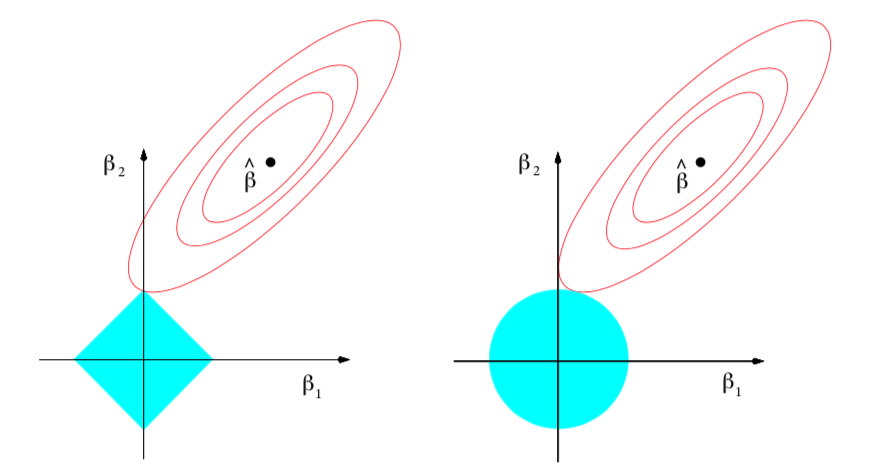
\includegraphics[scale=0.4]{img/ridge_lasso}
\caption{Constraints of ridge and lasso regression.}
\label{ridge_lasso}
\end{figure}

Also other penalization factors can be chosen, \ref{penalization}

\begin{figure}
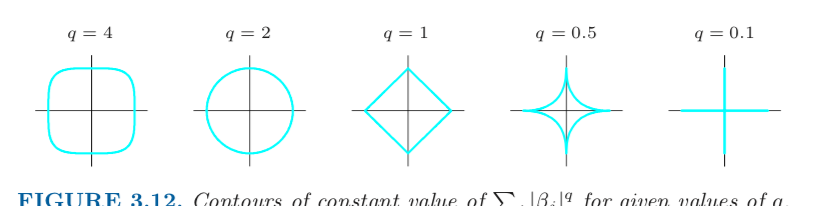
\includegraphics[scale=0.4]{img/penalization}
\caption{Shapes of different penalization factors.}
\label{penalization}
\end{figure}

\subsubsection{Least angle regression}
It is similar to forward stepwise. At first it identifies the variable most correlated with the response but instead of fitting it completely, it moves the variable toward its least squares value. As soon as another value gets correlated to the residual as the previous variable, the process is paused. The second variable joins the active set and their coefficients are moved together in a way that keeps their correlations tied and decreasing. The process is continued until all the variables are in the model.
\begin{algorithm}[!ht]
standardize the predictors to have $0$ mean and unit norm\;
$\mathcal{A}_k\leftarrow 0$\;
$r\leftarrow y-\bar{y}$, $\beta_i=0$ for $i\ne0$\;
\While {$|\mathcal{A}_k|<p$}{
find the predictor most correlated to $r$\;
insert the predictor in the active set $\mathcal{A}_k$\;

move the coefficients of the predictors in the active set to the direction defined by their joint least squares coefficient of the current residual, i.e.,
\begin{equation}
\delta_k = \left( X_{\mathcal{A}_k}^T X_{\mathcal{A}_k}\right)^{-1} X_{\mathcal{A}_k}^T r_k
\end{equation}
(where $\mathcal{A}_k$ is the current active set of variables) until some other competitor $x_l$ has as much correlation with the current residual\;
$r_k\leftarrow y - X_{\mathcal{A}_k}\beta_{\mathcal{A}_k}$
}
\end{algorithm}
After $min(N-1,p)$ steps we we arrive at the full least squares solution.
The coefficient profile evolves as
\begin{equation}
\beta_{\mathcal{A}_k} =  \beta_{\mathcal{A}_k} + \alpha \delta_k
\end{equation}

If to the LAR algorithm we add the following rule i.e.,

\textit{If a non-zero coefficient hits $0$, drop its variable from the active set of variables and recompute the current joint least squares direction.}

we get the same coefficient path of the lasso and this is called LAR(lasso). So this become an efficient solution to compute the Lasso problem, especially with $N>>p$ since Lasso can take more than $p$ steps while LAR require $p$ steps and it is efficient since it requires the same complexity as that of a single least squares fit using the $p$ predictors.

\subsection{Derived input directions methods}
When a large number of inputs is present, often there is a high correlation among them. In this case is convenient to regress on a new set inputs obtained form a linear combination of the original input.

\subsubsection{Principal component analysis}
First input must be standardized since this analysis depends on the scaling. The principal components are defined as  	
\begin{equation}
z_i = X v_i
\end{equation}
where $v_i$ are the column vectors of $V$ from the SVD decomposition of $X=UDV^T$ (recall that $z_m$ are orthogonal). The algorithm then regress $X$ on $z_1,\cdots, z_M$ for $M\le p$ and we have:

\begin{equation}
\hat{y}^{pcr}_{(M)} = \bar{y}\mathbf{1} + \sum_{m=1}^M \hat{\theta}_m z_m
\end{equation}
where $\hat{\theta}_m = \langle z_m, y\rangle/\langle z_m, z_m \rangle$. Since $z_m$ are linear combination of the original predictors $x_j$, we can express the solution as 

\begin{equation}
\hat{\beta}^{pcr}(M) = \sum_{m=1}^{M} \hat{\theta}_m v_m
\end{equation}
With $M=p$ we get the usual least squares. Principal component analysis discards the $p-M$ smallest eigenvalue components.

The value $M$ is suggested by cross-validation.
\subsubsection{Partial least squares}
This technique use a set of linear combinations of $y$ in addition to $X$ for the construction. It is not scale invariant so each $x_j$ must be standardized.
\begin{algorithm}
standardize $x_j$ to $0$ mean and $1$ variance\;
$\hat{y}^{(0)}\leftarrow \bar{y}\mathbf{1}$\;
$x_j^{(0)} \leftarrow x_j$ \;
\For{$m=1,\cdots, p$}
{
    $z_m  = \sum_{j=1}^p \hat{\phi}_{mj} x_j^{(m-1)}$ where $\hat{\phi}_{mj} = \langle x_j^{(m-1)}, y\rangle$ \; 
    $\hat{\theta}_m = \frac{\langle z_m, y\rangle}{\langle z_m, z_m\rangle} $\;
    $\hat{y}^m = \hat{y}^{(m-1)} + \hat{\theta}_m z_m$\;
    orthogonalize each $x_j^{m-1}$ w.r.t. $z_m: x_j^{(m)} = x_j^{(m-1)} - \frac{\langle z_m, x_j^{(m-1)}\rangle}{\langle z_m, z_m\rangle} z_m$, $j=1,\cdots, p$\;
}
Output the sequence of fitted vectors $\{\hat{y}^m\}_1^p$. Since ${z_l}_1^m$ are linear in $x_j$, so is $\hat{y}^{(m)} = X \hat{\beta}^{pls}(m)$. These coefficients can be recovered from the sequence of PLS transformations.
\end{algorithm}

Since PLS use $y$ to construct its directions, its solution path is not linear in $y$. It seeks direction with high variance and high correlation with the response while PCR only with high variance.

\subsection{Multioutput shrinkage and selection}
To apply selection and shrinkage methods in the multiple output case, one could apply a univariate technique individually to each outcome or si- multaneously to all outcomes, i.e., different $\lambda$ in Ridge or Lasso can be used for each output or the same value can be adopted.

\subsection{Other derived algorithms}
\subsubsection{Incremental forward stagewise}
\begin{algorithm}
$r\leftarrow y$ \;
$\beta_i =0$ for $i\ne 0$\;
find the (standardized) predictor $x_j$ most correlated with the residual \;
$\beta_j \leftarrow \beta_j + \delta_j$ where $\delta_j = \epsilon sign\left[\langle x_j, r \rangle\right]$ and $\epsilon >0$ small\;
$r\leftarrow r-\delta_j x_j$\;
Repeat the steps many times until the residuals are uncorrelated with the predictors.
\end{algorithm}

\subsubsection{The Dantzig selector}
$\cdots$

\subsubsection{The Grouped Lasso}
$\cdots$

\section{Bayesian inference}

\subsection{Introduction to Bayes' theorem}
Bayes' theorem is a formula that describes how to update the probabilities of hypotheses when given evidence. It follows simply from the axioms of conditional probability, but can be used to powerfully reason about a wide range of problems involving belief updates.

Given a hypothesis $H$ and evidence $E$, Bayes' theorem states that the relationship between the probability of the hypothesis $Pr(H)$, before getting the evidence, and the probability of the hypothesis after getting the evidence $Pr(H|E)$ is
\begin{equation}
Pr(H|E) = \frac{Pr(E|H)Pr(H)}{Pr(E)}
\end{equation}
Often there are competing hypothesis and the task is to determine which is the most probable.

This formula relates the probability of the hypothesis before getting the evidence $Pr(H)$, to the probability of the hypothesis after getting the evidence, $Pr(H|E)$: this term is generally what we want to know. For this reason, $Pr(H)$ is called the \textbf{prior probability}, while 
$Pr(H|E)$ is called the \textbf{posterior probability}. The factor that relates the two, $\frac{Pr(E|H)}{Pr(E)}$, is called the \textbf{likelihood ratio} and $Pr(E|H)$ is called \textbf{likelihood} which indicates the compatibility of the evidence with the given hypothesis.
$P(H|E)$ and $Pr(E|H)$ are called conditional probabilities. A conditional probability is an expression of how probable one event is given that some other event occurred (a fixed value) and Bayes' theorem centers on relating different conditional probabilities.

$Pr(E)$ is sometimes called \textbf{marginal likelihood} or model evidence this factor is the same for all the hypotheses being considered.

\subsection{Bayes inference}
Bayesian inference is a method of statistical inference in which Bayes' theorem is used to update the probability for a hypothesis as more evidence or information becomes available. Bayesian inference assumes the data were generated by a model with unknown parameters. From this, it tries to come up with beliefs about the likely  "true values" of the parameters of the model. The Bayesian approach differs from the standard (“frequentist”) method for inference in its use of a prior distribution to express the uncertainty present before seeing the data, and to allow the uncertainty remaining after seeing the data to be expressed in the form of a posterior distribution.

For this reason when writing down the Bayes theorem in these cases, formally also the conditional on the choice of the model should be written down:

\begin{equation}
Pr(\theta|\X,M) = \frac{Pr(\X|\theta,M)Pr(\theta|M)}{Pr(\X|M)}
\end{equation}
Here the hypothesis described in the previous paragraph is represented by a set of values for the parameters.

Once the model is stipulated, $Pr(X|\theta)$ can be evaluated for any given set of parameters: in this sense the likelihood is fixed once the model is fixed.
$Pr(\X|M)$ can be rexpressed as $Pr(\X|M) =\int Pr(\X|\theta,M)Pr(\theta|M)d\theta$. In this way it can be re-thought as a normalization factor of the sets of parameters since it is a summation over the all parameter space. However note that it \textbf{does depend} on the choice of the model. It can be seen also as asking the question \textit{how much is it probable to see the data we have seen given that the model $M$, without any claim about its parameters, generated those data}?

\subsection{Types of estimation}
It is the moment to clarify different types of estimation. We have already seen the Ordinary Least Square (OLS) estimation, and other types of estimation based on the definition of an error function.

We have also seen the \textbf{Maximum Likelihood Estimation (MLE)} approach, which maximizes the likelihood of the Bayes expression and how it is equivalent to OLS estimation in case of linear regression. (To be precise almost always the log-likelihood is maximized, first of all because of analytical convenience since many times we deal with exponentials coming from Gaussian distribution. Secondly for numerical precision: we are dealing with probabilities, numbers between $0$ and $1$ and since the range is quite small, underflow might be a problem.) The logarithmic instead extends the range by mapping numbers close to $0$ to $\infty$, resulting in a better precision.

The \textbf{Maximum A-Priori (MAP)} estimation maximizes the numerator of the Bayes expression, i.e., the likelihood times the prior, which means the likelihood is weighted by weights coming from the prior. When using a uniform distribution for the prior, MAP turns into MLE since we are assigning equal weights for each possible value. For example suppose we can assign six possible values to $\be$ and assume $P(\be_i)=1/6$:
\begin{equation}
\begin{aligned}
&\be_{MAP} = \argmax{\be}{\sum_i Pr(\x_i|\be) + \log P(\be)} =
\\&= \argmax{\be}{\sum_i Pr(\x_i|\be) +const}=\argmax{\be}{\sum_i Pr(\x_i|\be)} = \be_{MLE}
\end{aligned}
\end{equation}

When using a different prior, i.e., the simplification does not hold anymore.

\subsection{Conjugate distributions}
\label{conjugacy}
\begin{definition}{\textbf{Conjugate distributions}}
In Bayesian probability theory, if the posterior distribution $Pr(\theta|\X,M)$ is in the same probability space as the prior probability distribution $Pr(\theta|M)$, then the prior and posterior are called \textbf{conjugate distributions}, and the prior is called \textbf{conjugate prior for the likelihood function}. 
\end{definition}

As example consider the Gaussian distribution: \textbf{the Gaussian family is conjugate to itself (or self-conjugate) with respect to a Gaussian likelihood function}. If the likelihood is Gaussian, choosing Gaussian prior will ensure that also the posterior distribution is a Gaussian (see \ref{gaussian}). This means that the Gaussian distribution is a conjugate prior for the likelihood that is also Gaussian.

Consider the general problem of inferring a (continuous) distribution for a parameter $\theta$ given some datum or data $x$. From Bayes' theorem, the posterior distribution is equal to the product of the likelihood function $p(x|\theta, M)$ and the prior $p(\theta|M)$. Let the likelihood function be considered fixed; the likelihood function is usually well-determined from a statement of the data-generating process. It is clear that different choices of the prior distribution $p(\theta|M)$ may make the integral more or less difficult to calculate, and the product $p(x|\theta,M) \times p(\theta|M)$ may take one algebraic form or another. For certain choices of the prior, the posterior has the same algebraic form as the prior (generally with different parameter values). Such a choice is a conjugate prior. A conjugate prior is an algebraic convenience, giving a closed-form expression for the posterior; otherwise numerical integration may be necessary. Further, conjugate priors may give intuition, by more transparently showing how a likelihood function updates a prior distribution.
All members of the exponential family have conjugate priors.

In case of \textbf{classification} we are given a training set with input and output data. Once we have stipulated a model that could have generated output data, we want to find the best parameters of the model such that when those inputs are fed to the model we get those outputs. So the question becomes \textit{what is the best set of parameters $\theta$ for the model $M$ that could have generated the output $\y$ when the model has been fed with input data $\X$?}

In formula:
\begin{equation}
\label{ClassBayes}
Pr(\theta|\y,\X,M) = \frac{Pr(\y|\theta,\X,M)Pr(\theta|\X, M)}{Pr(\y|\X,M)}
\end{equation}

\subsubsection{Dataset likelihood}
\label{dataset likelihood}
\ref{dataset likelihood}
To be precise the likelihood is the likelihood of an entire dataset, since we are interested in all $\y$ and not in a single value $y$. $Pr(\y|\theta,\X,M)$ is then a joint density over all the responses in our dataset: $Pr(y_1, y_2, \cdots, y_n|\theta,\X,M)$. Evaluating this density at the observed points gives a single likelihood value for the whole dataset.	 Assuming that the noise at each data point is independent we can factorize as:
\begin{equation}
Pr(\y|\theta,\X,M) = \prod_{n=1}^N Pr(y_n|\x_n, \theta)
\end{equation}
We have not say that $y_n$'s are completely independent as otherwise it would not be worth trying to model the data at all. Rather, they are \textbf{conditionally independent} given a value $\theta$, i.e., the deterministic model.
Basically the model incorporates the dependency. Consider the following example, we have a set of data $(\y,\X)$ from which we want to predict the output $y_n$ given a new $\x_n$. Recalling from conditional probability that $P(A|B) = \frac{Pr(A\cap B)}{Pr(B)}$ we have:
\begin{equation}
P(y_n|\y,\x_n, \X) = \frac{Pr(y_n\cap \y|\x_n,\X)}{Pr(\y|\x_n,\X)}
\end{equation}
Note that actually $\y$ does not depend on $\x_n$: $Pr(\y|\x_n,\X) = Pr(\y|\X)$. Using independence:
\begin{equation}
P(y_n|\y,\x_n, \X) = \frac{Pr(y_n\cap \y|\x_n,\X)}{Pr(\y|\X)} = \frac{Pr(\y|\X) Pr(y_n|\x_n,\X)}{Pr(\y|\X)} = 
\end{equation}
[TO BE CONTINUED WAITING ON ANSWER ON CROSS-VALIDATED STACK EXCHANGE]

\section{Linear Classification}
For classification problem, in this section we assume the classification boundaries are linear, i.e., in the input hyperspace the points belonging to different classes can be separated by hyperplanes. 

\subsection{Linear regression of an Indicator matrix}
Suppose we have $K$ classes. For a single output we build a vector $\mathbf{y} = \left( y_1, \cdots, y_k\right)$ where $y_k=1$ if the class it belongs is the $k$ class. As output we will have the matrix $\mathbf{Y}$ of $0$ and $1$ with each row having a single $1$. We fit a linear regression model to each of the columns of $\mathbf{Y}$ simultaneously:
\begin{align*}
\hat{\mathbf{Y}} = \mathbf{X}\left( \mathbf{X}^T\mathbf{X}\right)^{-1}\mathbf{X}^T\mathbf{Y}
\end{align*}
We get a coefficient vector for each response column $y_k$, and hence a $(p+1) \times K$ matrix $\hat{\mathbf{B}} = \left( \mathbf{X}^T\mathbf{X}\right)^{-1}\mathbf{X}^T\mathbf{Y}$,where $\mathbf{X}$ will have $p+1$ columns with a leading column of 1 for the intercept.

Suppose we are given a new input $x$. Then the classification problem becomes:

\textit{compute the output $\hat{f}(x)^T = (1, x^T)\mathbf{\hat{B}}$ which is a $k$ vector
identify the largest component $\hat{G}(x) = \argmax{k \in \mathcal{G}} \hat{f}_k(x)$}.

With this approach we are basically estimating a conditional expectation, i.e., given the inputs $\x$ what is the probability the output is of class $k$? Mathematically $\E\left( y_k|X=x\right) =  Pr\left( G=k|X=x\right)$ since $y_k=1$.

Although the linear model guarantees $\sum_{k \in \mathcal{G}}\hat{f}_k=1$, as long as there is an intercept in the model, $\hat{f}_k(x)$ can be negative or bigger than one, especially when making predictions outside the hull of training data. Although this fact, this approach still works in many cases.

\textbf{An important limitation} is when $K\ge 3$. Even if the classes can still be separated by more than one linear boundaries, linear regression cannot find linear boundaries (because they are more than one?).

Quadratic regression might solve the problem, but a general rule is that if $k\ge3$ classes are lined up (their centroids are in the same line), a polynomial term with degree up to $k-1$ is  needed to solve the problem, and since the direction is arbitrary, cross-products terms might be needed too.

\subsection{Linear Discriminant analysis}
For optimal classification we have to know the class posteriors $Pr\left( G|X\right)$. Let $\pi_k$ be the prior probability of class $k$ with $\sum_k^K \pi_k=1$. Suppose $f_k(x)$ is the class conditional density.
From the Bayes theorem (?) we get 
\begin{equation}
Pr\left( G=k | X=x\right) = \frac{Pr\left( X=x |G=k \right)Pr(G=k)}{Pr(X=x)}
\end{equation}
% 
$Pr(G=k)$ is the prior probability $\pi_k$, $Pr\left( X=x |G=k \right)$ is the class conditional density while the denominator can be rewritten using the \textbf{Total Probability Theorem} as
\begin{align}
&Pr(X=x) = \sum_{l=1}^{K} Pr(X=x|G=l) Pr(G=l) = \sum_{l=1}^{K} Pr(X=x|G=l) \pi_l\\
&\Rightarrow Pr\left( G=k | X=x\right) =\frac{f_k(x)\pi_k}{\sum_{l=1}^Kf_l(x)\pi_l}
\end{align}

The goodness of classification mostly rely on $f_k(x)$ and many techniques use models for class densities:
\begin{itemize}
\item linear and quadratic discriminant analysis use Gaussian densities;
\item mixtures of Gaussians allow for non-linear boundaries;
\item Naive Bayes models assume that each class density is a product of marginal densities i.e., inputs are conditionally independent in each class.
\end{itemize}
Modelling each class density as a multivariate Gaussian we have
\begin{equation}
f_k(x) = \frac{1}{(2\pi)^{\frac{p}{2}}|\sum_k|^{\frac{1}{2	}}} e^{-\frac{1}{2}\left( x-\mu_k\right)^T\Sigma_k^{-1}\left( x-\mu_k\right)}
\end{equation}

\textbf{Linear Discriminant analysis assumes equal covariance matrices for all classes}. Taking as comparison between two classes the log-ratio, we have
\begin{equation}
\begin{aligned}
\log &\frac{Pr(G=k|X=x)}{Pr(G=l|X=x)} = \log \frac{f_k(x) \pi_k}{f_l(x) \pi_l} = \log \frac{ \pi_k}{ \pi_l} + \log\frac{f_k(x)}{f_l(x) } =\\
&= \log \frac{ \pi_k}{ \pi_l} + \log\frac{e^{-\frac{1}{2}\left( x-\mu_k\right)^T\Sigma^{-1}\left( x-\mu_k\right)}}{e^{-\frac{1}{2}\left( x-\mu_l\right)^T\Sigma^{-1}\left( x-\mu_l\right)} }   =  \\
&=log \frac{ \pi_k}{ \pi_l} - \frac{1}{2}\left( x-\mu_k\right)^T\Sigma^{-1}\left( x-\mu_k\right) - \left( -\frac{1}{2}\right)\left( x-\mu_l\right)^T\Sigma^{-1}\left( x-\mu_l\right) =\\
&= log \frac{ \pi_k}{ \pi_l} - \frac{1}{2}\left[\left( x-\mu_k\right)^T\Sigma^{-1}\left( x-\mu_k\right) + \left( x-\mu_l\right)^T\Sigma^{-1}\left( \mu_l - x\right)\right] =\\
&= log \frac{ \pi_k}{ \pi_l} - \frac{1}{2}\left[\left( 2x-\mu_k-\mu_l\right)^T\Sigma^{-1}\left( \mu_l-\mu_k\right) \right] =\\
&= log \frac{ \pi_k}{ \pi_l} +\frac{1}{2}x^T\Sigma^{-1}\left( \mu_k-\mu_l\right)- \frac{1}{2}\left( \mu_k+\mu_l\right)^T\Sigma^{-1}\left( \mu_k-\mu_l\right) =\\
\end{aligned}
\end{equation}
which is linear in $x$, so all decision boundaries are linear (i.e., they are hyperplanes in $p$ dimensions). If the common covariance matrix is spherical, i.e., $\Sigma=\sigma^2 I$ and the class priors are equal, each boundary that separates two classes is the perpendicular bisector of the segment joining the centroids of the two classes.

The linear discriminant functions of each class are 
\begin{equation}
\delta_k(x)  = x^T \Sigma^{-1}\mu_k -\frac{1}{2}\mu_k^T+log\pi_k
\end{equation}
We do not know the parameters of the Gaussian distribution and we must estimate them from the training data:
\begin{align}
&\hat{\pi}_k = \frac{N_k}{N}\\
&\hat{\mu}_k = \sum_{g_i=k}\frac{x_i}{N_k}\\
&\hat{\Sigma} = \sum_{k=1}^K\frac{(x_i-\hat{\mu}_k)(x_i-\hat{\mu}_k)^T}{(N-K)}
\end{align}

\textbf{Note} that LDA does not use Gaussian assumption for the features.

\subsubsection{Decision rule}
Consider two classes $1$ and $2$. LDA classifies to class $1$ if
\begin{equation}
x^T\hsi \hmu_1 - \frac{1}{2}\hmu_1^T\hsi\hmu_1 + \log \hpi_1 >x^T\hsi \hmu_2 - \frac{1}{2}\hmu_2^T\hsi\hmu_2 + \log \hpi_2
\end{equation}
to class $2$ if $<$ holds. In such case there is a correspondence between LDA and linear regression classification if the two classes are coded with $+1$ and $-1$. In this case the coefficient vector from least squares is proportional to the LDA direction. However unless $N_1=N_2$, the intercepts are different and so are the decision rules.

With more than $2$ classes, linear regression is not able to classify correctly while LDA does.

\subsection{Quadratic Discriminant analysis}
If we do not assume equal covariance, the squared term in $x$ does not cancel out and we get quadratic discriminant functions:
\begin{equation}
\label{QDA}
\begin{aligned}
\delta_k  (x) &= -\frac{1}{2} \log |\Sigma_k| -\frac{1}{2} \left( x - \mu_k \right)^T \si_k\left( x - \mu_k \right) + \log \pi_k
\end{aligned}
\end{equation}
The decision boundaries between two classes are quadratic functions.

\textbf{Note}: QDA does not differ much from LDA applied the enlarged quadratic polynomial input space but generally QDA is preferred in this case.

The estimates are similar but the covariance matrix must be estimated for each class. When $p$ is large, this means a dramatic increase in the number of parameters, considering we only need the differences $\delta_k (x) - \delta_l(x)$. LDA needs $(K-1)\times (p+1)$ parameters, while QDA needs $(K-1) \times \left(p\left(p+3\right)/2 +1\right)$.

\subsection{Regularized discriminant analysis}
This method shrinks the separate covariances of QDA towards a common covariance as in LDA. In a way it is similar to ridge regression. The regularized covariance matrices have the form:

\begin{equation}
\hS_k(\alpha) = \alpha\hS_k+(1-\alpha) \hS
\end{equation}
with $\alpha \in [0,1]$, the two extremes being LDA and QDA. $\alpha$ can be chosen on the validation data or by cross-validation.

Similarly we can allow $\hS$ to be shrunk toward the scalar covariance:
\begin{equation}
\hS(\gamma) = \gamma\hS+(1-\gamma) \hat{\sigma}^2 I
\end{equation}
with $\gamma \in [0,1]$
so we get a more general family of covariances
\begin{equation}
\hS_k(\alpha, \gamma) = \alpha\hS_k+\left(1-\alpha\right) \left(\gamma\hS+\left(1-\gamma\right) \hat{\sigma}^2 I\right)
\end{equation}

\subsection{Computation}
Computation of LDA and QDA is simplified by diagonalizing the covariance matrices with the singular value decomposition $\hS_k = U_kD_kU_k^T$. The terms in \ref{QDA} become
\begin{align}
&\begin{aligned}
&\left( x - \mu_k \right)^T \si_k\left( x - \mu_k \right)= \left( x - \mu_k \right)^T \left(U_kD_kU_k^T\right)^{-1}\left( x - \mu_k \right) =\\
&= \left( x - \mu_k \right)^T U_kD_k^{-1}U_k^T\left( x - \mu_k \right) =  \left[ U_k^T\left( x - \mu_k \right)\right]^T D_k^{-1}\left[ U_k^T\left( x - \mu_k \right)\right]
\end{aligned}\\
& \log |\hS_k| = \sum_l \log d_{kl}
\end{align}
Considering the above steps, LDA classifier can be seen as performing the following steps:
\begin{itemize}
\item sphere the data w.r.t. the common covariance estimate: $X*\leftarrow D^{-\frac{1}{2}} U^T X$. The common covariance estimate fof $X*$ will now be the identity.
\item Classify to the closest centroid in the transformed space, modulo the effect of the class prior probability $\pi_k$(?)
\end{itemize}
\subsection{Regularized-rank linear discriminant analysis}
Consider $K=2$ with two centroids and the input is $2$, i.e., input points are on a plane. Given an input point, for classification purposes what matters is not the distance in the $p$ space of such point from the two centroids but rather the distance from the two centroids of the projection of this point on the line joining them (\ref{proj}). So basically instead of using the $2$ dimensions, we are calculating the distance in one dimension, a line. If $K=3$ then the points are projected onto a plane (2d), of course in this case it is convenient if $p>2$.

More generally the $K$ centroids in $p$-dimensional input, lie in an affine subspace of dimensions $\le K-1$ and if $p>$ is much larger than $K$ this will be a considerable drop in dimension.


\begin{figure}
\centering
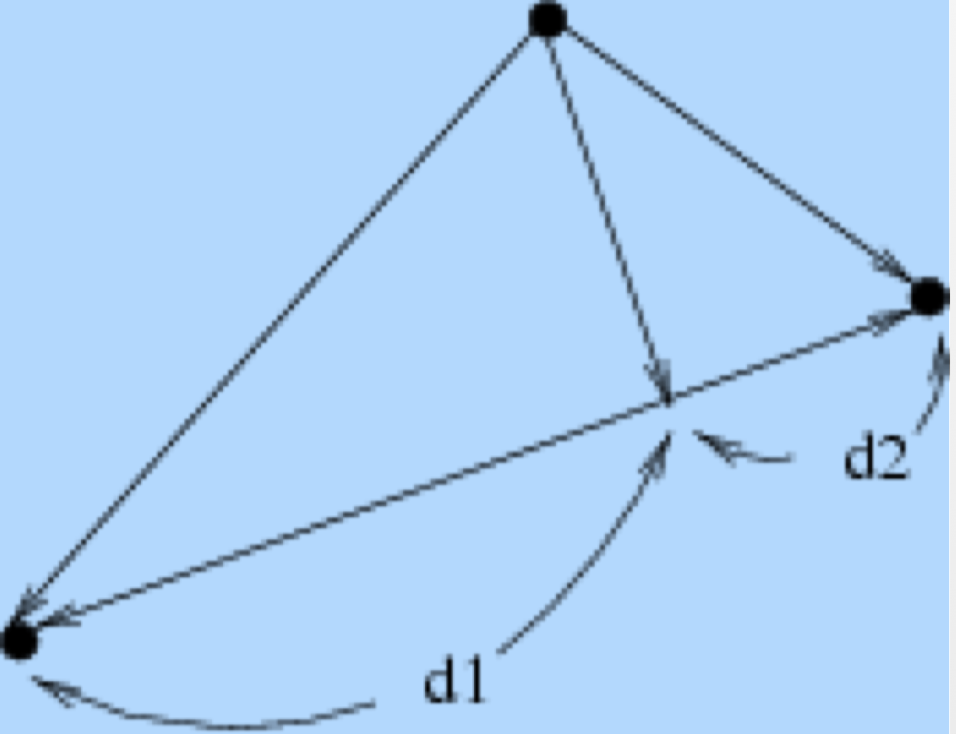
\includegraphics[scale=0.4]{img/proj}
\caption{...}
\label{proj}
\end{figure}

If $K>3$ we can look for a $L<K-1$ dimensional subspace optimal for LDA. Fisher defined \textit{optimal} such that the projected centroids were spread out as much as possible in terms of variance.
This problem, finding the principal component subspaces of the centroids, involves the following steps:
\begin{itemize}
\item compute the $k\times p$ matrix of class centroids $M$ and the common covariance matrix $W$ for within-class covariance;
\item compute $M*=MW^{-\frac{1}{2}}$ using the eigen-value decomposition;
\item compute $B*$, the covariance matrix of $M*$ ($B$ for between class covariance) and its eigenvalue decomposition $B^{*}=V^{*}D_BV^{*T}$. The columns $v^*_l$ from the first to the last define the coordinates of optimal subspaces.
\end{itemize}
The $lth$ discriminant variable is given by $Z_l =  v_l^TX$ with $v_l=W^{-\frac{1}{2}} v^*_l$.  Although the direction joining the centroids separates the means as much as possible(maximizes the between class covariance), there is an overlap between the projected classes due to the nature of covariances. Taking the covariances into account reduce the overlap and that is what we are doing (\ref{cov}).

\begin{figure}
\centering
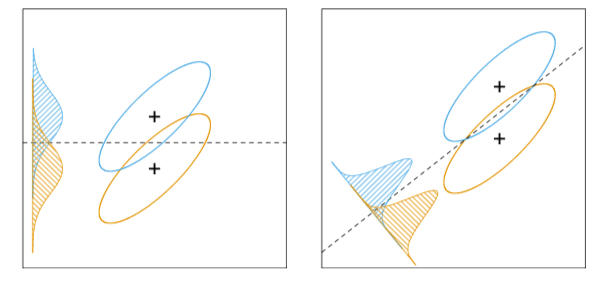
\includegraphics[scale=0.4]{img/cov}
\caption{Covariance.}
\label{cov}
\end{figure}

The between-class variance $Z$ is $a^TBa$ and the within class variance is $a^TWa$, with $B+W=T$, the total covariance matrix of $X$.
Fisher's problem maximizes the \textit{Rayleigh quotient}:

\begin{equation}
max_{a} \frac{a^TBa}{a^TWa}
\end{equation}

This is a generalized eigenvalue problem, with $a$ given by the largest eigenvalue. Similarly one can find the next direction $a_2$, orthogonal in $W$ to $a_1$, such that $a^T_2 Ba_2/a^T_2 Wa_2$ is maximized; the solution is a$_2 = v_2$, and so on. $a_l$ are the \textit{discriminant coordinates} or \textit{canonical variates}, different from discriminant functions.

The reduced subspaces can be used both for visualization and classification by limiting the distance between centroids to the chosen subspace. However, when doing this, due to the Gaussian classification, a correction factor of $\log \pi_k$ is needed. The misclassification is given by the overlapping area in \ref{cov} between the two densities. When both classes have the same priors $\pi_k$ as in the figure, the optimal cut-point is the midway between projected means, if not the cut-point is moved towards the smaller class to have a better error rate.

For $2$ classes one can derive the linear rule using LDA, and then choosing the cut-point to minimize misclassification error.

\subsection{Logistic regression}
The idea behind logistic regression is to still exploit a linear model $x^T\beta$ but having its output representing a probability, i.e., constrained between $0$ and $1$. This part is performed using the sigmoid function

\begin{equation}
p=\sigma(q) = \frac{1}{1+e^{-q}}
\end{equation}
Inverting the terms we get 
\begin{equation}
\label{logit}
q = -\log\frac{1-p}{p} = \log \frac{p}{1-p} 
\end{equation}
\ref{logit} is called \textbf{logit function}. As $q$ increases to $\infty$, the output of the sigmoid gets closer to $1$; instead when it diverges to $-\infty$ we get $0$. Suppose we have just 2 classes or equivalently a binary classifier that tells the probability of an event to happen: $Y_n=1$ when the event happens and $Y_n=0$ when it does not. We can express the probabilities output by our classifier when new input data $x_{new}$ are observed as:
\begin{equation}
\begin{aligned}
&P(G=1|x_n, \beta) =  \frac{1}{1+e^{-\beta^T\x_{new}}}\\
&P(G=0|x_n, \beta) = 1- \frac{1}{1+e^{-\beta^T\x_{new}}} = \frac{e^{-\beta^T\x_{new}}}{1+e^{-\beta^T\x_{new}}}
\end{aligned}
\end{equation}

These equations can be combined in a single equation:
\begin{equation}
P(G=g|x_n, \beta) =  P(G=1|x_n, \beta)^{g} P(G=0|x_n, \beta)^{g-1}
\end{equation}

Taking the log-ratio between the two probabilities we have:
\begin{equation}
\begin{aligned}
\log \frac{P(Y_n=0|x_n, \beta)}{P(Y_n=1|x_n, \beta)} =  \log \frac{\frac{e^{-\beta^T\x_{new}}}{\cancel{1+e^{-\beta^T\x_{new}}}}}{\frac{1}{\cancel{1+e^{-\beta^T\x_{new}}}}} = -\beta^T\x_{new}
\end{aligned}
\end{equation}
So we are using lines (or hyperplanes) to separate the two classes.

\subsubsection{Multinomial logistic regression: more than 2 classes}
Now suppose we have more than two classes and we still want to separate those classes with linear functions, which means we will have a hyperplane separating two classes. We have $K$ possible outcomes. We can think to run $K-1$ independent binary logistic regressions with one class chosen as \textbf{pivot}, generally the one corresponding to class $K$, and with the other $K-1$ classes separately regressed against the pivot:
%LR models the posterior probabilities of the classes as linear function in $x$, while ensuring they sum up to $1$.
%The model has the form
\begin{equation}
\begin{aligned}
&\log \frac{Pr\left(G=1|X=x\right)}{Pr\left(G=K|X=x\right)} = \beta_1^T x \\
&\log \frac{Pr\left(G=2|X=x\right)}{Pr\left(G=K|X=x\right)} = \beta_2^T x\\
\vdots\\
&\log \frac{Pr\left(G=K-1|X=x\right)}{Pr\left(G=K|X=x\right)} = \beta_{\left(K-1\right)}^T x
\end{aligned}
\end{equation}
The choice of the pivot class used as denominator is arbitrarily and the estimates are equivalent under different choices.

Summing the probability of each class we must get $1$:
\begin{equation}
\begin{aligned}
&\sum_{l=1}^{K} Pr\left(G=l|X=x\right) = 1 \Rightarrow Pr\left(G=K|X=x\right)+ \sum_{l=1}^{K-1} Pr\left(G=l|X=x\right)=1\\
&\Rightarrow Pr\left(G=K|X=x\right) +\sum_{l=1}^{K-1} Pr\left(G=K|X=x\right)e^{\beta_l^Tx}=1\\
&\Rightarrow Pr\left(G=K|X=x\right)= \frac{1}{1+\sum_{l=1}^{K-1} e^{\beta_l^Tx}}
\end{aligned}
\end{equation}

So we can re-express the probabilities as:

\begin{equation}
Pr\left(G=k|X=x\right) = \frac{e^{\beta_{k}^T x}}{1+\sum_{l=1}^{K-1} e^{\beta_l^Tx}}
\end{equation}

\paragraph{\textbf{Softmax function}} We do not have anymore the sigmoid function, instead we have used another function named \textbf{softmax} that as the sigmoid takes any real value as input and outputs a value between $0$ and $1$. The difference mostly relies on the denominator used for normalization factor since the sigmoid is a 2D curve while the softmax can have higher dimensionality (for 2D it corresponds to the sigmoid).

\subsubsection{Fitting logistic regression}
From now on we will consider a logistic regression for just two classes. 

As seen in \ref{ClassBayes}, we want to find the best parameters for the chosen model according to some criteria. First let us apply the Bayes theorem:
\begin{equation}
Pr\left(\be|\y,\X,M\right) = \frac{Pr\left(\y|\be,\X,M\right) Pr(\be,M)}{Pr(\y|\X,M)}
\end{equation}
\textbf{From now on we will not write the conditional on the model for seek of brevity but we know it exists}.

This formula tells we want to find the coefficients given some input and output data. Let us analyse each term:
\begin{itemize}
\item $Pr(\be)$ (\textbf{prior distribution}): this is the prior belief about the parameters without seeing the data. As prior, we will use a Gaussian distribution with $0$ mean:  $\CMcal{N}(0, \sigma^2\I)$. In this way the parameters will depend on $\sigma^2$: more formally we should write $Pr(\be|\sigma)$ but we will skip. Although the choice of the Gaussian distribution with $0$ mean is analytically convenient as seen in \ref{conjugacy}, we will not rely on conjugacy.
\item $Pr\left(\y|\be,\X\right)$ (\textbf{likelihood}): we will assume $y$ are conditionally independent (\ref{dataset likelihood}):
\begin{equation}
Pr(\y|\X, \be) = \prod_{n=1}^N Pr(y_n|\x_n, \be)
\end{equation}
Since in this case we have a binary variable, instead of a Gaussian random variable, suitable for real values distribution, we will consider a binary random variable $Y_n$ characterised by the probability of the second class:
\begin{equation}
Pr(\y|\X, \be) = \prod_{n=1}^N Pr(Y_n=y_n|\x_n, \be)
\end{equation}
\item $Pr(\y|\X)$(\textbf{marginal likelihood}): It can be expressed as 
\begin{equation}
Pr(\y|\X) = \int Pr\left(\y|\be,\X\right) Pr(\be) d\be
\end{equation}
\end{itemize}

So the numerator can be calculated and results in a Gaussian function not in standard form (\ref{gaussian}). The denominator, or marginal likelihood, as we have seen can be expressed as $Pr(\y|\X) = \int Pr\left(\y|\be,\X\right) Pr(\be) d\be$. Mathematically this integral has no close solution since (again see \ref{gaussian}) and the impossibility of the integral of $e^{-x^2})$, unless an ad-hoc prior distribution is chosen.

When we cannot directly compute the posterior density (due to the denominator), we have three options:
\begin{enumerate}
\item find the single value $\be$ that correspond to the highest value of the posterior. This is equivalent to find the value $\be$ that maximize the numerator since the denominator is not a function of $\be$ but a numerical value.
\item Approximate $Pr(\be|\X, \y)$ with some other density that we can compute analytically.
\item Sample directly from the posterior $Pr(\be|\X,\y)$ knowing only the numerator.
\end{enumerate}

The first method is simple and hence popular but it is not very "Bayesian", since we will make predictions of new data based on a single value and not a distribution. The whole Bayesian theory is based on making an hypothesis and getting feedback from the data that can validate or not that hypothesis. Also when using a distribution we get also measures on how confident we are about the estimated model. For example when estimating a Gaussian distribution, we estimate the coefficients $\mu$ and $\sigma^2$: the smallest the latter value the more confident we are about the model. When using a single value we loose this piece of information.

With the second method we get a density easy to work with but if the chosen density is very different from the posterior our model will not be very reliable.

The third method samples from the posterior and hence to get a good approximation but it can be difficult.

\subsubsection{First method: point estimation, the MAP solution}
We have seen that in some cases we cannot compute the posterior but we can compute the numerator of the expression, i.e., the prior multiplied by the likelihood. The value that maximizes the posterior is also the value that maximizes the numerator. We have already seen a likelihood maximization procedure in \ref{likelihoodMax}; here we are maximizing the likelihood times the prior. This solution is the \textbf{maximum a posteriori (MAP)} estimate.

\paragraph{The Newton-Raphson method}
The Newton-Raphson method finds the points where $f(x)=0$. Starting from an estimation $x_n$ of such points, the estimation is updated by moving to the point where the tangent to the function at $x_n$ passes throw the x-axis. This point is computed by approximating the gradient as a change in $f(x)$ divided by a change in $x$:

\begin{figure}
\centering
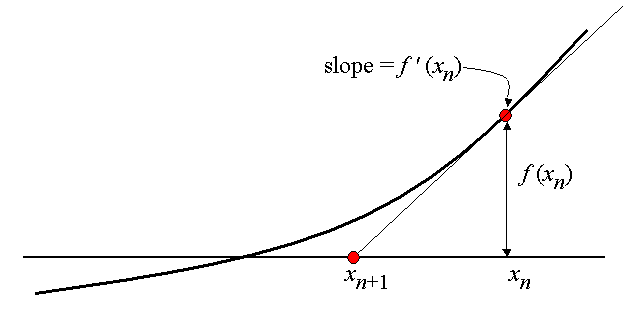
\includegraphics[scale=0.3]{img/NewtonRaphson}
\caption{Newton-Raphsone example.}
\end{figure}

\begin{equation}
\begin{aligned}
f'(x_n) = -\frac{f(x_n)-0}{x_n -x_{n+1}}\\
\Rightarrow x_{n+1} = x_n -\frac{f(x_n)}{f'(x_n)}
\end{aligned}
\end{equation}
Instead of finding the point for which $f(x)=0$, we want to find the point where its derivative is $0$. Hence we substitute $f(x)$ with $f'(x)$ and $f'(x)$ with $f''(x)$. In this way the method can be used to find points where the gradient passes through $0$, i.e., minima, maxima and points of inflections:
\begin{equation}
\begin{aligned}
f''(x_n) = -\frac{f'(x_n)-0}{x_n -x_{n+1}}\\
\Rightarrow x_{n+1} = x_n -\frac{f'(x_n)}{f''(x_n)}
\end{aligned}
\end{equation}
When dealing with vectors, $f'(x)$ is replaced by the vector of partial derivatives evaluated at $x_n$ and $\frac{1}{f''(x_n)}$ is replaced by the inverse of the Hessian matrix $\frac{-\partial^2 f(x)}{\partial \x \partial \x^T}$.

\paragraph{Derivation}
As already done, instead of maximizing the function itself, we maximize its logarithmic. Apart from the mathematical convenience this is also the advantage of avoiding underflow: we are dealing with probabilities, number between $0$ and $1$ and these might be too small to have a sufficient numerical precision. The logarithmic, as the numbers go to $0$, makes the number goes to infinity, guaranteeing a better numerical precision.
 Since we cannot compute the derivative and set it to $0$, we use the Newton-Raphson procedure. Let us call the numerator $g(\be,\X,\y) = Pr(\y|\be,\X)Pr(\be|\X)$:

\begin{equation}
\be' = \be - \br{\frac{\partial^2\log g(\be,\X,\y)}{\partial \be \partial \be^T}}^{-1} \frac{\partial \log g(\be,\X,\y)}{\partial \be}
\end{equation}

The procedure is iterative and stops when the gradient is $0$. To check the point we have converged to corresponds to a minimum we check the Hessian matrix is negative definite.

Before computing the derivatives we re-express $g(\be,\X,\y)$.

\begin{equation}
\begin{aligned}
&\log g(\be,\X,\y) = \sum_{n=1}^N \log Pr(Y_n=y_n|\x_n, \be) + \log Pr(\be|\sigma^2) = \\
&=  \sum_{n=1}^N \log \left[\br{\frac{1}{1+e^{-\be^T\x_n}}}^{y_n} \br{\frac{e^{-\be^T\x_n}}{1+e^{-\be^T\x_n}}}^{1-y_n}\right] + \log Pr(\be|\sigma^2) =
\end{aligned}
\end{equation}
We denote $P_n=P(Y_n=1|\be, \x_n) = \frac{1}{1+e^{-\be^T\x_n}}$:
\begin{equation}
\begin{aligned}
&\log g(\be,\X,\y) =  \sum_{n=1}^N \log P_n^{y_n} +\log(1-P_n)^{1-y_n}+ \log Pr(\be|\sigma^2) =
\end{aligned}
\end{equation}
Racalling
\begin{equation}
\begin{aligned}
Pr(\be|\sigma^2)  =& \frac{1}{\sqrt{(2\pi)^D|\Sigma|}} e^{-\frac{\br{\be-\cancel{\mu}}^T\br{\be-\cancel{\mu}}}{2\sigma2}}\\
\Rightarrow\log g(\be,\X,\y) =&  \sum_{n=1}^N \log P_n^{y_n} +\log(1-P_n)^{1-y_n} -\frac{D}{2}\log(2\pi) - D\log\sigma +\\
&- \frac{1}{2\sigma^2} \be^T\be
\end{aligned}
\end{equation}

Now we can take the derivative:
\begin{equation}
\label{devg}
\begin{aligned}
&\frac{\partial \log g(\be,\X,\y)}{\partial \be} = - \frac{1}{\sigma^2} \be + \sum_{n=1}^N \frac{y_n}{P_n}\frac{\partial P_n}{\partial \be} + \frac{1-y_n}{1-P_n}\frac{\partial (1-P_n)}{\partial \be} =\\
&=\frac{\partial \log g(\be,\X,\y)}{\partial \be} = - \frac{1}{\sigma^2} \be + \sum_{n=1}^N \frac{y_n}{P_n}\frac{\partial P_n}{\partial \be} - \frac{1-y_n}{1-P_n}\frac{\partial P_n}{\partial \be}
\end{aligned}
\end{equation}

Now we must calculate $\frac{\partial P_n}{\partial \be}$:
\begin{equation}
\label{devPn}
\begin{aligned}
\frac{\partial P_n}{\partial \be} =& \frac{\partial}{\partial \be} \frac{1}{1+e^{-\be^T\x_n}} = \frac{\partial}{\partial \be} \br{1+e^{-\be^T\x_n}}^{-1} =\\
=& \frac{1}{\br{1+e^{-\be^T\x_n}}^2}  \frac{\partial}{\partial \be} \br{1+e^{-\be^T\x_n}} = \\
=&  -\x_n \frac{e^{-\be^T\x_n}}{\br{1+e^{-\be^T\x_n}}^2}   = -x_n \frac{1}{\br{1+e^{-\be^T\x_n}}}\frac{e^{-\be^T\x_n}}{\br{1+e^{-\be^T\x_n}}} =\\
=& -\x_nP_n \br{1-P_n}
\end{aligned}
\end{equation}
Substituting in \ref{devg}:
\begin{equation}
\begin{aligned}
\frac{\partial \log g(\be,\X,\y)}{\partial \be} =&  - \frac{1}{\sigma^2} \be + \sum_{n=1}^N \frac{y_n}{P_n}\frac{\partial P_n}{\partial \be} - \frac{1-y_n}{1-P_n}\frac{\partial P_n}{\partial \be} =\\
=&- \frac{1}{\sigma^2} \be + \sum_{n=1}^N \frac{y_n}{P_n}\left[-\x_nP_n \br{1-P_n}\right]+ \\
&\quad  - \frac{1-y_n}{1-P_n}\left[-\x_nP_n \br{1-P_n}\right] =\\
=& - \frac{1}{\sigma^2} \be + \sum_{n=1}^N -y_n\x_n \br{1-P_n} - (1-y_n)(-\x_nP_n ) = \\
=& - \frac{1}{\sigma^2} \be + \sum_{n=1}^N \x_n (y_n-P_n)
\end{aligned}
\end{equation}

Now we must compute the Hessian matrix:
\begin{equation}
\begin{aligned}
&\frac{\partial^2 \log g(\be,\X,\y)}{\partial \be \partial\be^T}  = \frac{\partial}{\partial \be^T} \br{- \frac{1}{\sigma^2} \be + \sum_{n=1}^N \x_n (y_n-P_n)} =
\\ &=- \frac{1}{\sigma^2} \I -\sum_{n=1}^N \x_n \frac{\partial P_n}{\partial \be^T} = - \frac{1}{\sigma^2} \I - \sum_{n=1}^N \x_n \x_n^TP_n \br{1-P_n}
\end{aligned}
\end{equation}
where we used the result from \ref{devPn}.

Note that the 2 terms are negative definite, hence the Hessian is always negative definite. Therefore there can only be one optimum and it must be the minimum.

The decision boundary is the one for which $Pr(Y_n=1|\x,\hat{\be}=0.5)$.

The steps above can be done for any prior and likelihood combination. In some cases the posterior might have several maxima and or some minima and it become difficult to know if the maximum is a global optimum.


The \textit{Elements of Statistical Learning} book instead of maximizing posterior (or equivalently the numerator), it maximizes the likelihood.
Let us express $Pr\left(G=k|X=x\right)=p_k(x,\theta)$ with $\theta = \left\lbrace \beta_{10},\beta_1^T,\cdots, \beta_{\left(K-1\right)0},\beta_{K-1}^T\right\rbrace$
and let us define the log-likelihood
\begin{equation}
\ell(\theta) = \sum_{i=1}^N \log p_{g_i}\left(x_i, \theta\right)
\end{equation}

Consider just two classes with responses $0$, $1$ and let $p_1(x,\theta) =p(x,\theta) $ and $p_2(x,\theta) =1-p(x,\theta)$. Recall that having two classes $\sum_{l=1}^{K-1} e^{\beta_{l0}+\beta_l^Tx_i} = e^{\beta_{10}+\beta_1^Tx_i}$. The log-likelihood can be written as:
\begin{equation}
\begin{aligned}
&\ell(\beta) = \sum_{i=1}^N \left\lbrace y_i \log p\left(x_i,\beta\right) + \left(1-y_i\right) \log \left(1-p\left(x_i,\beta\right)\right)\right\rbrace =\\
&=\sum_{i=1}^N y_i \log \frac{e^{\beta_{10} +\beta_{1}^T x_i}}{1+\sum_{l=1}^{K-1} e^{\beta_{l0}+\beta_l^Tx_i}}  +\\
& \quad\quad + \sum_{i=1}^N \left(1-y_i\right) \log \left(1-\frac{e^{\beta_{10} +\beta_{1}^T x_i}}{1+\sum_{l=1}^{K-1} e^{\beta_{l0}+\beta_l^Tx_i}}\right)= \\
&= \sum_{i=1}^N  y_i \log \frac{e^{\beta_{10} +\beta_{1}^T x_i}}{1+e^{\beta_{10}+\beta_1^Tx_i}} + \\
&\quad\quad +\sum_{i=1}^N  \left(1-y_i\right) \log \left(1-\frac{e^{\beta_{10} +\beta_{1}^T x_i}}{1+e^{\beta_{10}+\beta_1^Tx_i}}\right) = \\
&=\sum_{i=1}^N y_i \left(\log e^{\beta_{10} +\beta_{1}^T x_i} -\log \left(1+ e^{\beta_{10}+\beta_1^Tx_i}\right) \right) + \\
& \quad\quad + \sum_{i=1}^N  \left(1-y_i\right) \log \frac{1}{1+ e^{\beta_{10}+\beta_1^Tx_i}} = \\
&=\sum_{i=1}^N y_i \left(\log e^{\beta_{10} +\beta_{1}^T x_i} -\log \left(1+ e^{\beta_{10}+\beta_1^Tx_i}\right) \right) + \\
& \quad\quad - \sum_{i=1}^N\left(1-y_i\right) \log \left(1+ e^{\beta_{10}+\beta_1^Tx_i}\right) = \\
&=\sum_{i=1}^N \left\lbrace y_i \left(\beta_{10} +\beta_{1}^T x_i \right) -log \left(1+ e^{\beta_{10}+\beta_1^Tx_i}\right) \right\rbrace
\end{aligned}
\end{equation}
Here $\beta = \left[ \beta_{10}, \beta_1\right]$. To maximize the log-likelihood we set the derivative to $0$:
\begin{equation}
\frac{\partial \ell(\beta)}{\partial \beta} = \sum_{i=1}^N x_i  (y_i - p(x_i, \beta) = 0
\end{equation}

Using the \textit{Newton-Raphson} algorithm that requires the second-derivative:
\begin{align}
&\frac{\partial^2 \ell(\beta)}{\partial \beta \partial \beta^T} = -\sum_{i=1}^N x_ix_i^T   p(x_i, \beta) (1-p(x_i, \beta)\\
&\Rightarrow \beta^{new} = \beta^{old} - \left( \frac{\partial^2 \ell\left( \beta\right) }{\partial \beta \partial \beta^T} \right)^{-1}\frac{\partial \ell(\beta)}{\partial \beta}
\end{align}
Using the matrix notation,
\begin{align}
\frac{\partial \ell(\beta)}{\partial \beta} =  X^T (y-p) \\
\frac{\partial^2 \ell(\beta)}{\partial \beta \partial \beta^T} = -X^TWX
\end{align}
So the Newton step becomes

\begin{equation}
\begin{aligned}
&\beta^{new} = \beta^{old} +(X^TWX)^{-1}X^T(y-p) = \\
&=(X^TWX)^{-1}X^TW\left(X\beta^{old}+W^{-1} \left(y-p\right)\right) =\\
&= \left(X^TWX\right)^{-1} X^TWz
\end{aligned}
\end{equation}
with
\begin{equation}
z = X\beta^{old}+ W^{-1} (y-p)
\end{equation}
sometimes known as the adjusted response. This algorithm is known as \textbf{iteratively reweighted least squares (IRLS)} since each iteration solves the weighted least square problem:
\begin{equation}
\beta^{new} \leftarrow \argmin{\beta}{\left(z-X\beta\right)^TW\left(z-X\beta\right)}
\end{equation}
$\beta=0$ seems a good starting value. Convergence is never guaranteed but typically the algorithm does converge, since the log-likelihood is concave but overshooting can occur. In the rare cases that the log-likelihood decreases, step size halving will guarantee convergence.

For $K>2$ we still use the iteration procedure but we will have a $K-1$ vector response and a non-diagonal weight matrix per observation. In this case it is better to work with the vector $\theta$ directly.

\subsubsection{Second method: Laplace approximation}
There are many approximation methods but the most common is the Laplace approximation. The idea is to approximate the density of interest with a Gaussian.

Choosing a Gaussian means choosing a proper variance and mean value. The Laplace approximation method fixes one of the two parameters, i.e., the mean to the value maximizing the posterior, $\beta$. We approximate $\log g(\be,\X,\y)$ with the Taylor expansion around $\hat{\be}$:
\begin{equation}
\label{Taylor}
\begin{aligned}
\log g(\be,\X,\y) \approx &\log g(\hbe,\X,\y) + \cancel{\frac{ \partial \log g(\be,\X,\y)}{\partial \be}\bigg\rvert_{\hbe}\br{\be -\hbe}} + \\
&+ \frac{ \partial^2 \log g(\be,\X,\y)}{\partial \be^2}\bigg\rvert_{\hbe}\br{\be -\hbe}^2 =\\
&=\log g(\hbe,\X,\y)+ \frac{ \partial^2 \log g(\be,\X,\y)}{\partial \be^2}\bigg\rvert_{\hbe}\frac{\br{\be -\hbe}^2}{2}
\end{aligned}
\end{equation}

where the second term is the gradient evaluated at the maximum point that therefore must be $0$.

The Gaussian density and its log are the following:
\begin{equation}
\begin{aligned}
&\frac{1}{2\pi}e^{-\frac{(\be-\hbe)^2}{2\sigma^2}}\\
\Rightarrow &\log const -\frac{1}{2\sigma^2}\br{\be-\mu}^2
\end{aligned}
\end{equation}
which is similar to \ref{Taylor}. By analogy of the two equations:
\begin{equation}
\begin{aligned}
&\mathbf{\mu} = \hbe\\
&-\frac{1}{\sigma^2} = -\frac{ \partial^2 \log g(\be,\X,\y)}{\partial \be^2}\bigg\rvert_{\hbe}
\end{aligned}
\end{equation}

It can be applied also to multivariate densities  $Pr(\be,\X,\y) \approx \CMcal{N}(\mathbf{\mu, \Sigma})$:
\begin{equation}
\begin{aligned}
&\mathbf{\mu} = \hbe\\
&\Sigma^{-1} = -\frac{ \partial^2 \log g(\be,\X,\y)}{\partial \be\partial\be^T}\bigg\rvert_{\hbe}
\end{aligned}
\end{equation}

Consider a multinomial 2D Gaussian function (dimensionaity of $\be$ is 2) as in \ref{gaussianfig} and suppose to project on the plane the points of the curve having the same value (the ellipses in the figure). The ellipses will be the combination of coefficients giving the same function value.
\begin{figure}
\centering
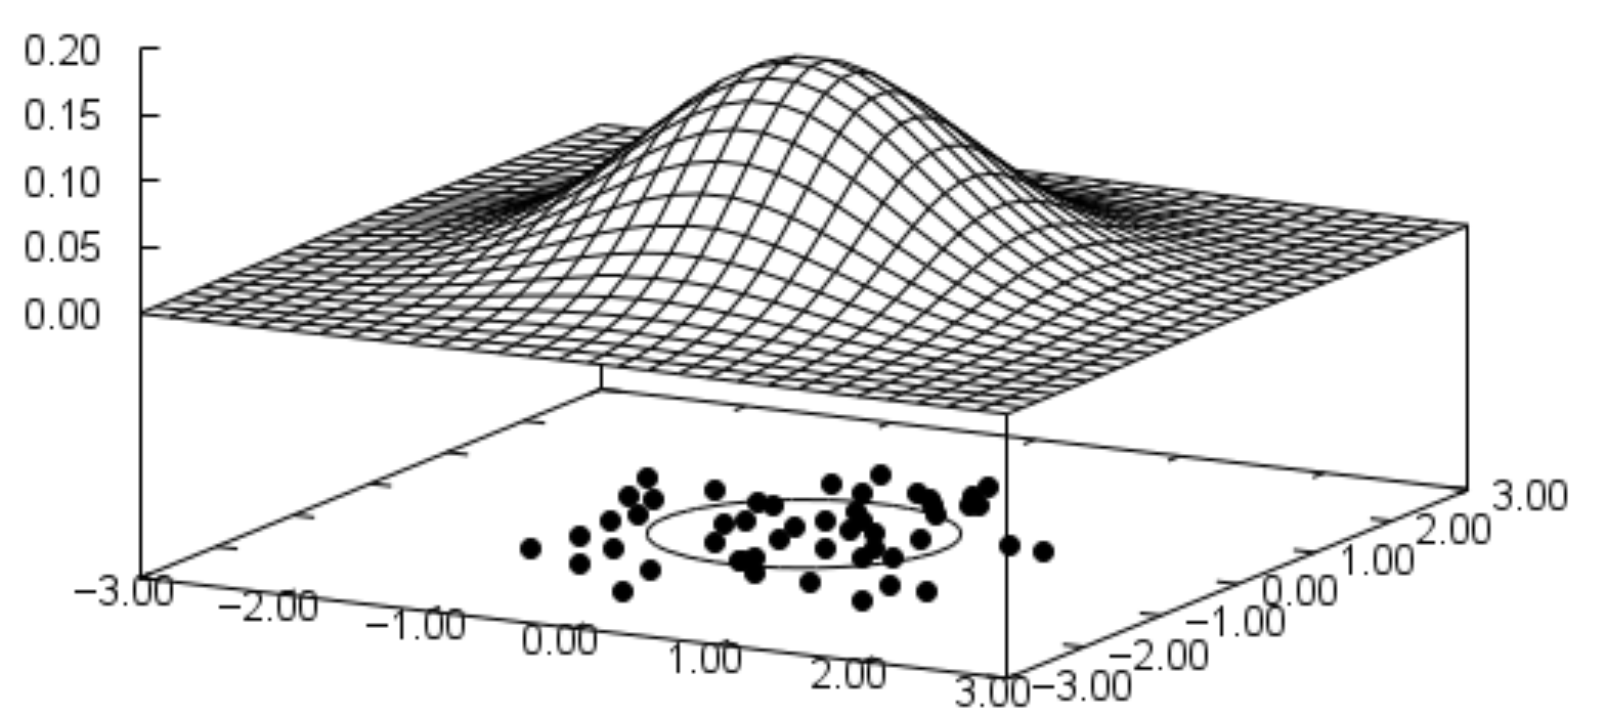
\includegraphics[scale=0.4]{img/gaussian}
\caption{Example of multinomial Gaussian.}
\label{gaussianfig}
\end{figure}

In figure \ref{posteriorApprox} the Laplace approximation of the posterior (darker lines) is shown while the lighter lines are the true unnormalised posterior. The centre point corresponds to the maximum point $\hbe$. Note how the approximation is good around $\hbe$ and it diverges going further from it.
\begin{figure}
\centering
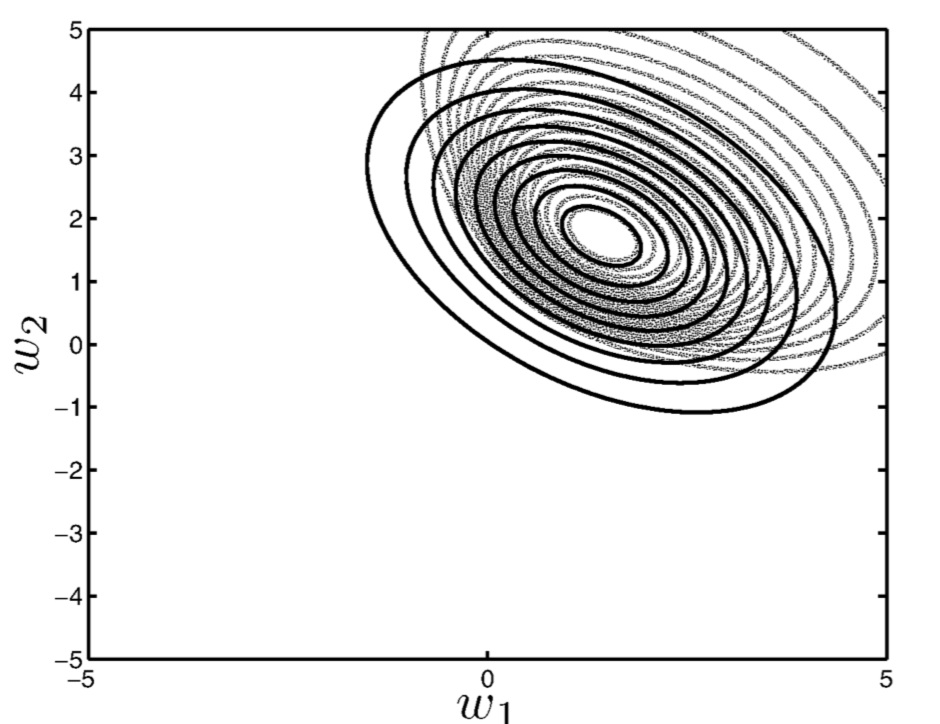
\includegraphics[scale=0.4]{img/posteriorApprox}
\caption{The axis are the parameters. The Laplace approximation of the posterior (darker lines) is shown while the lighter lines are the true unnormalised posterior. The centre point corresponds to the maximum point $\hbe$.}
\label{posteriorApprox}
\end{figure}

We use the approximate posterior to compute predictions. But now we have a density and not a single value: the prediction is computed by averaging over this density: it is like averaging over all possible values of $\be$. We should calculate the expected value $Pr(Y_{new} = 1|\x_{new}, \be)$ with respect to the approximate posterior denoted as $\CMcal{N}(\mathbf{\mu, \Sigma})$:
\begin{equation}
Pr(Y_{new}=1|\x_{new}, \X, \be) = \E_{\CMcal{N}(\mathbf{\mu, \Sigma})}\left\lbrace Pr(T_{new}=1| \x_{new}, \be)\right\rbrace
\end{equation}
However, we cannot compute the integral (of the expectation), but we can sample from $\CMcal{N}(\mathbf{\mu, \Sigma})$ and approximate the expectation with a sum:
\begin{equation}
\label{approxDen}
Pr(Y_{new}=1|\x_{new}, \X, \be) = \frac{1}{N_s}\sum_{s=1}^{N_s}\frac{1}{1+e^{-\be_s^T \x_{new}}}
\end{equation}

\paragraph{\textbf{Comparison between the decision boundaries of MAP and Laplace method.}} In case of MAP estimation we get a single separating line as in \ref{MAP1} for the example of two classes. In case of Laplace approximation we don't have a single separating line but a density distribution. \ref{laplace1} shows 20 boundaries (i.e., set of coefficients) sampled randomly from the distribution. All or almost all separates the classes quite well but in the area from the graph further from the classes (or from the centroids or clusters) there is a lot of variability. This variability represents the uncertainty of the classifier in those area far from the classes, where no event (in the sense of data entry) was observed.

This is made clearer by looking at the decision boundaries in \ref{MAP2} and \ref{laplace2}. In case of MAP it is quite obvious: the probability increases or decreases just moving close to or far from to the boundary. In case of Laplace approximation the contours are no longer straight lines. The probability are now close to $0.5$ in all the area except those closes to the two classes. It is like the classifier is unable to take a decision in those areas, that are the ones where no event has been noted.

On the contrary the classifier resulting from MAP approximation is always sure about its work: it can only classify either with one or the other class except in on the points on the boundaries. This result from the fact that it is the result of a single point and not a distribution: i.e., the amount of confidence on the result is left out.

\begin{figure}
\begin{subfigure}[t]{0.5\textwidth}
\centering
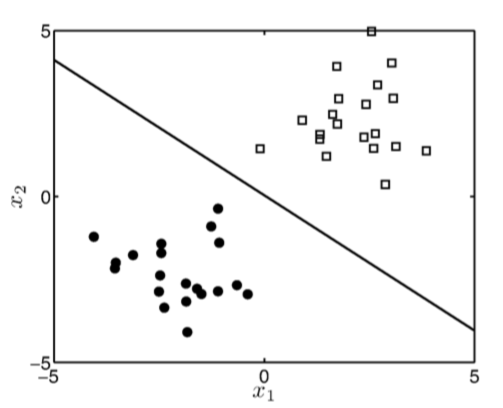
\includegraphics[width=0.85\linewidth]{img/MAP1}
\caption{Decision boundary for MAP estimation.}
\label{MAP1}
\end{subfigure}
\hfill
\begin{subfigure}[t]{0.505\textwidth}
\centering
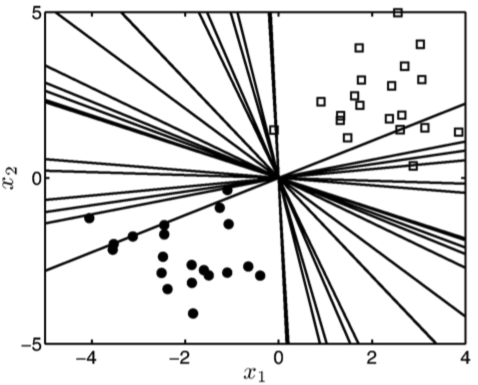
\includegraphics[width=0.8\linewidth]{img/laplace1}
\caption{Decision boundary for Laplace approximation estimation.}
\label{laplace1}
\end{subfigure}
\begin{subfigure}[t]{0.5\textwidth}
\centering
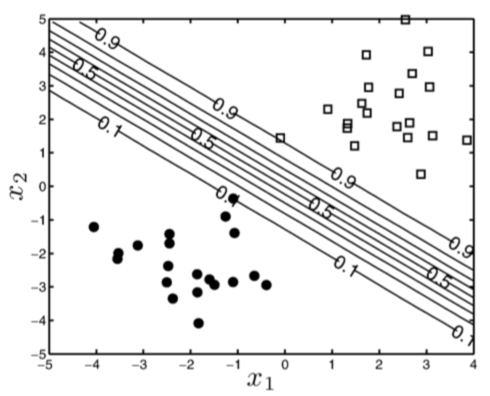
\includegraphics[width=0.8\linewidth]{img/MAP2}
\caption{Contours of probability of belonging to class 1 in case of MAP estimation.}
\label{MAP2}
\end{subfigure}
\hfill
\begin{subfigure}[t]{0.5\textwidth}
\centering
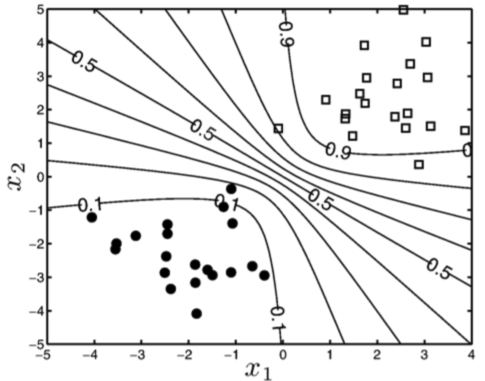
\includegraphics[width=0.8\linewidth]{img/laplace2}
\caption{Contours of probability of belonging to class 1 in case of Laplace approximation estimation computed with a sample based approximation.}
\label{laplace2}
\end{subfigure}
\caption{Comparison between MAP and Laplace approximation contours and probability densities.}
\end{figure}

\subsubsection{Third method: sampling technique	}
The reason of estimating the posterior density with Laplace approximation or any other method is to take into account uncertainties in $\be$ when making predictions. Using the Gaussian approximation we were able to sample as in equation \ref{approxDen} directly from data. When deciding we take the conditional probability by averaging all over the potential values $\be$ by taking the expectation:
\begin{equation}
Pr(T_{new}=1| x_{new}, \X, \y, \sigma^2) = \E_{Pr(\be|\X, \y, \sigma^2)}\br{Pr(T_{new}=1|x_{new},\be}
\end{equation}

In these types of approximations we cut off the approximation step and sample directly from the posterior. A set of samples from the true posterior could be substituted directly into equation \ref{approxDen} to compute the desired predictive probability $Pr(y_i|\x_i, \X, \be)$. A popular sampling technique is the \textbf{Metropolis-Hastings} algorithm.

Drawing from the posterior does not mean we can write it down but that we sample directly the system (physical or whatever) generating the data.

\paragraph{The metropolis-Hastings algorithms}
The objective is to sample from $Pr(\be|\X,\y,\sigma^2)$ to approximate the following expectation:
\begin{equation}
\begin{aligned}
Pr(Y_{new}&=1|x_{new},\X,\y,\sigma^2) = \E_{Pr(\be|\X,\y,\sigma^2)}\left[Pr(T_{new}=1|x_{new},\be) \right] \\
&=\int Pr(Y_{new}=1|x_{new},\be)Pr(\be|\X,\y,\sigma^2) d\be
\end{aligned}
\end{equation}
with 

\begin{equation}
\begin{aligned}
Pr(Y_{new}&=1|x_{new},\X,\y,\sigma^2) \approx \frac{1}{N_s}\sum_{s=1}^{N_s} Pr(Y_{new}=1|x_{new}, \be_s)
\end{aligned}
\end{equation}
The algorithm generates a sequence of samples $\be_1, \be_2, \cdots$. First all the algorithm is independent from the starting point, as long as we sample long enough: it is guaranteed the sequence converges.
\paragraph{\textbf{The generation of new samples}} happens in this way. Suppose we have the sample $s-1$, we will propose a new sample $\tilde{\be_s}$ and define the density $Pr(\tilde{\be}_s|\be_{s-1})$. This density is unrelated with the posterior $Pr(\be|\X,\y,\sigma^2)$ and we can define it as we please but it will affect the convergence time. A common choice is to use a Gaussian centred on the current sample, $\be_{s-1}$:
\begin{equation}
Pr(\tilde{\be}_s|\be_{s-1}, \Sigma) =\CMcal{N}(\be_{s-1}, \Sigma)
\end{equation}
Generally $\sigma$ is taken diagonal with same values. The smaller the elements on the diagonal, the smaller the distance at each step.

Such a sequence creates a \textbf{random walk}. The choice of the Gaussian is justified bye the easy of sampling from the Gaussian and by its symmetry: moving from $\tilde{\be}_{s-1}$ to $\tilde{\be}_s$ is just as likely to move from $\tilde{\be}_s$ to $\tilde{\be}_{s-1}$:
\begin{equation}
Pr(\tilde{\be}_s|\be_{s-1}, \Sigma)  = Pr(\tilde{\be}_{s-1}|\be_{s}, \Sigma) 
\end{equation}
\textbf{Accepting or rejecting the candidate $\tilde{\be}_s$} is performed by calculating the following quantity:
\begin{equation}
r = \frac{Pr(\tilde{\be}_s|\X, \y, \ssq)}{Pr(\be_{s-1}|\X, \y, \ssq)}\frac{Pr(\be_{s-1}|\tilde{\be}_s, \Sigma)}{Pr(\hat{\be}_{s}|\be_{s-1}, \Sigma)}
\end{equation}
The expression is the product of the ratio of the posterior density at the proposed sample to that at the old sample times the ratio of the proposed densities. For the Gaussian symmetry discussed above, this term is $1$ when using Gaussian densities. Note that we cannot compute exactly the densities, but being a ratio the normalisation constant (the denominator in Bayes expression) simplifies and only the likelihoods times the priors are left:
\begin{equation}
r = \frac{Pr(\tilde{\be}_s|\ssq)}{Pr(\be_{s-1}| \ssq)} \frac{Pr(\y|\X, \tilde{\be}_s, \ssq)}{Pr(\y|\X, \be_{s-1}, \ssq)}
\end{equation}
If $r>1$, i.e, we get a higher posterior density, we accept the candidate otherwise we accept the candidate with probability equal to $r$. The complete algorithm is depicted in \ref{MHAlgo} where a uniform distribution in $[0,1]$ is used as decision rule in case $r<1$. Being a uniform distribution, the probability that $u \le r$ is $r$.

\begin{figure}
\centering
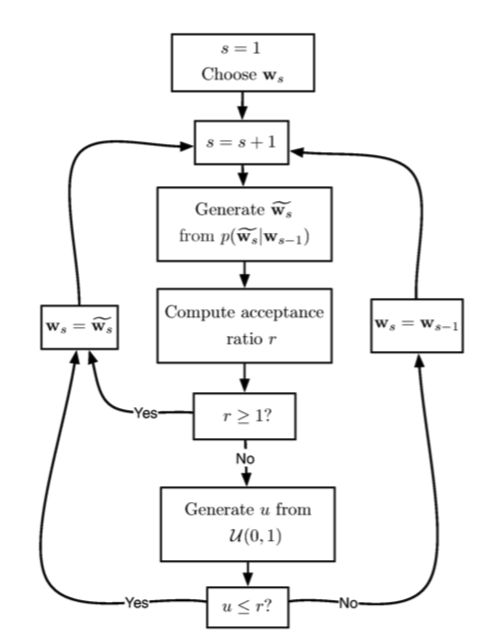
\includegraphics[scale=0.45]{img/MHAlgo}
\caption{The steps of the Metropolis-Hastings algorithm. $U$ is a uniform distribution in $[0,1]$}
\label{MHAlgo}
\end{figure}

\ref{randomWalk} shows a 10-iteration process of the algorithms where solid lines are accepted coefficients, dashed lines are the rejected ones. Note that even the third sample causes a decrease in the posterior $r<1$, nevertheless in this specific case the decision rule accepted it. On the contrary the 4-th sample causes a huge decrease hence it is very unlikely it is accepted and in fact it is not, so $\be_4 = \be_3$. After $N$ samples we compute the sample based approximations to the mean and covariance
\begin{equation}
\begin{aligned}
\mu' &= \frac{1}{N_s} \sum_{s=1}^{N_s} \be_s\\
S' &= \frac{1}{N_s} \sum_{s=1}^{N_s} (\be_s-\mu')(\be_s-\mu')^T
\end{aligned}
\end{equation}

\begin{figure}
\centering
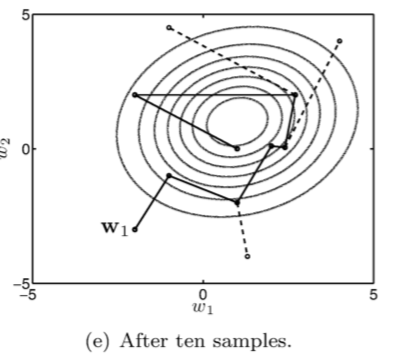
\includegraphics[scale=0.4]{img/randomWalk}
\caption{Example of Metropolis-Hastings iterations: solid lines are accepted coefficients, dashed lines are the rejected ones.}
\label{randomWalk}
\end{figure}

\begin{definition}{\textbf{Burn-in}} It is the time interval between the starting of the algorithm and the convergence. 
\end{definition}
It cannot be determined: to overcome this problem, a method for determining convergence (to a distribution, not to a value) should be established. For example, in the algorithm above, we do not know if the starting point belongs to an area from which we are supposed to sample: it might be very far from the posterior. Including these samples in the approximation might result in a not good value. That is why the first samples (ranging from few samples to thousands) should be discarded.

A popular method is to start several samplers simultaneously from different starting points. When all the samplers are generating samples with similar mean and variance, it suggests they converged all to the same distributions.

\begin{definition}{\textbf{convergence} In this case we are talking about the convergence to a given distribution, not a single point. The convergence to a distribution is characterized to the convergence of its parameters: in case of the Gaussian the mean and variance.}
\end{definition}

We can even look at each coefficient independently:
\begin{equation}
Pr(\be_1|\X,\y,\sigma^2) = \int Pr(\be_1,\be_2|\X,\y,\sigma^2) d\be_2
\end{equation}

\paragraph{\textbf{To calculate the predictive probability}} using the obtained set of samples, we can do what already done with the Laplace approximation:
\begin{equation}
Pr(Y_{new}=1|\x_{new}, \X,\y,\sigma^2) = \frac{1}{N_s} \sum_{s=1}^{N_s} \frac{1}{1+e^{-\be^T_s \x_{new}}}
\end{equation}

\begin{figure}
\begin{subfigure}{.47\textwidth}
\centering
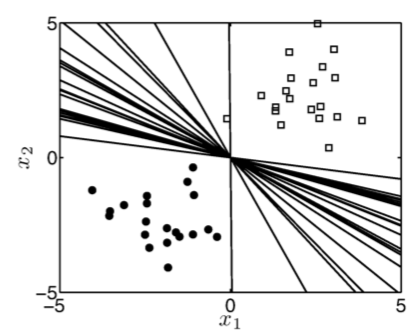
\includegraphics[width=.8\linewidth]{img/MH1}
\caption{Predictive probability contours of classifying objects as square.}
\label{MH1}
\end{subfigure}
\begin{subfigure}{.47\textwidth}
\centering
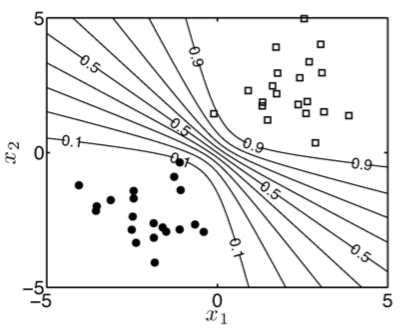
\includegraphics[width=.8\linewidth]{img/MH2}
\caption{Decision boundaries created from randomly selected MH samples.}
\label{MH2}
\end{subfigure}
\caption{Example of Metropolis-Hastings algorithm results.}
\end{figure}
\ref{MH1} and \ref{MH2} show an example of possible shapes of contours: it does not look too different from the Laplace ones. The only difference is that these contours are not so tight as the Laplace's ones. This suggests the probability decreases more slowly.

\paragraph{\textbf{Limitations}} The difficult mostly lies in the unknown shape of the density. When a density has two or more modes, MH moves towards the modes as these moves increase the posterior density and hence are always accepted. When close to a mode, many steps are required to move from one mode to another and this is very unlikely. We might end up exploring a mode without even knowing the other exists (see \ref{mode1}). Another problem arises when the variables are strongly correlated (see \ref{mode2}). Let us pick any position and propose a movement from a Gaussian with diagonal covariance (i.e., having circular contours). The shapes are very different and many samples will be rejected: the majority of moves that we sample from our proposal will involve moving steeply down the probability gradient. There are even other problems.

\begin{figure}
\begin{subfigure}{.5\textwidth}
\centering
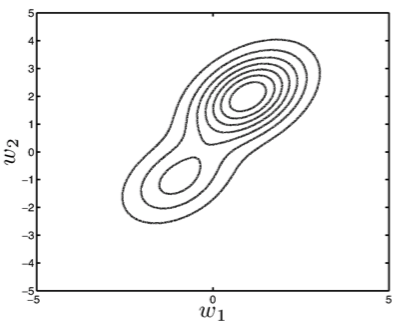
\includegraphics[width=.8\linewidth]{img/mode1}
\caption{A bi-modal density.}
\label{mode1}
\end{subfigure}
\begin{subfigure}{.5\textwidth}
\centering
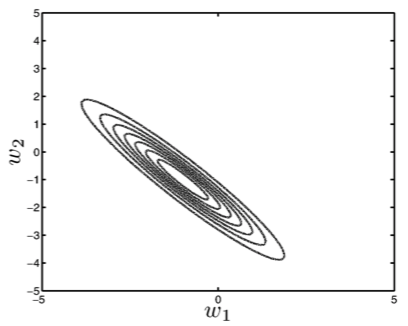
\includegraphics[width=.8\linewidth]{img/mode2}
\caption{Highly correlated parameter density.}
\label{mode2}
\end{subfigure}
\caption{Example of Metropolis-Hastings algorithm results.}
\end{figure}

\subsubsection{Usage}
LR is used as data analysis tool where the goal is to  understand the role of the input variables in explaining the outcome. Typically many models are fit in a search for a parsimonious model involving a subset of the variables, possibly with some interactions terms. 

It is widely used in biostatistical applications where binary responses (two classes) occur quite frequently. For example, patients survive or die, have heart disease or not, or a condition is present or absent.
\subsection{Regularized Logistic regression}
We can use the $L_1$ penalty for variable selection and shrinkage:

\begin{equation}
\argmax{\beta_0,\beta_1} \left\lbrace \sum_{i=1}^N y_i\left(  \beta_0 + \beta^Tx_i\right) -\log \left( 1+e^{\beta_0 + \beta^T x_i}\right) -\lambda \sum_{j=-1}^p |\beta_j|\right\rbrace
\end{equation}
This function is concave and can be solved using a nonlinear programming method.
\subsection{Logistic vs LDA}
The difference between the models relies on how the linear coefficients are estimated. The logistic regression model is more general since it makes less assumptions.

LDA is not robust to outliers since observations far from the decision boundary are used to estimate the common covariance matrix, while they are scaled down in the Logistic regression.

\subsection{Perceptron learning algorithm}
It tries to find a separate hyperplane by minimizing the distance of misclassified points to the decision boundary. If a response $y_i = 1$ is misclassified, then $x^T_i \beta + \beta_0 < 0$, and the opposite for a misclassified response with $y_i = -1$. The goal is to minimize
\begin{equation}
D(\beta, \beta_0) = - \sum_{i\in\CMcal{M}} y_i\left(x_i^T\beta + \beta_0\right)
\end{equation}
where $\CMcal{M}$ is the set of misclassified points.
The gradient is
\begin{align}
\frac{\partial D(\beta,\beta_0}{\partial \beta} = -\sum_{i\in\CMcal{M}}y_ix_i \\
\frac{\partial D(\beta,\beta_0}{\partial \beta_0} = -\sum_{i\in\CMcal{M}} y_i
\end{align}
where the algorithm uses the stochastic gradient descent where the coefficients are updated by the gradient value weighted by a step $\rho$. There are many problems though:
\begin{itemize}
\item when data are separable, there are many solutions which depend on the starting value;
\item many steps might be required;
\item when data are not separable, the algorithm will not converge;
\end{itemize}
\subsection{Optimal separating hyperplanes}
The optimal separating hyperplane separates the two classes and maximizes the distance to the closest point from either class (Vapnik, 1996). Not only does this provide a unique solution to the separating hyperplane problem, but by maximizing the margin between the two classes on the training data, this leads to better classification performance on test data.

Suppose $M$ is the distance. Then
\begin{equation}
\begin{aligned}
&\max\limits_{\beta,\beta_0, ||\beta||=1} M \\
& y_i(x_i^T\beta + \beta_0) \ge M
\end{aligned}
\end{equation}
We  can move the constrain on the module $\||\be||=1$ to the condition $\frac{1}{||\be||}y_i(x_i^T\beta + \beta_0) \ge M$, which redefines $\be_0$. 

For a pair of coefficients satisfying this inequalities, any positively scaled multiple satisfies them too, so we can set arbitrarily set $||\be||=\frac{1}{M}$:
\begin{equation}
\begin{aligned}
&\min_{\be, \be_0}{\frac{1}{2}||\be||^2}\\
\textit{subject to } &y_i(x_i^T\be+\be_0)\ge1
\end{aligned}
\end{equation}

With this constraint, a margin around the decision boundary with thick $\frac{1}{||\be||}$ is present. We choose $\be$ to maximize the thickness of margin margin.  This is a convex optimization problem. The Lagrange primal function to be minimized is:
\begin{equation}
\label{eq}
L_p = \frac{1}{2} ||\be||^2 = \sum_{i=1}^N \alpha_i\left[ y_i \br{x_i^T\be+\be_0}\right]
\end{equation}
and setting the derivatives to $0$:
\begin{equation}
\begin{aligned}
\be &= \sum_{i=1}^N \alpha_i y_i x_i
0  &= \sum_{i=1}^N \alpha_i y_i
\end{aligned}
\end{equation}
and substituting in \ref{eq}:
\begin{equation}
\begin{aligned}
L_D = \sum_{i=1}^N \alpha_i -\frac{1}{2}\sum_{i=1}^N\sum_{k=1}^N \alpha_i \alpha_ky_iy_kx_i^Tx_k\\
\textit{subject to } \alpha_i\ge0 \textit{ and } \sum_{i=1}^N \alpha_iy_i=0
\end{aligned}
\end{equation}
The optimal hyperplane focuses more on points that counts, i.e., close to the border. For this reason it is more robust. LDA depends on all the data, even points faraway. If classes are really Gaussian LDA is optimal and separating hyperplane will pay a price for focusing on noisier data.
For logistic regression, if a separate hyperplane exists, since the log-likelihood can be driven to $0$.

When data are not separable there will be no feasible solution and an alternative formulation is needed.

\section{Basis expansion and regularization}
To extend the flexibility of linear model, a transformation of $\X$ can be performed and then use a linear model to the derived input features. Denoting the transformation $h_m(\X) : \CMcal{R}^p\rightarrow \CMcal	{R}$ for a single input $m$, we have the model:
\begin{equation}
f(\X) = \sum_{m=1}^M \beta_mh_m(\X)
\end{equation}
$h()$ are called \textbf{basis function}
Any kind of transformation can be applied: square-roots, squared (on single inputs i.e, $x_i^2$ or among different inputs $x_ix_j$), logarithmic, power functions, trigonometric, etc. 

Polynomials are more widely used but they have a limitation due to its global nature: when tweaking the  parameters to achieve a desired behaviour in a specific region, problems might arise in another region.

A solution is to consider \textbf{piecewise-polynomials} and \textbf{splines}.

\subsection{Piecewise Polynomials and splines}
For the moment $X$ is assumed one-dimensional. A piecewise polynomial function is obtained by  dividing the domain of $X$ into contiguous intervals and use a different $f$ in each interval.

Given a sequence $a=t_0<t_1<\cdots<t_{m+1}=b$, the piecewise polynomials are delimited by an adjacent pair in the sequence. So we have the following sequence of intervals:

\begin{equation}
I_l = \left[ t_{l-1}, t_l\right) \textit{ for } 1\le l\le m \textit{ and } \left[t_m, t_{m+1}\right]
\end{equation}
So the piecewise polynomials, having basis functions: $h_0(X) = 1, h_1(X) = X, h_2(X) = X^2$ and so on, is:

\begin{equation}
f(x) = \left\{ \begin{array}{ll} g_0(x) = \beta_{0,0} + \beta_{0,1} X + \cdots + \beta_{0,k-1} X^{k-1}\quad X \in I_1 \\ 
\vdots\\
 g_{m-1}(x) = \beta_{m-1,0} + \beta_{m-1,1} X + \cdots + \beta_{m-1,k-1} X^{k-1}\quad X \in I_{k+1} \\  \quad 
\end{array}
 \right.
\end{equation}

In this way we get discontinuities at the boundaries. Note that discontinuity means we get completely different values for almost the same input. More often we would like to have continuity at the boundaries or knots: $f(\xi^+)=f(\xi^-)$ which implies the condition:$\beta_1 +\xi\beta_2 = \beta_3 +\xi_1\beta_4$ which removes one degree of freedom.

These constrains, one for each knot, can be embedded in additional basis functions of the type $h(X) = \br{X - \xi}_+$ where $\br{\cdot}_+ = \max(\cdot, 0)$ i.e., the basis function is $0$ for $X - \xi<\xi$, $X - \xi$ otherwise
\begin{equation}
h(X) = \br{X - \xi}_+ = \max(X - \xi, 0) = \left\{ \begin{array}{ll}  0 &\quad X-\xi<0\\
X-\xi &\quad X-\xi\ge0
\end{array}
 \right.
\end{equation}

Using the previous and these basis functions we can reexpress the global function as:
\begin{equation}
\begin{aligned}
f(x) =& \beta_{0,0} + \beta_{0,1}X +\cdots+\beta_{0,k-1}  X^{k-1} + \\
&+\beta_{1,0}(X -\xi_0)_+^0     + \beta_{1,1}(X -\xi_0)_+^1       +\cdots +\beta_{1,k-1} (X -\xi_0)_+^{k-1}+  \\
&+\vdots \\ 
&+\beta_{m-1,0}(X -\xi_{m-1})_+^0 +\cdots +\beta_{m-1,k-1} (X -\xi_{m-2})_+^{k-1}
\end{aligned}
\end{equation}
\textbf{To force continuity between two regions} we set the terms $\beta_{1,0}(X -\xi_j)_+^0$ to $0$:

For example forcing continuity at the first knot:
\begin{equation}
\begin{aligned}
&\beta_{1,0}(X -\xi_0)_+^0 = \beta_{0,0} + \beta_{0,1} \xi_0\\
&\Rightarrow \beta_{1,0} = \beta_{0,0} + \beta_{0,1} \xi_0
\end{aligned}
\end{equation}

 In this way we don't have a jump at the boundaries:

\begin{equation}
\begin{aligned}
f(x) =& \beta_{0,0} + \beta_{0,1}X +\cdots+\beta_{0,k-1}  X^{k-1} + \\
&+ \beta_{1,1}(X -\xi_0)_+^1       +\cdots +\beta_{1,k-1} (X -\xi_0)_+^{k-1}+  \\
&+\vdots \\ 
&+ \beta_{m-1,1}(X -\xi_{m-1})_+^1 +\cdots +\beta_{m-1,k-1} (X -\xi_{m-1})_+^{k-1}
\end{aligned}
\end{equation}
In this way we have removed $m-1$ parameters.

There is a difference in this representation: before we have to select a polynomial function for a specific region where the fit to the global function was given by the fit of the parameters specific to that region, now we have a global function that works a little differently. In the first region, the only non-null terms are $\beta_{0,j}$ as before. When reaching the second region, the terms $\beta_{1,j}$ becomes non-null. Now the coefficients of the polynomial are the sum of the coefficients of these two region: i.e., in the second region we have:
\begin{equation}
\begin{aligned}
f(x) =& \beta_{0,0} -(\beta_{1,1}+\cdots+\beta_{1,k-1})\xi_0+ (\beta_{0,1}+\beta_{1,1})X+\\
&+\cdots+(\beta_{0,k-1}  +\beta_{1,k-1})X^{k-1}
\end{aligned}
\end{equation}

\ref{spline_linear} shows the global function, solid line, given by the sum of basis functions, dashed lines, when traversing the graph from left to right. At each knot, a new basis function is activated and summed to the global function.

The basis functions can be seen as a correction to the global polynomial for that  specifc region and the knots are those points where the correction starts. At the knot $X=\xi_j$ so the correction starts very gently and the continuity is preserved.

\begin{figure}
\begin{subfigure}{0.49\textwidth}
\centering
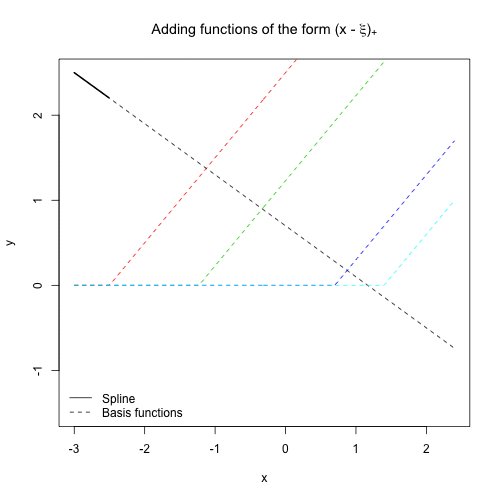
\includegraphics[width=0.9\linewidth]{img/spline_linear/10}
\caption{First region.}
\end{subfigure}
\hfill
\begin{subfigure}{0.49\textwidth}
\centering
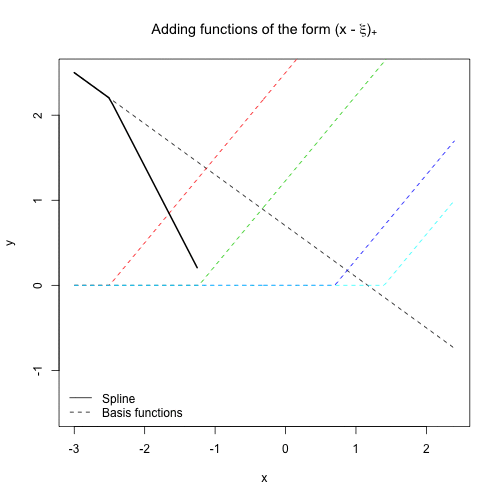
\includegraphics[width=0.9\linewidth]{img/spline_linear/33}
\caption{Second region.}
\end{subfigure}
\begin{subfigure}{0.49\textwidth}
\centering
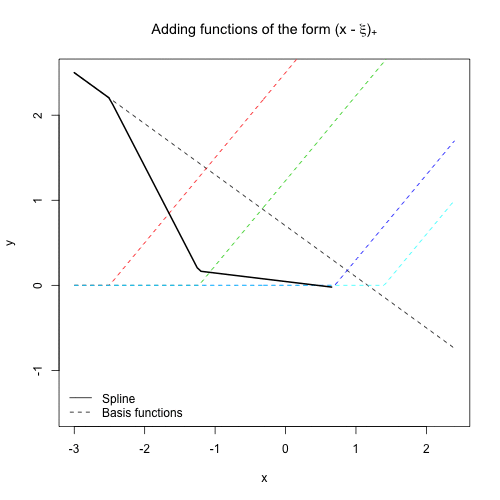
\includegraphics[width=0.9\linewidth]{img/spline_linear/68}
\caption{Third region.}
\end{subfigure}
\hfill
\begin{subfigure}{0.49\textwidth}
\centering
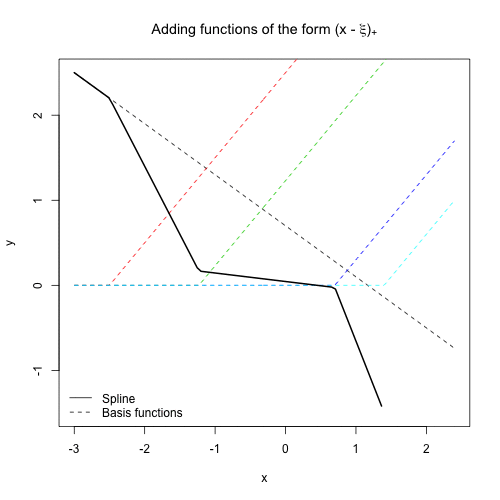
\includegraphics[width=1\linewidth]{img/spline_linear/81}
\caption{Fourth region.}
\end{subfigure}
\end{figure}
\begin{figure}\ContinuedFloat
\begin{subfigure}{0.49\textwidth}
\centering
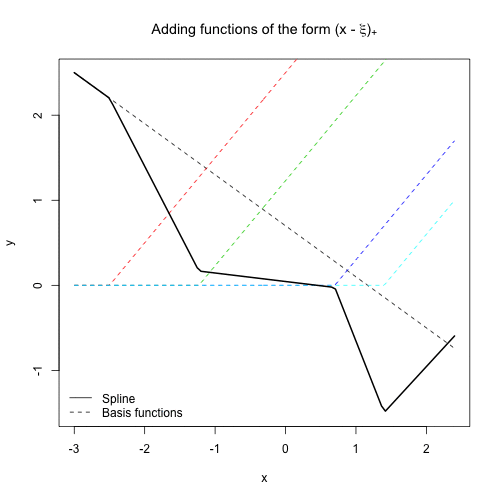
\includegraphics[width=1\linewidth]{img/spline_linear/100}
\caption{Fifth region.}
\end{subfigure}
\caption{Linear splines. The solid line is the global function while the dashed lines are the basis functions.}
\label{spline_linear}
\end{figure}

Generally, smoother functions are preferred and these are achieved by increasing the order of the local polynomials and increasing the order of continuity (continuity first derivative, second derivative). It is claimed that cubic splines are the lowest-order spline for which the discontinuity is not visible to the human eye and seldom higher degrees are needed, unless smooth derivatives are required.

The spline order, number of knots and their positions must be selected. Generally the position of the knots is chosen according the observation, while the order is chosen a-priori.

\begin{figure}
\begin{subfigure}{0.49\textwidth}
\centering
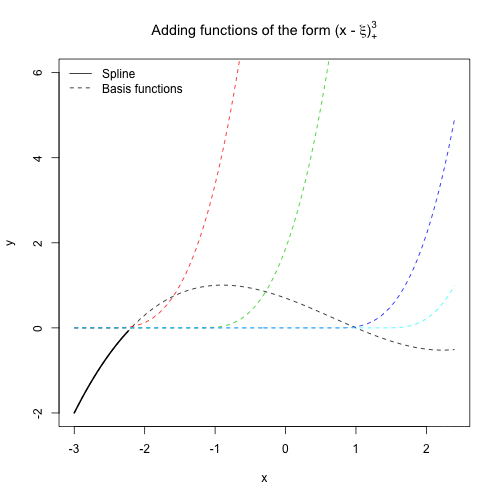
\includegraphics[width=1\linewidth]{img/spline_cubic/15}
\caption{First region.}
\end{subfigure}
\hfill
\begin{subfigure}{0.49\textwidth}
\centering
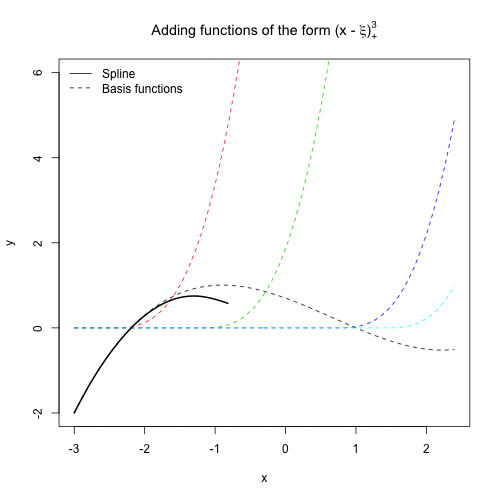
\includegraphics[width=1\linewidth]{img/spline_cubic/41}
\caption{Second region.}
\end{subfigure}
\begin{subfigure}{0.49\textwidth}
\centering
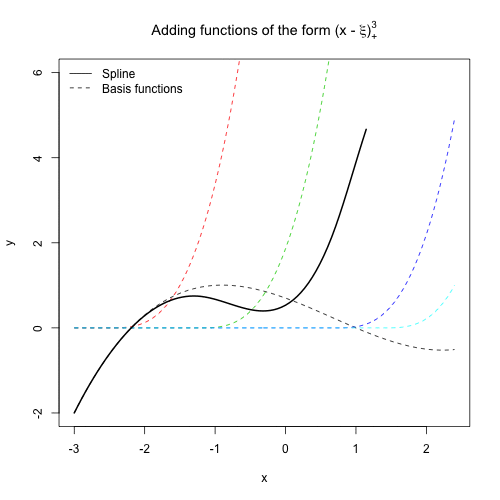
\includegraphics[width=1\linewidth]{img/spline_cubic/77}
\caption{Third region.}
\end{subfigure}
\hfill
\begin{subfigure}{0.49\textwidth}
\centering
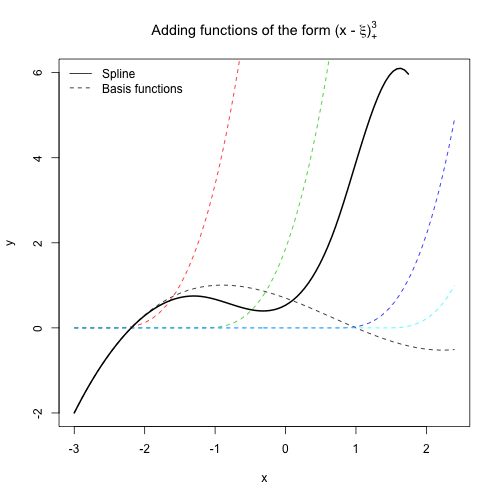
\includegraphics[width=1\linewidth]{img/spline_cubic/88}
\caption{Fourth region.}
\end{subfigure}
\end{figure}
\begin{figure}\ContinuedFloat
\begin{subfigure}{0.49\textwidth}
\centering
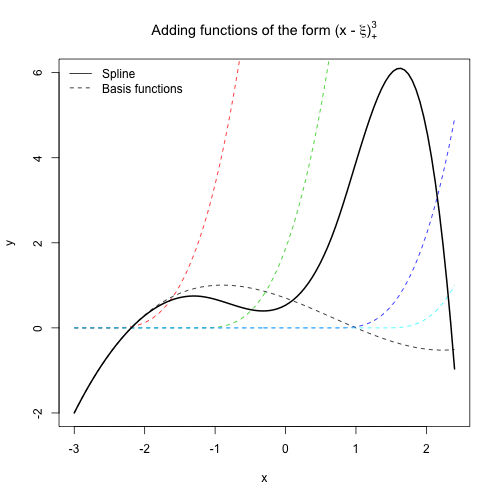
\includegraphics[width=1\linewidth]{img/spline_cubic/100}
\caption{Fifth region.}
\end{subfigure}
\label{spline_cubic}
\caption{Cubic splines. The solid line is the global function while the dashed lines are the basis functions.}
\end{figure}

\subsection{Natural cubic splines}
Polynomial fits to data tends to be erratic at the boundaries and additionally splines behave even more widely than the global polynomial beyond the boundaries. This is shown by the point-wise variance (the variance of the estimator at one point: $\Var[\hat{f}(x_0)]$ in \ref{pointwise_var}. Note the variance explosion close to the boundaries, especially for cubic splines.

\begin{figure}
\centering
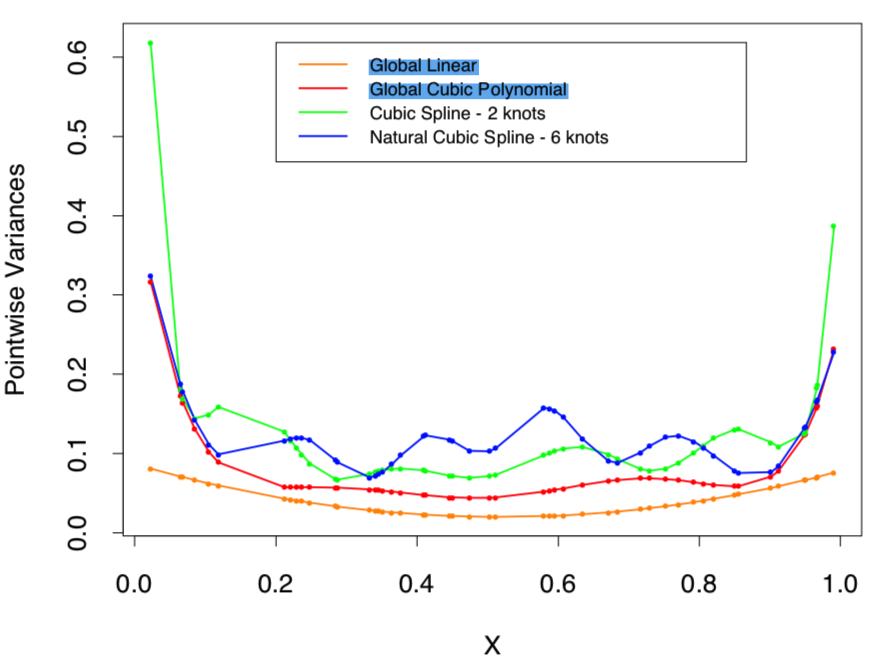
\includegraphics[scale=0.4]{img/pointwise_var}
\caption{$X$ consists of 50 points drawn randomly from $U[0,1]$ and an assumed error model of with constant variance. Both cubic splines have 6 degrees of freedom. The cubic spline has two knots at $0.33$ and at $0.66$ while the natural cubic spline has boundary knots at $0.1$ and $0.9$, and four interior knots uniformly spaced between them.}
\label{pointwise_var}
\end{figure}

A  \textbf{natural cubic spline} adds additional constraints by forcing linearity beyond the boundary knots. These frees up four degrees of freedom (2 in both boundary regions), that can be used more profitably by sprinkling more knots in the interior region. There will be a price to pay in terms of bias near the boundaries, but in these regions we have less information anyway so assuming the function is linear here is reasonable.

A natural cubic spline with $K$ knots is represented by $K$ basis functions. One can start from the basis of a cubic spline and then derive the reduce basis by imposing the boundary constraints.

Starting from the general continuous basis for four regions (four knots):
\begin{equation}
\begin{aligned}
&h_1(X) =1, \quad\quad\quad h_2(X) =X,\quad h_3(X) =X^2,\quad  h_4(X) = X^3,\\
&h_5(X) = X-\xi_0,\quad h_6(X) = (X-\xi_0)^2,\quad, h_7(X) = (X-\xi_0)^3\\
&h_8(X) = X-\xi_1,\quad h_9(X) = (X-\xi_1)^2,\quad h_{10}(X) = (X-\xi_1)^3\\
&h_9(X) = X-\xi_2,\quad h_10(X) = (X-\xi_1)^2,\quad h_{11}(X) = (X-\xi_2)^3
\end{aligned}
\end{equation}
Enforcing also continuity of the first and second derivatives at the knots we reduce the basis to:
\begin{equation}
\begin{aligned}
&h_1(X) = 1, \quad h_2(X) =X,\quad h_3(X) =X^2,\quad  h_4(X) = X^3,\\
&h_5(X) = (X-\xi_0)^3, \quad h_6(X) = (X-\xi_1)^3, \quad h_7(X) = (X-\xi_2)^3.
\end{aligned}
\end{equation}

Enforcing linearity beyond the boundaries, we eliminate $ h_3(X)$ and $ h_4(X)$. We must also keep the cubic expression in the intermediate regions but somehow make the cubic part cancel out when reaching the fifth region since here it must be linear. We can add for each region in the interval $[1, K-2]$ the following basis function:
\begin{equation}
\begin{aligned}
&h_k(X) = d_k(X) - d_{K-1}(X)\\
\textit{where} \quad &d_k(X) = \frac{\br{X-\xi_k}_+^3 - \br{X-\xi_K}_+^3 }{\xi_K - \xi_k}
\end{aligned}
\end{equation}

In the first region we have:
\begin{equation}
\hat{f}_1(X) = \beta_0 + \beta_1 X
\end{equation}
In the second region we have:
\begin{equation}
\begin{aligned}
&\hat{f}_2(X) = \beta_0 + \beta_1 X +\beta_2 \frac{(X-\xi_0)^3}{\xi_2 - \xi_0} =\\
&= \beta_0 + \beta_1 X +\beta_2 \frac{X^3 -3 \xi_0 X^2 + 3\xi_0^2 X-\xi_0^3}{\xi_2 - \xi_0} =\\
&= \frac{\beta_2}{\xi_2 - \xi_0} X^3 -3 \beta_2\frac{\xi_0}{\xi_2 - \xi_0} X^2 + (\beta_1+3\beta_2\frac{\xi_0^2}{\xi_2 - \xi_0})X + \beta_0 - \beta_2\frac{\xi_0^3}{\xi_2 - \xi_0}
\end{aligned}
\end{equation}
In the third region we have:
\begin{equation}
\begin{aligned}
&\hat{f}_3(X) = \beta_0 + \beta_1 X  +\beta_2 h_2(X) = \beta_0 + \beta_1 X  +\beta_2\left[ \frac{(X-\xi_0)^3}{\xi_2 - \xi_0} - \frac{(X-\xi_1)^3}{\xi_2 - \xi_1}\right]  \\
&= \beta_0 + \beta_1 X +\beta_2 \left[ \frac{X^3 -3 \xi_0 X^2 + 3\xi_0^2 X-\xi_0^3}{\xi_2 - \xi_0} -  \frac{X^3 -3 \xi_1 X^2 + 3\xi_1^2 X-\xi_1^3}{\xi_2 - \xi_1}\right] =\\
&= \beta_0 + \beta_1 X +\beta_2 \frac{(\xi_2-\xi_1-\xi_2+\xi_0)X^3-3\left[ \xi_0(\xi_2-\xi_1) - \xi_1(\xi_2-\xi_0)\right]X^2}{(\xi_2 - \xi_0)(\xi_2 - \xi_1)}+\\
&\quad +  \frac{3\left[\xi_0^2(\xi_2-\xi_1) - \xi_1^2(\xi_2-\xi_0) \right]X-\left[(\xi_0^3(\xi_2-\xi_1) -\xi_1^3(\xi_2-\xi_0)\right]}{(\xi_2 - \xi_0)(\xi_2 - \xi_1)}=\\
&=  \beta_0 + \beta_1 X +\beta_2 \frac{(-\xi_1+\xi_0)X^3-3\xi_2(\xi_0-\xi_1)X^2}{(\xi_2 - \xi_0)(\xi_2 - \xi_1)}+\\
&\quad +  \frac{3\left[\xi_2(\xi_0-\xi_1)(\xi_0+\xi_1)-\xi_0\xi_1(\xi_0-\xi1)\right]X}{(\xi_2 - \xi_0)(\xi_2 - \xi_1)}+\\
&\quad\quad-\frac{\left[\xi_2(\xi_0-\xi_1)(\xi_0^2-\xi_0\xi_1+\xi_1^2)-\xi_0\xi_1(\xi_0-\xi1)(\xi_0+\xi_1)\right]}{(\xi_2 - \xi_0)(\xi_2 - \xi_1)} = \\
&=\beta_0 + \beta_1 X -\beta_2 (\xi_1-\xi_0)\frac{X^3-3\xi_2X^2}{(\xi_2 - \xi_0)(\xi_2 - \xi_1)}+\\
&\quad\quad +  \frac{3\left[\xi_2(\xi_0+\xi_1)-\xi_0\xi_1\right]X-\left[\xi_2(\xi_0^2-\xi_0\xi_1+\xi_1^2)-\xi_0\xi_1(\xi_0+\xi_1)\right]}{(\xi_2 - \xi_0)(\xi_2 - \xi_1)}=\\
&= -\beta_2\frac{(\xi_1-\xi_0)}{(\xi_2 - \xi_0)(\xi_2 - \xi_1)} X^3 +3 \beta_2\frac{\xi_2(\xi_1-\xi_0)}{(\xi_2 - \xi_0)(\xi_2 - \xi_1)} X^2 + \\
&\quad\quad +(\beta_1-3\beta_2(\xi_1-\xi_0)\frac{\xi_2(\xi_0+\xi_1)-\xi_0\xi_1}{(\xi_2 - \xi_0)(\xi_2 - \xi_1)})X +\\
&\quad\quad+ \beta_0 + \beta_2(\xi_1-\xi_0)\frac{\xi_2(\xi_0^2-\xi_0\xi_1+\xi_1^2)-\xi_0\xi_1(\xi_0+\xi_1)}{(\xi_2 - \xi_0)(\xi_2 - \xi_1)}
\end{aligned}
\end{equation}
In the fourth region:
\begin{equation}
\begin{aligned}
&\hat{f}_3(X) = \beta_0 + \beta_1 X  +\beta_2 h_2(X) =\\
&= \beta_0 + \beta_1 X  +\beta_2\left[ \frac{(X-\xi_0)^3-(X-\xi_2)^3}{\xi_2 - \xi_0} - \frac{(X-\xi_1)^3-(X-\xi_2)^3}{\xi_2 - \xi_1}\right]  \\
&= \beta_0 + \beta_1 X +\beta_2 \frac{X^3 -3 \xi_0 X^2 + 3\xi_0^2 X-\xi_0^3-X^3 +3 \xi_2 X^2 - 3\xi_2^2 X+\xi_2^3}{\xi_2 - \xi_0} +\\
&\quad\quad\quad -\beta_2  \frac{X^3 -3 \xi_1 X^2 + 3\xi_1^2 X-\xi_1^3-X^3 +3 \xi_2 X^2 - 3\xi_2^2 X+\xi_2^3}{\xi_2 - \xi_1} =\\
&= \beta_0 + \beta_1 X +\beta_2 \frac{ 3 (\xi_2-\xi_0) X^2 - 3(\xi_2^2- \xi_0^2) X+\xi_2^3-\xi_0^3}{\xi_2 - \xi_0} +\\
&\quad\quad\quad -\beta_2         \frac{3 (\xi_2-\xi_1 ) X^2 - 3(\xi_2^2 - \xi_1^2) X+\xi_2^3-\xi_1^3  }{\xi_2 - \xi_1} =\\
&= \beta_0 + \beta_1 X +\beta_2 \frac{ \cancel{3(\xi_2 - \xi_1) (\xi_2-\xi_0) X^2} - 3(\xi_2 - \xi_1)(\xi_2^2- \xi_0^2) X+(\xi_2 - \xi_1)(\xi_2^3-\xi_0^3)}{(\xi_2 - \xi_0)(\xi_2 - \xi_1)} +\\
&\quad\quad\quad -\beta_2         \frac{\cancel{3 (\xi_2 - \xi_0)(\xi_2-\xi_1 ) X^2} - 3(\xi_2 - \xi_0)(\xi_2^2 - \xi_1^2) X+(\xi_2 - \xi_0)(\xi_2^3-\xi_1^3  )}{(\xi_2 - \xi_0)(\xi_2 - \xi_1)} =\\
&= \beta_0 + \beta_1 X +\beta_2 \frac{- 3(\xi_2 - \xi_1)(\xi_2^2- \xi_0^2) X+(\xi_2 - \xi_1)(\xi_2^3-\xi_0^3)}{(\xi_2 - \xi_0)(\xi_2 - \xi_1)} +\\
&\quad\quad\quad -\beta_2         \frac{- 3(\xi_2 - \xi_0)(\xi_2^2 - \xi_1^2) X+(\xi_2 - \xi_0)(\xi_2^3-\xi_1^3  )}{(\xi_2 - \xi_0)(\xi_2 - \xi_1)} =\\
&= \beta_0 + \beta_1 X +\beta_2 \frac{3\left[-\xi_2(\xi_1^2-\xi_0^2)+\xi_2^2(\xi_1-\xi_0)+\xi_0\xi_1(\xi_1-\xi_0)\right]X+}{(\xi_2 - \xi_0)(\xi_2 - \xi_1)}\\
&\quad\quad \frac{-\xi_2(\xi_1^3-\xi_0^3)-\xi_2^3(\xi_1-\xi_0)-\xi_0\xi_1(\xi_1-\xi_0)}{(\xi_2 - \xi_0)(\xi_2 - \xi_1)}
\end{aligned}
\end{equation}
Note that the fourth region is linear.
\subsection{Smoothing splines}
We can avoid knot selection by using a maximal set of knots, controlled by a regularization process. The problem is: \textit{Among all functions $f(x)$ with two continuous derivatives, find the one that minimizes the penalized residual sum of squares}:
\begin{equation}
RSS(f,\lambda) = \sum_{i=1}^N \left[y_i - f(x_i)\right]^2 + \lambda \int f''(t) dt
\label{RSSspl}
\end{equation}
The first term measures closeness to the data, while the second term penalizes curvature in the function. If $\lambda=0$ $f$ can be any function that interpolates the data so we can achieve smoothness. If $\lambda=\infty$ simple least squares line fit, since no second derivative can be tolerated and we get a "rough" function.
\ref{RSSspl} has an explicit finite-dimensional unique minimizer which is a natural cubic spline with knots at the unique values of the $x_i$, $i = 1,...,N$, so there are as many as $N$ knots, hence $N$ degrees of freedom. The penalty translates to a penalty on the spline coefficients, which are shrunk to the linear fit.

Being the solution a natural spline, we can write it as:
\begin{equation}
f(x) = \sum_{j=1}^N N_j(x)\theta_j
\end{equation}
where $N_j(x)$ are the N-dimensional set of basis functions for representing this family of natural splines:
\begin{equation}
RSS(\theta, \lambda) = \br{\y - \mathbf{N}\theta}^T\br{\y - \mathbf{N}\theta}+\lambda \theta^T\mathbf{\Sigma_N}\theta
\end{equation}
where ${N}_{i,j} = N_j(x_i)$ and $${\mathbf{\Sigma_N}}_{j,k} = \int N_j''(t)N_k''(t)dt$$. The solution is :
\begin{equation}
\hat{\theta} = \br{\mathbf{N}^T\mathbf{N}+\lambda\mathbf{\Sigma}_N}^{-1}\mathbf{N}^T\y = \mathbf{S_\lambda} \y
\end{equation}
which is a generalized ridge regression. $\mathbf{S_\lambda}$ is positive-definite, symmetric and $\mathbf{S_\lambda}\mathbf{S_\lambda} \le \mathbf{S_\lambda}$. Since it is symmetric and positive-definite it has a real eigenvalue decomposition. Let us re-write $\mathbf{S_\lambda} = \br{\I-\lambda \mathbf{K}}^{-1}$.
The eigenvalue decomposition of $\mathbf{S_\lambda}$ is:
\begin{equation}
\begin{aligned}
\mathbf{S_\lambda} = \sum_{k=1}^N \rho_k(\lambda)\mathbf{u}_k\mathbf{u}_k^T\\
\rho_k(\lambda) = \frac{1}{1+\lambda d_k}
\end{aligned}
\end{equation}
The degrees of freedom are $df_\lambda = Tr(\mathbf{S_\lambda})$.

The eigenvectors are not affected by changes in $\lambda$, and hence the whole family of smoothing splines for a particular sequence of $x$, indexed by $\lambda$ have the same eigenvectors.
$\mathbf{S_\lambda} \y= \sum_{k=1}^N \mathbf{u}_k\rho_k(\lambda)\langle\mathbf{u}_k,\y\rangle$: the smoothing spline decomposes $\y$ w.r.t. the complete basis $\mathbf{u}_k$ and differently shrinking the contributions using $\rho_k(\lambda)$. 
So for example suppose $\mathbf{B}_xi$ is a matrix of cubic-splines basis functions. Then the vector of fitted spline values is given by $\hat{f} = \mathbf{B}_\xi (\mathbf{B}_\xi^T\mathbf{B}_\xi)^{-1} \mathbf{B}_\xi^T\y = \mathbf{H}_\xi \y$.In such a basis regression method the contributions are either left alone or shrunk to $0$. The first two eigenvalues are always $1$ and they correspond to the two-dimensional eigenspace of functions linear in $x$ which are never shrunk. The eigenvalues $\rho_k(\lambda) = 1/(1 + \lambda dk)$ are an inverse function of the eigenvalues $d_k$ of the penalty matrix $\mathbf{K}$, moderated by $\lambda$; $\lambda$ controls the rate at which the $\rho_k(\lambda)$ decrease to zero. $d1 = d2 = 0$ and again linear functions are not penalized.

\subsection{Multidimensional splines}
Suppose $X \in \CMcal{R}^2$ and suppose we have two sets: $h_{1,k}(X_1), k=1,\cdots, M_1$ for representing functions of coordinate $X_1$, and a set of $M_2$ functions $h_{2,k}(X_2)$ for coordinate $X_2$. Then the$M_1\times M_2$ dimensional tensor product basis defined by:
\begin{equation}
g_{j,k} = h_{1,j}(X_1)h_{2,k}(X_2), \quad j=1,\cdots, M_1, \quad k=1,\cdots, M_2 
\end{equation}
can be used for representing a two-dimensional function:
\begin{equation}
g(X) = \sum_{j=1}^{M_1}\sum_{k=1}^{M_2} \theta_{jk}g_{jk}(X)
\end{equation}

The coefficients can be fit with least squares. This can be generalized to d dimensions, but note that the dimension of the basis grows exponentially fast.

One-dimensional smoothing splines (via regularization) generalize to high- er dimensions as well. Suppose we have pairs $y_i,x_i$ with $x_i \in \CMcal{R}^d$, and we seek a d-dimensional regression function $f(x)$. The idea is to set up the problem:
\begin{equation}
min_f \sum_{i=1}^N \left[y_i - f(x_i)\right]^2 +\lambda J\left[f\right]
\end{equation}
where $J$ is an appropriate penalty functional for stabilizing a function f in $\CMcal{R}^d$. For example:
\begin{equation}
 J\left[f\right] = \int \int_{\CMcal{R}^2} \left[ \left( \frac{\partial^2 f(x)}{\partial x_1^2} \right)^2+2\left(\frac{\partial^2 f(x)}{\partial x_1 \partial x_2} \right)^2+\left(\frac{\partial^2 f(x)}{\partial x_2^2} \right)^2\right]dx_1dx_2
\end{equation}
If $\lambda\rightarrow 0$ the solution approaches an interpolating function, as $\lambda$ the solution approaches the least squares plane.
The solution has the form:
\begin{equation}
f(x) = \beta_0 + \beta^T x + \sum^N_{j=1} \alpha_j h_j(x)
\end{equation}

Additive spline model can be represented in this formulation too: there exists a penalty $J[f]$ that guarantees that the solution has the from $f(X) = \alpha + f_1(X_1) +\cdots + f_d(X_d)$ and that each of the functions $f_j$ are univariate splines. In this case it is better to assume $f$ is additive and impose an additional penalty and impose an additional penalty on each of the component functions:
\begin{equation}
\begin{aligned}
J[f] = J[f_1+f_2+\cdots+f_d) =\sum_{j=1}^d \int f_j''(t_j)dt_j
\end{aligned}
\end{equation}
These are naturally extended to ANOVA spline decomposition:
\begin{equation}
f(X) = \alpha + \sum_j f_j(X_j) + \sum_{j<k} f_{jk(X_j, X_k}+ \cdots
\end{equation}
where each of the components are splines of the required dimension. There are many choices to be made:
\begin{itemize}
\item maximum order of interaction (the one above is up to order 2);
\item which term to include
\item the representation to use (regression splines with a small number of basis functions and their tensor product for interaction or a complete basis as in smoothing splines and include appropriate regularizers for each term in the expansion.
\end{itemize}

When the number of potential dimensions is large automatic methods are desirable (for example MARS and MART procedures).
\subsection{Wavelet smoothing}
$\cdots$
\section{Kernel smoothing methods}
\subsection{One-dimensional kernel smoothers}
We have seen the \textit{k-nearest neighbourhood} average as an estimate of the regression function $\E(Y|X=x)$:
\begin{equation}
\hat{f} = Ave(y_i|x_i\in N_k(x))
\end{equation}
where $N_k(x)$ is the set of $k-points$ nearest to $x$ in squared distance. An example of the resulting fitting curve is shown in green on the left of \ref{nearest}. The green curve is bumpy, since $\hat{f}(x)$ is discontinuous in $x$. As we move $x_0$ from left to right, the k-nearest neighborhood remains constant, until a point $x_i$ to the right of $x_0$ becomes closer than the furthest point $x_{i'}$ in the neighbourhood to the left of $x_0$, at which time $x_i$ replaces $x_{i'}$. 
\begin{figure}
\centering
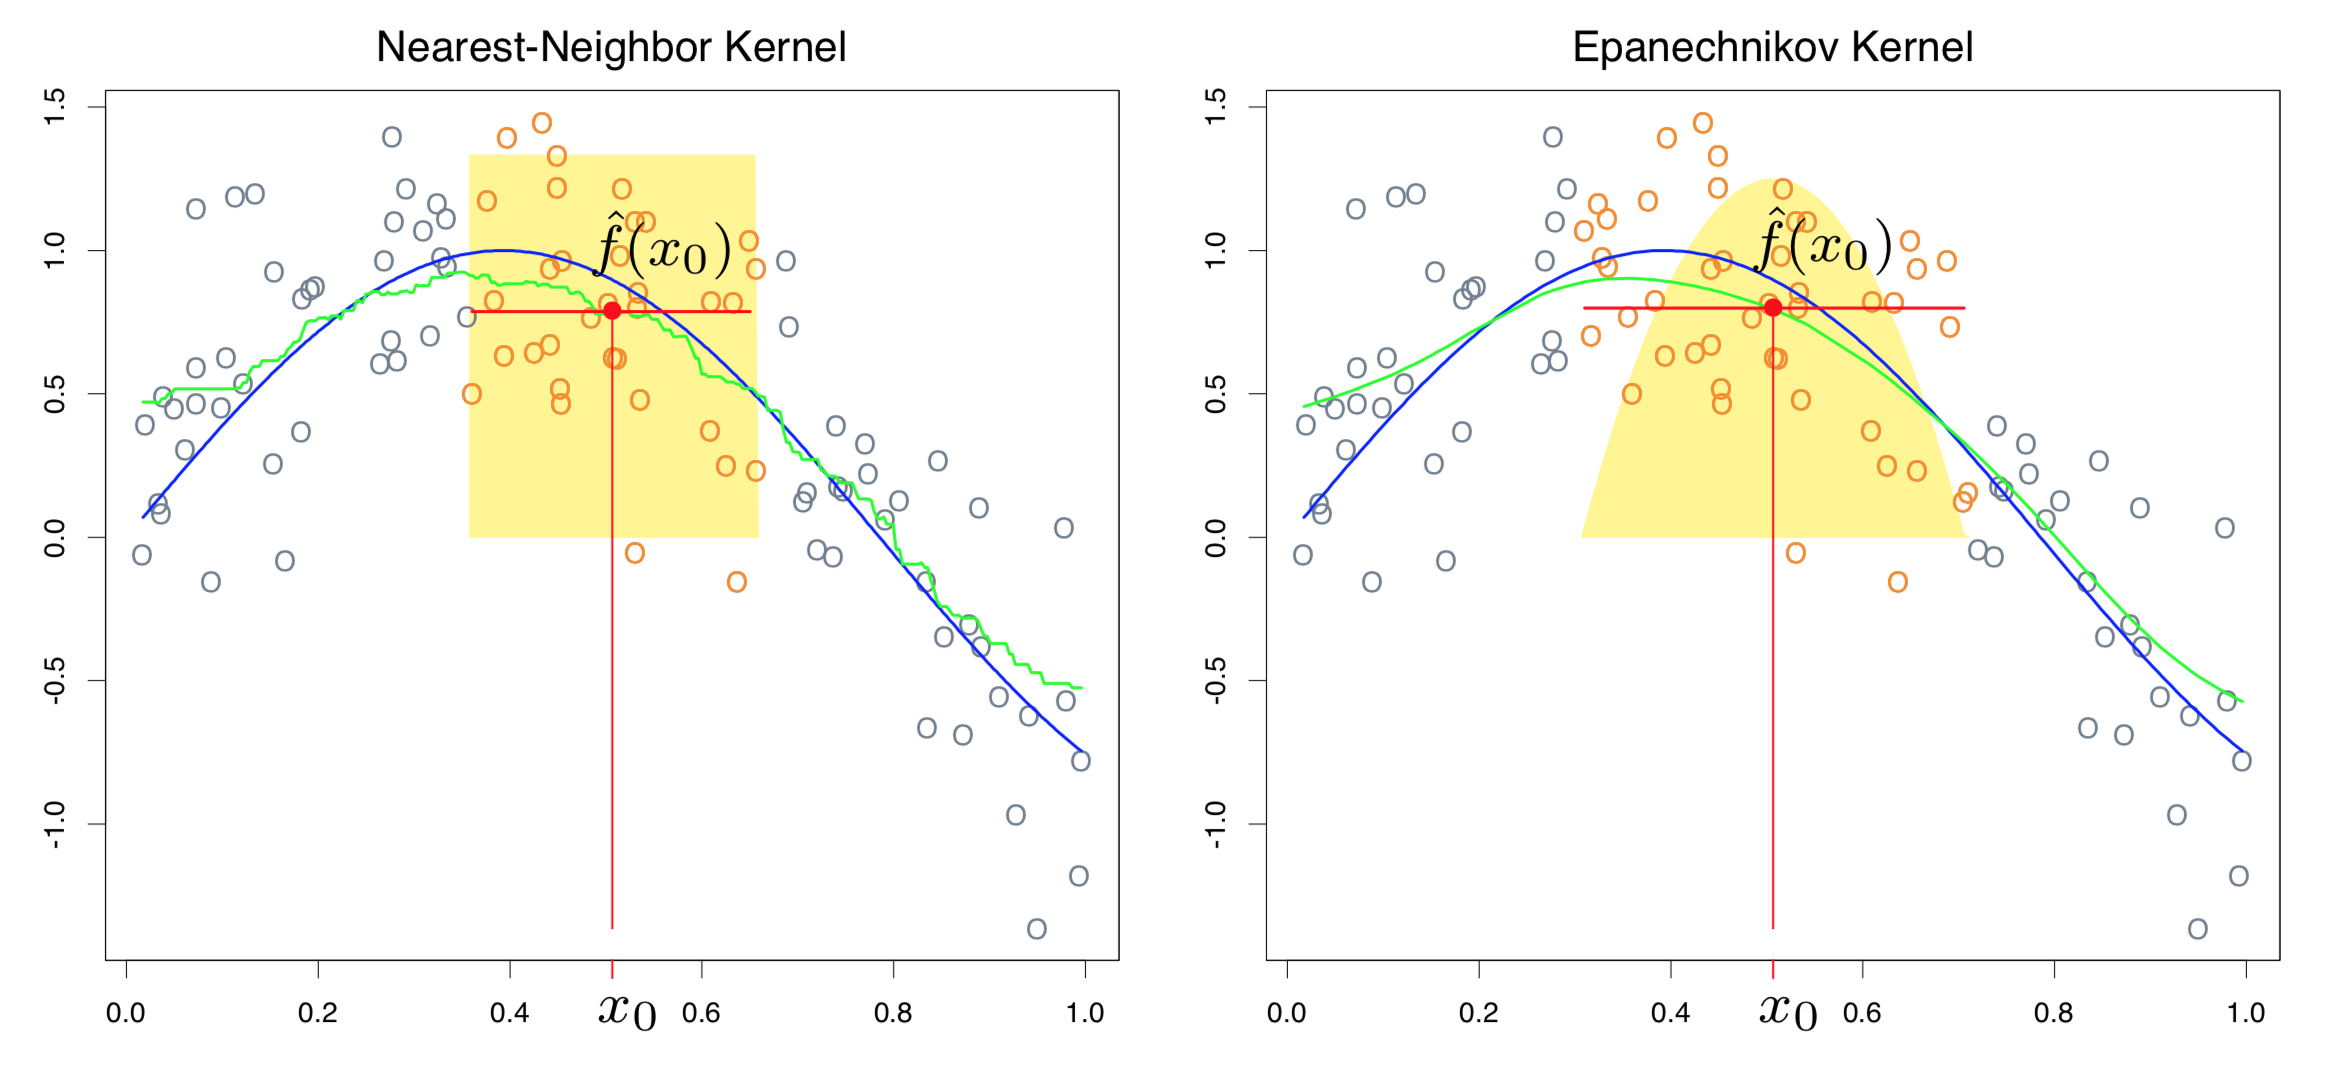
\includegraphics[scale=0.38]{img/nearest}
\caption{In green the fitting curves. On the left the one resulting from \textit{k-nearest neighbourhood}, on the right the metric neighbourhood.}
\label{nearest}
\end{figure}

Rather than give all the points in the neighbourhood equal weights, we can assign weights that die off smoothly with distance from the target point. The right panel in \ref{nearest} shows an example of this, using the so-called Nadaraya–Watson kernel-weighted average:
\begin{equation}
\hat{f}(x) = \frac{K_\lambda(x_0, x_i)y_i}{\sum_{i=1}^N K_\lambda(x_0, x_i)}
\end{equation}
with the Epanechnikov quadratic kernel:
\begin{equation}
K_\lambda(x_0, x_i)= D\br{\frac{|x-x_0|}{\lambda}} = \left\{ \begin{array}{ll}  \frac{3}{4}\left[1-\left(\frac{|x-x_0|}{\lambda} \right)^2 \right]&\quad if \frac{|x-x_0|}{\lambda}\le 1\\
0 &\quad otherwise
\end{array}
 \right.
\end{equation}
Now the function is continuous. As we move the target from left to right, points enter the neighborhood initially with weight zero, and then their contribution slowly increases. Note that $\lambda$ dictates the width of the window which is fixed. On the contrary, for the \textit{k-nearest neighbourhood} the window size depends on the density since anyway $k$ points must be considered. \ref{kernels} shows other kernels. Another popular one is the tri-cube function:

\begin{equation}
 D\br{\frac{|x-x_0|}{\lambda}} = \left\{ \begin{array}{ll}  \left[1-\left(\frac{|x-x_0|}{\lambda} \right)^3 \right]^3&\quad if \frac{|x-x_0|}{\lambda}\le 1\\
0 &\quad otherwise
\end{array}
 \right.
\end{equation}

Both are compact functions. A common non-compact function is the Gaussian function.

Generalizing we can use a width function $h_\lambda(x_0)$ that determines the width of the neighbourhood at $x_0$ (previously we have used $h_\lambda(x_0) = \lambda$.

\begin{figure}
\centering
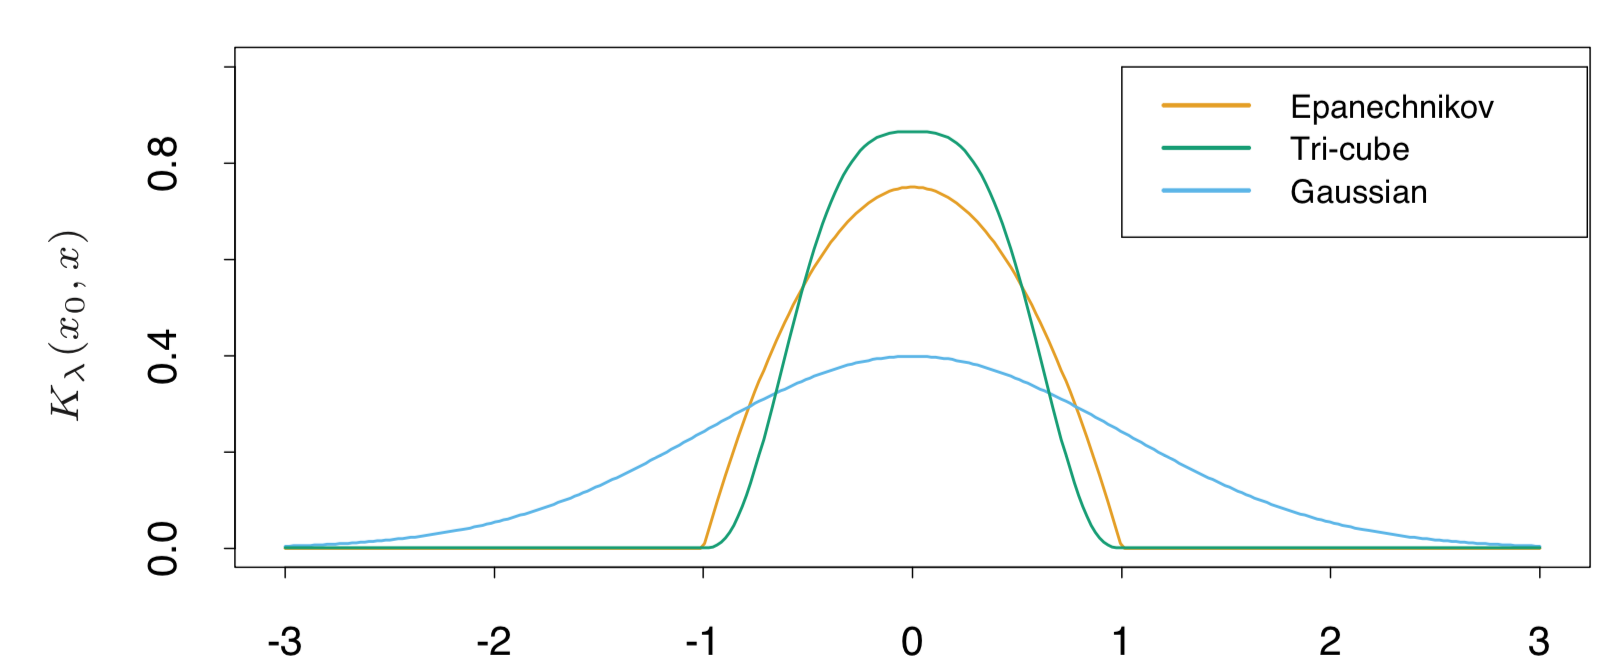
\includegraphics[scale=0.4]{img/kernels}
\caption{A comparison of three popular kernels for local smoothing. Each has been calibrated to integrate to 1. The tri-cube kernel is compact and has two continuous derivatives at the boundary of its support, while the Epanechnikov ker- nel has none. The Gaussian kernel is continuously differentiable, but has infinite support.}
\label{kernels}
\end{figure}

There are a number of details to be clarified:
\begin{itemize}
\item the value of $\lambda$ which selects the window size. Large values imply lower variance but higher bias;
\item $h_\lambda(x_0)$ can be constant (i.e., $h_\lambda(x_0)=\lambda$) or variable. Constant values (\textbf{metric window widths} keep the bias constant but the variance is inversely proportional to the local density. Nearest neighbourhood has opposite behaviour: the variance stays constant and the absolute bias varies inversely with local density.
\item boundary issues: the metric neighbourhood tend to contain less points on the boundaries while the nearest-neighbourhood get wider.
\end{itemize}

\subsubsection{Local linear regression}
Smooth kernel fit still has a problem close to the boundaries: because of the asymmetry in this region weighted averages can be badly biased (left in \ref{biasedKernel}). By fitting straight lines rather than constants locally, we can remove this bias effect. Actually, this bias can be present in the interior of the domain as well, if the $X$ values are not equally spaced.
\begin{figure}
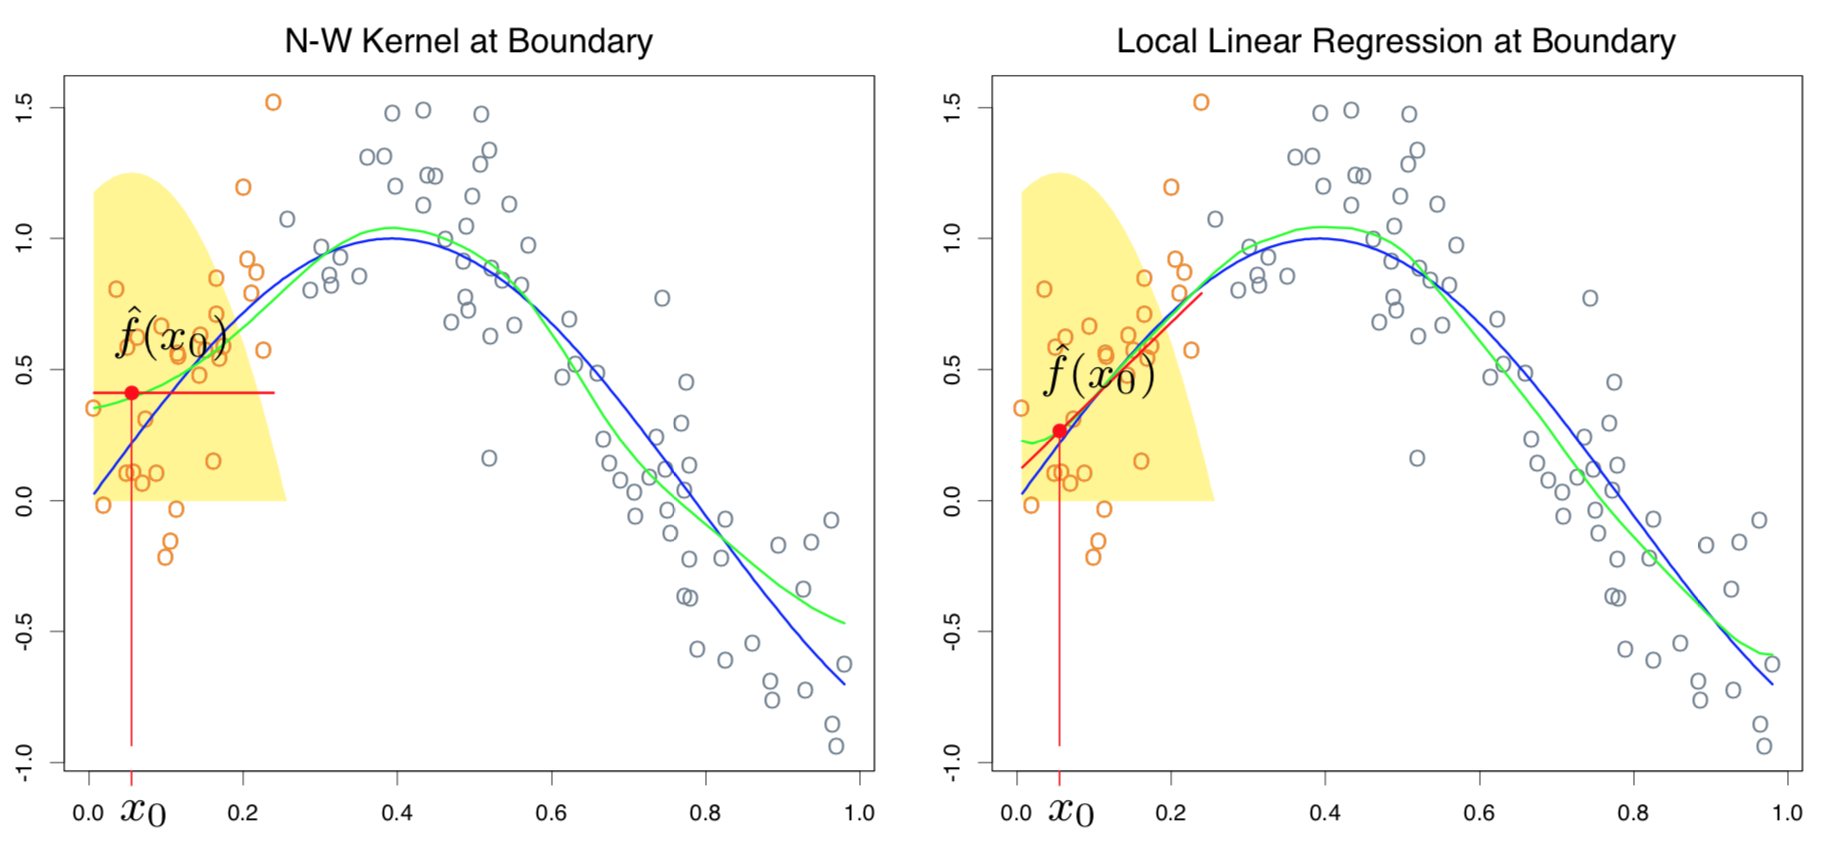
\includegraphics[scale=0.4]{img/biasedKernel}
\caption{On the left it can be noticed the bias effect at the boundaries.}
\label{biasedKernel}
\end{figure}
Locally weighted regression solves a separate weighted least squares problem at each target point $x_0$:
\begin{equation}
min_{\alpha(x_0), \beta(x_0)} \sum_{i=1}^N K_\lambda(x_0,x_1)\left[ y_i - \alpha(x_0) -\beta(x_0)x_i\right]^2
\end{equation}
and the estimate becomes:
\begin{equation}
\hat{f}(x_0) = \hat{\alpha}(x_0) + \hat{\beta}(x_0) x_0
\end{equation}
Notice that although we fit an entire linear model to the data in the region, we only use it to evaluate the fit at the single point $x_0$.

Define the vector-valued function $b(x)^T = (1, x)$. Let $B$ be the $N \times 2$ regression matrix with i-th row $b(x_i)^T$ , and $W(x_0)$ the $N \times N$ diagonal matrix with $i-th$ diagonal element $K_\lambda(x_0,x_i)$. Then
\begin{equation}
\hat{f}(x_0)= b(x_0)^T(\mathbf{B}^T\mathbf{W}(x_0)\mathbf{B})^{-1} \mathbf{B}^T\mathbf{W}(x_0)\y= \sum_{i=1}^N l_i(x_0)y_i
\end{equation}
The weights $l_i(x_0)$ combine the weighting kernel $K_\lambda(x_0, \cdot)$ and the least squares operations and are referred to as the equivalent kernel.Local linear regression automatically modifies the kernel to correct the bias exactly to
first order, a phenomenon dubbed as \textbf{automatic kernel carpentry}.

\subsubsection{Local polynomial regression}
We can fit local polynomial fits of any degree $d$:
\begin{equation}
\begin{aligned}
&min_{\alpha(x_0),\beta_j(x_0),j=1,\cdots,d} \sum_{i=1}^N K_\lambda(x_0,x_i)\left[ y_i - \alpha_0 -\sum_{j=1}^d\beta_j(x_0)x_i^j\right]^2\\
&\hat{f} = \hat{\alpha}(x_0) + \sum_{j=1}^d \hat{\beta}_j(x_0)x_0^j
\end{aligned}
\end{equation}
Local linear fits tend to be biased in regions of curvature of the true function, a phenomenon referred to as \textbf{trimming the hills} and \textbf{filling the valleys}. Local quadratic regression is generally able to correct this bias. There is of course a price to be paid for this bias reduction, and that is increased variance. The fit in the right panel of \ref{localLinQuad} is slightly more
wiggly, especially in the tails.
\begin{figure}
\centering
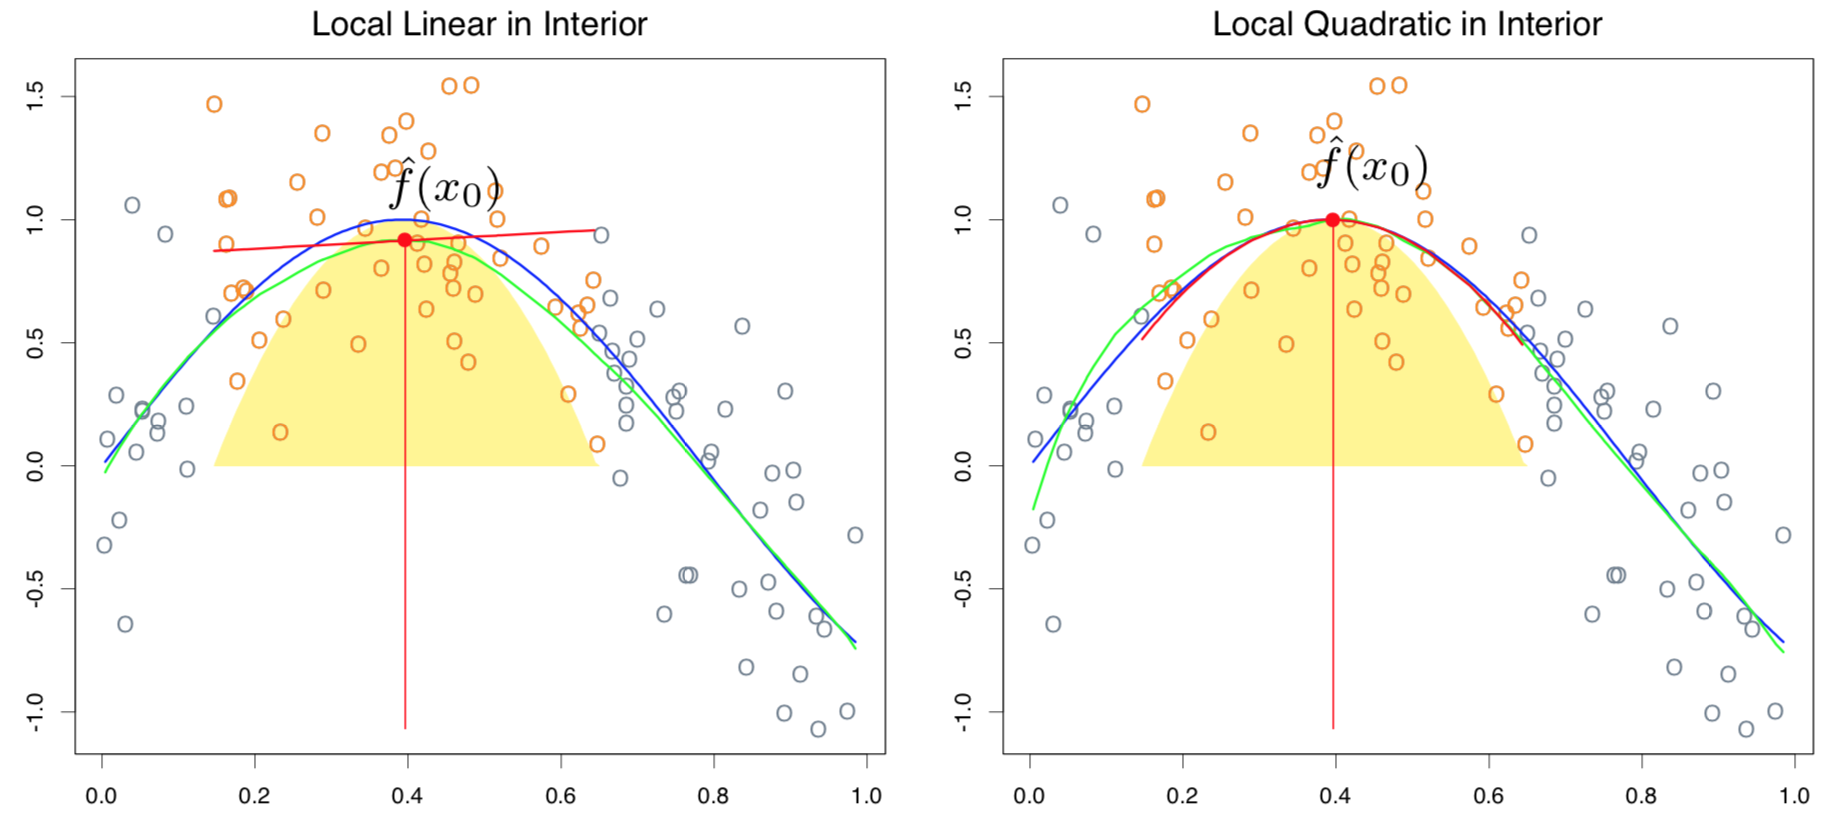
\includegraphics[scale=0.4]{img/localLinQuad}
\caption{Local linear fits exhibit bias in regions of curvature of the true function. Local quadratic fits tend to eliminate this bias.}
\label{localLinQuad}
\end{figure}
Summarizing, local linear fits can help bias dramatically at the boundaries at a modest cost in variance. Local quadratic fits do little at the boundaries for bias, but increase the variance a lot. Local quadratic fits tend to be most helpful in reducing bias due to curvature in the interior of the domain. Asymptotic analysis suggest that local polynomials of odd degree dominate those of even degree. This is largely due to the fact that asymptotically the MSE is dominated by boundary effects.
\subsection{Local regression in $\CMcal{R}^p$}
Let $b(X)$ be a vector of polynomial terms in $X$ of maximum degree $d$. For example, with $d = 1$ and $p = 2$ we get $b(X) = (1,X_1,X_2)$; with $d = 2$ we get $b(X) = (1, X_1, X2, X_1^2, X_2^2, X_1X_2)$; and trivially with $d = 0$ we get $b(X) = 1$. At each $x_0 \in \CMcal{R}^p$ solve:
\begin{equation}
min_{\beta(x_0)} \sum_{i=1}^N K_\lambda (x_0, x_1)\left(y_i - b(x_i)^T\beta\left(x_0\right)\right)^2
\end{equation}
to produce the fit
\begin{equation}
\hat{f} (x_0) = b(x_0)^T\hat{\beta}(x_0)
\end{equation}
While boundary effects are a problem in one-dimensional smoothing, they are a much bigger problem in two or higher dimensions, since the fraction of points on the boundary is larger. In fact, one of the manifestations of the curse of dimensionality is that the fraction of points close to the boundary increases to one as the dimension grows. Directly modifying the kernel to accommodate two-dimensional boundaries becomes very messy, especially for irregular boundaries.  Directly modifying the kernel to accommodate two-dimensional boundaries becomes very messy, especially for irregular boundaries.
Local regression becomes less useful in dimensions much larger than $2$.

For high dimensionality it is impossible to simultaneously maintain localness (i.e., low bias) and a sizable sample in the neighbourhood (low variance) as dimensions increase, without the total sample size increasing exponentially with $p$.

\subsection{Structured local regression models in $\CMcal{R}^p$}
When the dimension to sample-size ratio is unfavorable, local regression does not help us much, unless we are willing to make some structural assumptions about the model.

\subsubsection{Structured kernels}
The default spherical kernel gives equal weight to each coordinate and we can standardize the variables to unit deviation.

Another way is to use a positive definite matrix $A$ to weigh the different coordinates:
\begin{equation}
K_\lambda(x_0, x) = D\left( \frac{(x-x_0)^T\mathbf{A}(x-x_0)}{\lambda}\right)
\end{equation}
Entire coordinates or directions can be downgraded or omitted by imposing appropriate restrictions on $\mathbf{A}$. For example, if $\mathbf{A}$ is diagonal, then we can increase or decrease the influence of individual predictors $X_j$ by increasing or decreasing $A_{jj}$.

\subsubsection{Structured regression function}
We are trying to fit a regression function $\E[Y|X] =f(X_1,X_2, \cdots, X_p)$ in $CMcal{R}^p$ in which every level of interaction is potentially present. It is natural to consider analysis-of-variance (ANOVA) decompositions of the form
\begin{equation}
f(X_1,X_2,\cdots, X_p) = \alpha + \sum_j g_j(X_j) +  \sum_{k<l} g_{kl}(X_k, X_l) + \cdots 
\end{equation}
and then introduce structure by eliminating the higher-order terms. Additive models assume only main effect terms: $f(X) = \alpha + \sum_{j=1}^p g_j(X_j)$, second order models will have terms with interactions of order at most two and so on.  The important detail is that at any stage, one-dimensional local regression is all that is needed. The same ideas can be used to fit low-dimensional ANOVA decompositions.

\subsection{Local likelihood and other models}
Any parametric model can be made local.

For example we can use likelihood local to $x_0$,  with the parameters $\theta(x_0) = x_0^T\beta(x_0)$:
\begin{equation}
l\br{\beta(x_0)} = \sum_{i=1}^N K_\lambda (x_0,x_i) l\br{y_i, x_i^T\beta(x_0)}
\end{equation}

Also time-series can be made local by fitting by local least squares with a kernel in order to vary according to the short-term history of the series.
\subsubsection{Local multiclassifier linear logistic regression}
Consider categorical responses $g_i \in {1,2,\cdots, J}$. The global linear model is:
\begin{equation*}
Pr(G=j|X=x) = \frac{e^{\beta_{j0}+\beta_j^Tx}}{1+\sum_{k=1}^{J-1}e^{\beta_{k0}+\beta_k^Tx}}
\end{equation*}
The local log-likelihood for the class $J$ can be written as:
\begin{equation}
\begin{aligned}
&\sum_{i=1}^N K_\lambda(x_0, x_i) \Bigg\{\beta_{g_i0}(x_0)+ \beta_{g_i}(x_0)^T(x_i-x_0)+\\
& -\log\left[ 1+\sum_{k=1}^{J-1}e^{\beta_{k0}(x_0)+\beta_k(x_0)^T(x_i-x_0)}\right]\Bigg\}
\end{aligned}
\end{equation}
Notice that $\beta_{J0}=\beta_{J}=0$ i.e., the last class is taken as reference. Also, we have centred the local regression at $x_0$, so that the fitted posterior probabilities at $x_0$ are simply:
\begin{equation}
\hat{Pr}\br{G=j, X=x_0} = \frac{e^{\hat{\beta}_{j0}(x_0)}}{1+\sum_{k=1}^{J-1}e^{\hat{\beta}_{k0}(x_0)}}
\end{equation}

\subsection{Kernel density classification}
One can use nonparametric density estimates for classification in a straightforward fashion using Bayes' theorem:
\begin{equation}
\hat{Pr}(G=k|X=x_0) = \frac{\hat{\pi}_k \hat{f}_k(x_0)}{\sum_{j=1}^J\hat{\pi}_k \hat{f}_j(x_0)}
\end{equation}
with $\hat{f}_j$ being a fitted nonparametric density estimates for each class separately.

\subsection{Naive-Bayes classifier}
It assumes that given a class $G=j$, the features $X_k$ are independent:
\begin{equation}
f_j(X) = \prod_{k=1}^p f_{jk}(X_k)
\end{equation}
While this assumption is generally not true, it does simplify the estimation
dramatically since $f_{jk}$ can be estimated separately using one dimensional kernel density estimates.
Despite these rather optimistic assumptions, Naive-Bayes classifiers often outperform far more sophisticated alternatives. The reasons are that although the individual class density estimates may be biased, this bias might not hurt the posterior probabilities as much, especially near the decision regions. In fact, the problem may be able to withstand considerable bias for the savings in variance such a "naive" assumption earns.

\subsection{Radial basis functions}
Radial basis functions combine the idea of basis methods and kernel functions by treating $K_\lambda(\xi, x)$ as a basis function:
\begin{equation}
f(x) = \sum_{j=1}^M K_{\lambda_j}(\xi_j,x)\beta_j = \sum_{j=1}^M D\br{\frac{\|x-\xi_j\|}{\lambda_j}}\beta_j
\end{equation}
A popular choice for $D$ is the standard Gaussian density function. There are several methods to estimate the parameters, among which one of the most common is the least squares. We can optimize the sum-of-squares with respect to all parameters:
\begin{equation}
\min_{\{\lambda_j, \xi_j, \beta_j\}_1^M} \sum_{i=1}^N\br{y_i -\beta_0 -\sum_{j=1}^M \beta_j e^{-\frac{(x_i-\xi_j)^T(x_i-\xi_j)}{\lambda_j^2}}}^2
\end{equation}
This model is referred to as RBF network, with $\xi_J$ and $\lambda_j$ playing the role of weights. This criterion is non-convex with multiple local minima.

Another way is to estimate $\{\lambda_j,\xi_j\}$ separately from $\beta_j$. Often, the kernel parameters $\lambda_j$ and $\xi_j$ are chosen in an unsupervised way using the $X$ distribution alone. One of the method is to fit a Gaussian mixture density model  to the training $x_i$, which provides both the centres $\xi_j$ and the scales $\lambda_j$. Other approaches use cluster methods to locate $\xi_j$ and treat $\lambda_j=\lambda$ as a hyper-parameter.

Using a constant $\lambda$ might create holes-regions (regions that are not fitted by any gaussian) where no kernels has appreciable support. Renormalized radial basis functions solve this problem:
\begin{equation}
h_j(x) = \frac{D\br{\frac{\|x-\xi_j\|}{\lambda}}}{\sum_{k=1}^MD\br{\frac{\|x-\xi_k\|}{\lambda}}}
\end{equation}

\subsection{Mixture Models for Density Estimation and Classification}
The mixture model can be viewed as a kind of kernel method:
\begin{equation}
\begin{aligned}
&f(x) = \sum_{m=1}^M \alpha_m \phi(x, \mu_m,\Sigma_m)\\
&\sum_m \alpha_m =1
\end{aligned}
\label{mix}
\end{equation}
It is possible to use any density instead of the Gaussian densities.

The parameters are usually fit by maximum likelihood, using the EM algorithm. If the covariance matrix is force to be scalar $\Sigma_m = \sigma_m \I$, then \ref{mix} has the form of a radial basis expansion. If $\sigma_m = \sigma >0$ and $M \uparrow $

\section{Model assessment and selection}
\textit{Take a look also at this: https://machinelearningmastery.com/probabilistic-model-selection-measures/}
\begin{definition}{\textbf{Training error}}: it is the average loss over the training samples:
\begin{equation}
\bar{err} = \frac{1}{N}\sum_{i=1}^N L(y_i, \hat{f}(x_i))
\end{equation}

For categorical variables it is:
\begin{equation}
\bar{err}  = -\frac{2}{N} \sum_{i=1}^N \log\hat{p}_k(x_i)
\end{equation}
The "$-2$" in the definition makes the log-likelihood loss for the Gaussian distribution match squared-error loss.
\label{trainErr}
\end{definition}

\begin{definition}{\textbf{Test error:}} with  the term \textit{test error} or \textit{generalization error} we indicate the prediction error over an independent test sample different from the one used for the training and it is indicated as 
\begin{equation}
Err_\tau \left[L(Y,\hat{f}(X)|\tau\right]
\end{equation}
where $\tau$ indicates the training set and $X$ and $Y$ are drawn randomly from their joint distribution.
\end{definition}

\begin{definition}{\textbf{Expected prediction error}}: or \textbf{expected test error} is the expectation of the test.
\begin{equation}
Err = \E\left[ L(Y,\hat{f}(X))\right] =  \E\left[Err_\tau\right]
\end{equation}
\end{definition}

\ref{testErr} shows the prediction errors of the same type of model trained with different training sets in light red and their expectation (average) in dark red.

\begin{figure}
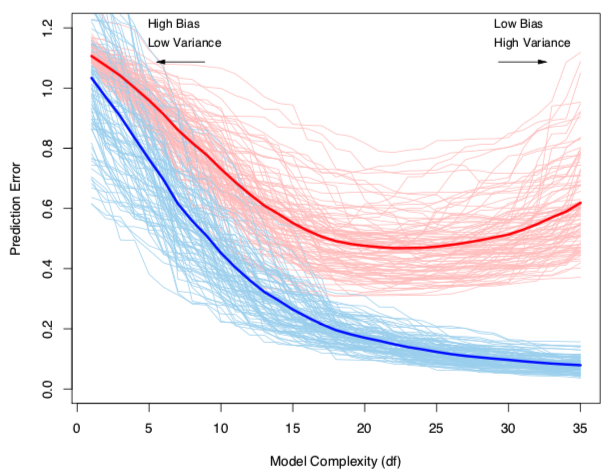
\includegraphics[scale=0.6]{img/testErr}
\caption{Behaviour of test sample and training sample error as the model complexity is varied. The light blue curves show the training error $\bar{err}$, while the light red curves show the conditional test error $Err_\tau$ for $100$ training sets of size $50$ each, as the model complexity is increased. The solid curves show the expected test error $Err$ and the expected training error $E[\bar{err}]$.}
\label{testErr}
\end{figure}
To judge the prediction capability of a model we need to estimate $Err_\tau$. As the model becomes more and more complex, it uses the training data more and is able to adapt to more complicated underlying structures. Hence there is a decrease in bias but an increase in variance. There is some intermediate model complexity that gives minimum expected test error. The training error is not reliable because it always decreases with the model complexity and with too much complexity it looses the capability to generalize.

The same holds for categorical variables (introduced in \ref{trainErr}). Typical loss functions are:
\begin{equation}
\begin{aligned}
&L(G, \hat{G}) = I(G\ne\hat{G}(X)) \quad\quad \textit{0-1 loss},\\
&L(G, \hat{p}(X)) = -2\sum_{k=1}^K I(G=k)\log\hat{p}_k(X) \quad\quad \textit{-2 $\times$ log-likelihood},\\
\end{aligned}
\end{equation}
where the quantity $-2 \times \log-likelihood$ is generally referred as deviance. The "$-2$", as already said, in the definition makes the log-likelihood loss for the Gaussian distribution match squared-error loss.
A number of methods for estimating the expected test error for a model exists. Typically our model will have a tuning parameter or parameters $\alpha$ and so we can write our predictions as$ \hat{f}(x)_\alpha$
The tuning parameter varies the complexity of our model, and we wish to find the value of $\alpha$ that minimizes error, that is, produces the minimum of the average test error curve. There are two goals that one might want to achieve:
\begin{definition}{\textbf{model selection}}: estimating the performance of different models in order to choose the best one.
\end{definition}
\begin{definition}{\textbf{model assessment}}: having chosen a final model, estimate its prediction error on new data.
\end{definition}


If we are in a data-rich situation, the best approach for both problems is to randomly divide the dataset into three parts: a training set, a validation set, and a test set. The training set is used to fit the models; the validation set is used to estimate prediction error for model selection; the test set is used for assessment of the generalization error of the final chosen model. Ideally, the test set should be kept in a "vault", and be brought out only at the end of the data analysis. It is difficult to give a general rule on how to choose the number of observations in each of the three parts, as this depends on the signal-to- noise ratio in the data and the training sample size. A typical split might be 50\% for training, and 25\% each for validation and testing.

The following methods allows to work in a situation with insufficient data. The methods can be distinguished in analytical (AIC, BIC, MDL, SRM) or by efficiently sample re-use (cross-validation and boot-strap). 
Typically the more complex we make the model $f$, the lower the (squared) bias but the higher the variance.
\subsection{Optimism of the training error rate}
Given a training set $\tau$ the generalization error of a model is:
\begin{equation}
Err_\tau = \E_{X^0, Y^0}\left[ L(Y^0, \hat{f}(X^0))|tau\right]
\end{equation}
where the point $(X^0, Y^0)$ is a new test data point. Averaging over training sets $\tau$ (i.e., averaging over the same type of models $\hat{f}$ but trained with different trainsets belonging to the same distribution):
\begin{equation}
Err = \E_\tau \E_{X^0, Y^0}\left[ L(Y^0, \hat{f}(X^0))|tau\right]
\end{equation}
The training error $\bar{err} = \frac{1}{N}\sum_{i=1}^N L(y_i, \hat{f}(x_i))$  will be less than the true error, because the same data is being used to fit the method and assess its error. A fitting method typically adapts to the training data, and hence the apparent or training error $\bar{err}$ will be an overly optimistic estimate of the generalization error $Err_\tau$, which can be thought as \textit{extra-sample error}. 

The nature of the optimism in the training error can be explained considering the \textit{in-sample error}:
\begin{equation}
Err_{in} = \frac{1}{N} \sum_{i=1}^N E_{Y^0}\left[ L(Y_i^0, \hat{f}(x_i))|\tau\right]
\end{equation}
To explain it better consider the same input points $x_i, \quad i=1,\cdots, N$. In the training set for these points we got a given set of values, while on new data we get a slightly different values $Y^0$ due to the random process involved (for example the noise considering the additive model). The model $\hat{f}$ have been trained using the training set, so for its prediction for those points will be close to the values seen in the training set (influenced by randomness) and it cannot foresee the non-deterministic part in the new samples. We define the optimism as the difference between the real $Err_{in}$ and the training error:
\begin{equation}
op \equiv Err_in - \bar{err}
\end{equation} 
and this is typically positive since the second term is generally biased downward. Averaging the optimism:
\begin{equation}
\omega = \E_y(op)
\end{equation}
where the notation $\E_y$ has been used instead of $\E_\tau$ because the predictors (the inputs) are fixed, while the outputs vary.

For squared error, 0-1 loss functions and other loss functions one can show:
\begin{equation}
\omega = \frac{2}{N} \sum_{i=1}^N Cov(\hat{y_i}, y_i)
\end{equation}
Thus the amount by which err underestimates the true error depends on how strongly $y_i$ affects its own prediction. The harder we fit the data, the greater the covariance will be, thereby increasing the optimism. We have the relationship:
\begin{equation}
\E_y (Err_{in}) = \E_y(\bar{err}) +\frac{2}{N} \sum_{i=1}^N Cov(\hat{y_i}, y_i)
\end{equation}
This expression simplifies if $\hat{y}_i$ is obtained by a linear fit with d inputs or basis functions. For example for the additive model $Y=f(X) + \epsilon$:
\begin{equation}
 \sum_{i=1}^N Cov(\hat{y_i}, y_i) = d\sigma_\epsilon^2
\end{equation}
and so
\begin{equation}
\E_y (Err_{in}) = \E_y(\bar{err}) +\frac{2d}{N} \sigma_\epsilon^2
\label{paramSel}
\end{equation}
We can use these expressions to select the effective number of parameters. The optimism increases with the number $d$ of inputs or basis functions we use, but decreases as the training sample size increases

An obvious way to estimate prediction error is to estimate the optimism and then add it to the training error. The methods such as Cp, AIC, BIC and others work in this way, for a special class of estimates that are linear in their parameters.
In contrast, cross-validation and bootstrap methods are direct estimates of the extra-sample error. These general tools can be used with any loss function, and with nonlinear, adaptive fitting techniques.
In-sample error is not usually of direct interest since future values of the features are not likely to coincide with their training set values. But for comparison between models, in-sample error is convenient and often leads to effective model selection. The reason is that the relative (rather than absolute) size of the error is what matters.

\subsection{$C_p$ metric}
One can estimate the in-sample error as
\begin{equation}
\hat{Err} = \bar{err}+\hat{\omega}
\end{equation}
where $\hat{\omega}$ is an estimate of the average optimism. Using \ref{paramSel}:
\begin{equation}
C_p = \bar{err} +\frac{2d}{N} \hat{\sigma}_\epsilon^2
\end{equation}
where $\hat{\sigma}_\epsilon^2$ is an estimate of the noise variance.

The model with lowest $C_p$ should be selected.

\subsection{Akaike Information Criterion}
Suppose we have models $\CMcal{M}_1, \cdots, \CMcal{M}_k$ where each model is a set of densities:
\begin{equation}
\CMcal{M}_j = \left\lbrace p(y;\theta_j):\theta_j \in \Theta_j\right\rbrace.
\end{equation}
and we have data $Y_1,\cdots, Y_n$ drawn from an unknown density $f$ that we do not know if it is in any of the models. Let $\hat{\theta}_j$ be the Maximum Likelihood estimation from the model $j$. Using this we can estimate $f$ with $\hat{p}_j(y) = p(y, \hat{\theta}_j)$. The quality of $\hat{p}_j(y)$ (i.e., its distance form $f$) can be measured by the \textbf{Kullback-Leibler distance}:
\begin{equation}
\begin{aligned}
K(p, \hat{p}_j) &= \int p(y) \log \frac{p(y)}{\hat{p}_j(y)} dy = \\
&=\int p(y) \log p(y) dy  - \int p(y) \log \hat{p}_j(y) dy 
\end{aligned}
\end{equation}
We want to minimize this distance. The first term is constant while we can act on $ \hat{p}_j(y)$. Since it is a probability (i.e.  $\hat{p}_j(y)$ is at most one, minimizing the distance is equivalent to maximizing the second term:
\begin{equation}
K_j = \int p(y) \log \hat{p}_j(y) dy 
\end{equation}
Intuitively one estimate of $K_j$ might be:
\begin{equation}
\bar{K}_j = \frac{1}{N} \sum_{i=1}^N \log p_j(Y_i,\hat{\theta}_j)  = \frac{\ell_j(\hat{\theta_j})}{N} 
\end{equation}
i.e., assuming a uniform distribution. This estimation is very biased because data are being used twice: once for the MLE and the second one to calculate the integral. So we have $\bar{K}_j \ne K_j$. We want to find such difference.

Let us drop the index $j$ (i.e., we are considering just one model and not a set) and just use $K$ and $\bar{K}$. Let $\theta_0$ be the parameters that minimize $K(f,p(\cdot, \theta))$. So $p(y, \theta_0)$ is the closest density in the model to the true density. Let $\ell(y,\theta)=\log p (y, \theta)$ and let us define the \textbf{score} as:
\begin{equation}
s(y,\theta) = \frac{\partial \log p (y, \theta)}{\partial \theta}
\end{equation}
and let $H(y, \theta)$ be the matrix of second derivatives.
Let
\begin{equation}
Z_N = \sqrt{N}\br{\hat{\theta} - \theta_0}
\end{equation}
and recall (?) that :
\begin{equation}
Z_N \rightarrow \CMcal{N}(0, J^{-1}VJ^{-1})
\end{equation}
where 
\begin{equation}
\begin{aligned}
&J = -\E\left[ H(Y,\theta_0\right]\\
& V = Var(s(Y,\theta_0))
\end{aligned}
\end{equation}
Let 
\begin{equation}
S_N = \frac{1}{N}\sum_{i=1}^N s(Y_i, \theta_0)
\end{equation}
By the \textbf{Central Limit Theorem}, and recalling that $\theta_0$ is the value that minimizes $K$ (if it is a convex function then for this value the score is $0$ i.e., $0$ mean):
\begin{equation}
\sqrt{N}S_N \rightarrow \CMcal{N}(0, V)
\end{equation}
since 
\begin{equation}
\begin{aligned}
\Var\left[ \sqrt{N} S_n\right] &= \E\left[ \br{\sqrt{N} S_n - \cancel{\mu_{S_n}}}^2\right]= \\
&= N \E\left[ \br{\frac{1}{N}\sum_{i=1}^N s(Y_i, \theta_0)}^2\right] = \frac{1}{N} \E\left[ \br{\sum_{i=1}^N s(Y_i, \theta_0)}^2\right] =\\
&= \frac{1}{N}  \br{\sum_{i=1}^N \E\left[s(Y_i, \theta_0)\right]^2} =\frac{1}{N} NV=V
\end{aligned}
\end{equation}
Now $J$ is a scalar, considering the distribution $JZ_N$ where $Z_N \rightarrow\CMcal{N}(0, J^{-1}VJ^{-1})$, the result is still a distribution with $0$. For the variance let us use the property:
\begin{equation}
\begin{aligned}
&\Var\left[ JZ_N\right] = J(J^{-1}VJ^{-1})J^T = V\\
&\Rightarrow JZ_N \sim \CMcal{N}(0,V)
\end{aligned}
\label{varMul}
\end{equation}

By using \textbf{Taylor series expansion}:
\begin{equation}
K \approx \int p(y) \br{\log p(y, \theta_0) + \cancel{\br{\hat{\theta} - \theta_0}^Ts(y,\theta_0)}+\frac{1}{2}\br{\hat{\theta} - \theta_0}^TH(y,\theta_0)\br{\hat{\theta} - \theta_0}} dy
\end{equation}
The second term $\br{\hat{\theta} - \theta_0}^Ts(y,\theta_0)$ is $0$ because the score has $0$ mean. Defining 
\begin{equation}
K_0  = \int  p(y) \log p(y, \theta_0)dy
\end{equation}
we have:
\begin{equation}
\begin{aligned}
K &\approx K_0 + \frac{1}{\sqrt{N}}Z_N^T \int H(y,\theta_0) p(y) dy \frac{1}{\sqrt{N}}Z_N  = \\
& =K_0 + \frac{1}{\sqrt{N}}Z_N^T \int H(y,\theta_0) p(y) dy \frac{1}{\sqrt{N}}Z_N = k_0 -\frac{1}{2N} Z_N^TJZ_N
\end{aligned}
\end{equation}
Now applying the \textbf{Taylor series expansion} to $hat{K}$:
\begin{equation}
\bar{K}  \approx \frac{1}{N} \sum_{i=1}^N \br{\ell(Y_i,\theta_0) + \br{\hat{\theta} - \theta_0}^Ts(Y_i,\theta_0)} + \frac{1}{2}\br{\hat{\theta} - \theta_0}^TH(Y_i,\theta_0)\br{\hat{\theta} - \theta_0}
\end{equation}
Defining 
\begin{equation}
\begin{aligned}
&A_N = \frac{1}{N} \sum_{i=1}^N \ell(Y_i, \theta_0) - K_0 = \frac{1}{N} \sum_{i=1}^N \br{\ell(Y_i, \theta_0) - K_0}\\
&J_N = -\frac{1}{N} \sum_{i=1}^NH(Y_i,\theta_0) - \xrightarrow{P} J
\end{aligned}
\end{equation}
we have
\begin{equation}
\begin{aligned}
\bar{K} &\approx K_0 + A_N + (\hat{\theta} - \theta_0)S_N -\frac{1}{2N} Z_N^TJ_NZ_N \approx\\
&\approx K_0 + A_N + \frac{Z_N^T}{N}\sqrt{N}J^{-1}JS_N -\frac{1}{2N} Z_N^TJZ_N  = \\
&= K_0 + A_N + \frac{Z_N^TJZ_N}{N} -\frac{1}{2N} Z_N^TJZ_N
\end{aligned}
\end{equation}
where $\ref{varMul}$ has been used again ($J^{-1}S_N \rightarrow J^{-1}\CMcal{N}(0,V)= \CMcal{N}(0,J^{-1}VJ^{-1}) = Z_N$).
We need another property. Let $\epsilon$ be a random vector with mean $\mu$ and variance $\Sigma$ and let
\begin{equation}
Q = \epsilon^T A \epsilon
\end{equation} 
with $Q$ called a quadratic form. Then
\begin{equation}
\E\left[ Q\right] = trace(A\Sigma)+\mu^TA\mu
\end{equation}
Now taking the difference:
\begin{equation}
\begin{aligned}
\E\left[hat{K}-K\right] &= \E\left[A_N\right]+\E\left[ \frac{Z_N^TJZ_N}{N}\right] = 0 + \frac{trace(J J^{-1}VJ^{-1})}{N}=\\
& \frac{trace(J^{-1}VJ^{-1}J)}{N}= \frac{trace(J^{-1}V)}{N} 
\end{aligned}
\end{equation}
If the model is correct then $J^{-1}=V$ so that $trace(J^{-1}V)= trace(I)=d$:
\begin{equation}
K \approx\hat{K} =  \bar{K} -\frac{d}{N}
\end{equation}
So the bias is approximately $\frac{d}{N}$.
Considering the model $j$:
\begin{equation}
\begin{aligned}
\hat{K}_j &= \bar{K}_j -\frac{d_j}{N}\\
AIC(j) &= 2N \hat{K}_j = \ell_j(\hat{\theta}_j) -2d_j
\end{aligned}
\end{equation}
Maximizing $\hat{K}_j$ is the same as maximising $AIC(j)$. Constants are not important in the maximization process. With this representation we choose the model with the highest AIC.
Other books use the following representation:
\begin{equation}
\begin{aligned}
AIC(j) =-\frac{2}{N}\ell_j(\hat{\theta}_j) +2\frac{d_j}{N}\\
\end{aligned}
\end{equation}
and with this representation the best model is the one that minimizes the AIC, since the signs have been inverted.

For the Gaussian model, with variance $\sigma^2_\epsilon = \hat{\sigma}^2_\epsilon$, the AIC statistic is equivalent to $C_p$.

For non-linear and other complex models we replace $d$ with a measure of the model complexity. Given a set of models $f_\alpha$, $\bar{err}(\alpha)$ is the training error and $d(\alpha)$ the number of parameters:
\begin{equation}
AIC(\alpha) = \bar{err}(\alpha) + 2\frac{d\alpha}{N}\hat{\sigma}^2_\epsilon.
\end{equation}
\subsection{Effective number of parameters}
A linear fitting method (linear regression, derived basis sets and smoothing methods with quadratic shrinkage such as ridge regression and cubic smoothing splines) have the form:
\begin{equation}
\hat{\y} = \mathbf{S}\y
\end{equation}
where $\mathbf{S}$ is a $N\times N$ matrix. The effective number of parameters is defined as:
\begin{equation}
df(\mathbf{S}) = trace(\mathbf{S}) = M
\end{equation}
since $\mathbf{S}$ is an orthogonal projection matrix onto a basis set spanned by $M$ features. Then instead of $d$ we use $trace(\mathbf{S})$.

For models like NN in which we minimize an error function with weight decay penalty (regularization) $\alpha \sum_m w_m^2$, the effective number of parameters has ethe form:
\begin{equation}
df(\alpha) = \sum_{m=1}^M \frac{\theta_m}{\theta_m+\alpha}
\end{equation}
where $\theta_m$ are the eigenvalues of the Hessian matrix $\partial R(\omega) /\partial \omega\partial \omega^T$.

\subsection{Bayesian Information Criterion}
Known also as \textit{Schwarz Criterion}, it is equivalent to the MDL. We choose $j$ to maximize
\begin{equation}
BIC(j) = \ell_j(\hat{\theta}_j) - \frac{d_j}{2}\log n
\end{equation}
It is similar to the AIC but it has a stronger penalization and tends to choose simpler models.

Using priors $\pi_j(\theta_j)$ on the parameters $\theta_j$ and a probability $p_j$ indicating the probability that  $\CMcal{M}_j$ is the true model, by Bayesian theory, indicating with $\mathbf{Z}$ the training set, we have:
\begin{equation}
P(\CMcal{M}_j|\mathbf{Z}) \propto p(\mathbf{Z}|\CMcal{M}_j) p_j
\end{equation}
Furthermore
\begin{equation}
\begin{aligned}
p(\mathbf{Z}|\CMcal{M}_j) &= \int p(\mathbf{Z}|\CMcal{M}_j,\theta_j)\pi_j(\theta_j) d\theta_j = \\
&=\int L(\theta_j)\pi_j(\theta_j) d\theta_j
\end{aligned}
\end{equation}
So equivalently we choose $j$ to maximize:
\begin{equation}
\log \int L(\theta_j)\pi_j(\theta_j) d\theta_j + \log p_j
\end{equation}
Using Taylor expansion:
\begin{equation}
\begin{aligned}
\log \int L(\theta_j)\pi_j(\theta_j) d\theta_j + \log p_j &\approx \ell_j(\hat{\theta}_j) - \frac{d_j}{2}\log n \\
\Rightarrow BIC(j) &= \ell_j(\hat{\theta}_j) - \frac{d_j}{2}\log n
\end{aligned}
\label{BIC}
\end{equation}
The prior has been ignored because it can be shown that the terms involving the prior are lower orders than the ones appearing in \ref{BIC}. Again in some books the signs are inverted.

\textbf{The difference from AIC and Cross-Validation} is that BIC assumes that one of the models is true and that we are trying to find the model most likely to be true in a Bayesian sense. AIC and Cross-Validation tries to find the model that predicts the best.

Under the Gaussian model, assuming the variance $\sigma_\epsilon^2$ is known, with a squared error loss:
\begin{equation}
\begin{aligned}
\bar{err} &=  \sum_i\br{y_i - \hat{f}(x_i)}^2\\
2 \ell_j(\hat{\theta}_j) &= -N\frac{\bar{err}}{\sigma_\epsilon^2}\\
BIC(j) &= -\frac{N}{2\sigma_\epsilon^2}\bar{err} - \frac{d_j}{2}\log n = \frac{N}{2\sigma_\epsilon^2} \left[ \frac{d_j}{N} \sigma_\epsilon^2 \log N - \bar{err} \right]
\end{aligned}
\end{equation}
Hence BIC is proportional to AIC with the factor 2 replaced by $\log N$.

\subsection{Minimum Description Length}
The minimum description length (MDL) principle is a formalization of Occam's razor in which the best hypothesis (a model and its parameters) for a given set of data is the one that leads to the best compression of the data.
The Minimum Description Length is the minimum number of bits, or the minimum of the sum of the number of bits required to represent the data and the model.
$\cdots$

\subsection{Cross-Validation}
It is the simplest and most widely used widely used method for estimating prediction error is cross-validation. This method directly estimates the expected extra-sample error. It consists of dividing data set  in parts: a training set and using an independent test sample from the joint distribution. So one set is used for training and the other to avoid overfitting (to validate the model).

\subsubsection{K-fold cross-validation}
K-fold cross-validation uses part of the available data to fit the model, and a different part to test it.
For the $k-th$ part, we fit the model using the other $K-1$ parts for training and we calculate the prediction error of the fitted model on the $k-th$ part. We do this for all $k=1,\cdots, K$, fitting the model resulting from the previous step using the new partition of data.
Typical choices of $K$ are $5$ or $10$. $K=N$ case is known as live-one-out cross-validation. The higher value of $K$ leads to less biased model (but large variance might lead to overfit), where as the lower value of $K$ is similar to the train-test split approach we saw before.

\subsection{Bootstrap Methods}
The general idea  is to randomly draw datasets with replacement from training data. Samples are constructed by drawing observations from a large data sample one at a time and returning them to the data sample after they have been chosen. This allows a given observation to be included in a given small sample more than once. This approach to sampling is called sampling with replacement. This is done $B$ times, producing $B$ datasets.

For the process we need to decide the number of bootstrap samples and a sample size. Then for each boostrap sample, we refit the model to each of the bootstrap datasets and examine the behaviour of the fits over the $B$ replications.

[From wiki:]
As an example, assume we are interested in the average (or mean) height of people worldwide. We cannot measure all the people in the global population, so instead we sample only a tiny part of it, and measure that. Assume the sample is of size N; that is, we measure the heights of N individuals. From that single sample, only one estimate of the mean can be obtained. In order to reason about the population, we need some sense of the variability of the mean that we have computed. The simplest bootstrap method involves taking the original data set of N heights, and, using a computer, sampling from it to form a new sample (called a 'resample' or bootstrap sample) that is also of size N. The bootstrap sample is taken from the original by using sampling with replacement (e.g. we might 'resample' 5 times from [1,2,3,4,5] and get [2,5,4,4,1]), so, assuming N is sufficiently large, for all practical purposes there is virtually zero probability that it will be identical to the original "real" sample. This process is repeated a large number of times (typically 1,000 or 10,000 times), and for each of these bootstrap samples we compute its mean (each of these are called bootstrap estimates). We now can create a histogram of bootstrap means. This histogram provides an estimate of the shape of the distribution of the sample mean from which we can answer questions about how much the mean varies across samples.

\section{Additive models}
A linear model has the form $\alpha + f_1(X_1) + f_2(X_2) + f_3(X_3) + \cdots$, where $X$ are the predictors.

\subsection{Tree based methods}
Tree-based methods partition the feature space into a set of rectangles, and then fit a simple model (like a constant) in each one.

We restrict attention to recursive binary partitions. We first split the space into two regions, and model the response by the mean of $Y$ in each region. We choose the variable and split-point to achieve the best fit. Then one or both of these regions are split into two more regions, and this process is continued, until some stopping rule is applied.

For example we first split at $X_1 = t_1$. Then the region $X_1 \le t_1$ is split at $X_2 =t_2$ and the region $X_1 >t_1$ is split at $X_1 =t_3$ and so on. To each sub-region we assign a constan as output:
\begin{equation}
\hat{f}(X) = \sum_{m=1}^M c_m I\{(\x \in \CMcal{R}_m\}
\end{equation}
An advantage of this representation is its interpretability. When more than 2 inputs are involved, it is difficult to represent the partition of the input space. 
\begin{figure}
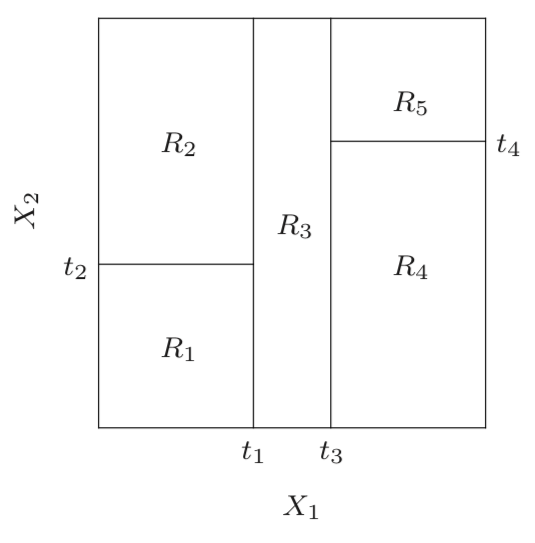
\includegraphics[scale=0.4]{img/tree1}
\caption{2D-input space binary tree partition.}
\label{tree1}
\end{figure}
\begin{figure}
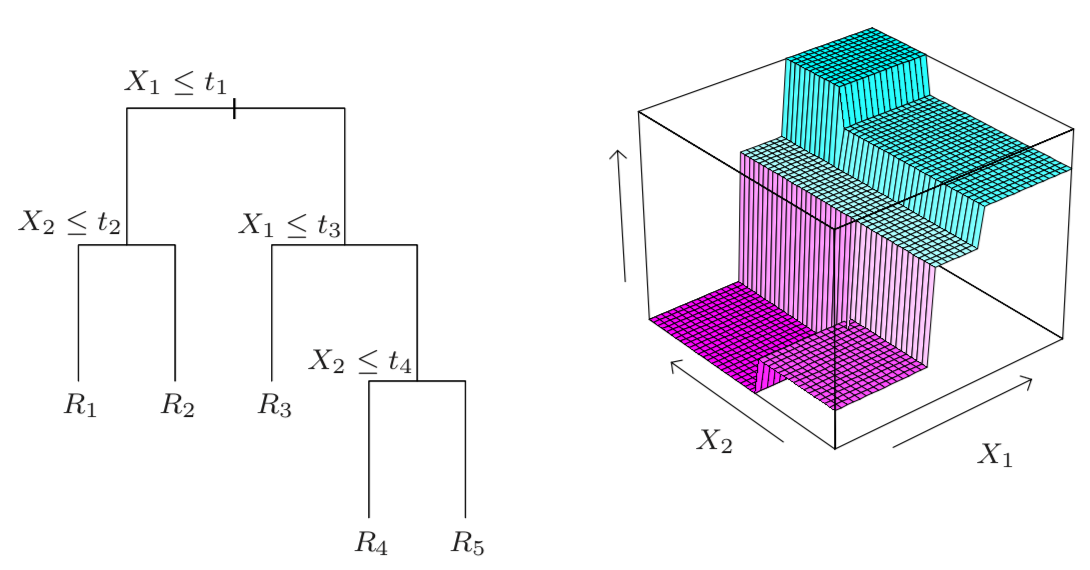
\includegraphics[scale=0.39]{img/tree2}
\caption{Another representation of the binary tree on the left. On the right the 3D resulting shape of the function.}
\label{tree1}
\end{figure}
\subsubsection{Regression Trees}
The algorithm needs to decide automatically the splitting variables and points. We can start defining the values of the constant of each region:
\begin{equation}
\hat{c}_m = ave(y_i|x_i \in CMcal{R}_m)
\end{equation}
Now finding the best binary partition in terms of minimum sum of squares is generally computationally infeasible. Hence we proceed with a greedy algorithm. Consider a splitting variable $j$ and split point $s$ and define the pair of half-planes:
\begin{equation}
R_1(j,s) = \{X|X_j \le s \}. \quad R_2(j,s) = \{X|X_j > s \}
\end{equation}
Then we seek the splitting variable $j$ and split point $s$ that solve:
\begin{equation}
\begin{aligned}
&\min_{j,s}\left[ \min_{c_1} \sum_{x_i \in \CMcal{R}_1(j,s)}  (y_i-c_1)^2 + \min_{c_2} \sum_{x_i \in \CMcal{R}_2(j,s)}  (y_i-c_2)^2\right]\\
&\hat{c}_1 = ave (y_i|x_i \in R_1(j,s)) \\
&\hat{c}_2 = ave (y_i|x_i \in R_2(j,s)) 
\end{aligned}
\end{equation}
For each splitting variable, the determination of the split point s can be done very quickly and hence by scanning through all of the inputs, determination of the best pair $(j, s)$ is feasible. Having found the best split, we partition the data into the two resulting regions and repeat the splitting process on each of the two regions. Then this process is repeated on all of the resulting regions.


Tree size is a tuning parameter governing the model's complexity, and the optimal tree size should be adaptively chosen from the data. One approach would be to split tree nodes only if the decrease in sum-of-squares due to the split exceeds some threshold. This strategy is too short-sighted, however, since a seemingly worthless split might lead to a very good split below it.
The preferred strategy is to grow a large tree $T_0$, stopping the splitting process only when some minimum node size (say 5) is reached. Then this large tree is pruned using \textbf{cost-complexity pruning}.

The \textbf{cost-complexity pruning} is the following. We define a subtree $T$ of $T_0$. obtained by collapsing any number of its internal nodes. We index the terminal nodes by $m$. let $|T|$ denote the number of terminal nodes in $T$ and 
\begin{equation}
\begin{aligned}
&N_m = \#\{x_i \in \CMcal{R}_m\}\\
&\hat{c}_m = \frac{1}{N_m} \sum_{x_i \ in \CMcal{R}_m} y_i\\
Q_m(T) = \frac{1}{N_m} \sum_{x_i \in R_m}(y_i - \hat{c}_m)^2
\end{aligned}
\end{equation} 
We define the cost complexity criterion:
\begin{equation}
C_\alpha (T) = \sum_{m=1}^{|T|} N_m Q_m(T) + \alpha |T|
\end{equation}
The idea is to find for each $\alpha$ the subtree $T_\alpha$ of $T_0$ to minimize such a function.
For each $\alpha$ there is a unique smallest subtree $T_\alpha$ that minimizes $C_\alpha(T)$. To find $T_\alpha$ we use the \textbf{weakest link pruning}: we collapse the internal node that produces the smallest per-node increase and we continue umtil we produce the single-node (root) tree. So we have a sequence of subtrees that must contain $T_\alpha$. We choose $\alpha$ to minimize the cross-validated sum of squares, obtaining the tree $T_\alpha$.

\subsection{Classification trees}
The procedure is very similar. In a node $m$ representing the region $R_m$ with $N_m$ observations, let 
\begin{equation}
\hat{p}_{mk} = \frac{1}{N_m}\sum_{\x_i\in R_m} I(y_i=k)
\end{equation}
We classify the observations in node $m$ to class
\begin{equation}
k(m) =argmax_k \hat{p}_{mk},
\end{equation}
the majority class in node $m$. Different measures $Q_m(T)$ of node impurity exist
\begin{equation}
\begin{aligned}
&\textbf{Misclassification error} \quad \frac{1}{N_m} \sum_{i\in CMcal{R}_m} I(y_i \ne k(m))=1-\hat{p}_{km}\\
&\textbf{Gini index} \quad\quad \sum_{k\ne k'} \hat{p}_{mk}\hat{p}_{mk'} = \sum_{k=1}^K \hat{p}_{mk}(1- \hat{p}_{mk})\\
&\textbf{Cross-entropy or deviance} \quad -\sum_{k=1}^K \hat{p}_{mk}\log \hat{p}_{mk}
\end{aligned}
\end{equation}

These trees are referred as CART (classification and regression trees).
\subsubsection{Linear Combination splits}
Rather than using splits of the type $X_j\le s$ we can use splits of the type $\sum a_j X_j \le s$. The weights $a_j$ and split point $s$ are optimized to minimize the relevant criterion  such as the Gini index.

\subsubsection{Limitations of trees}
One major problem of trees is \textbf{the instability (i.e., high variance)}. A small change in the data can result in a very different series of splits, making interpretation somewhat precarious. The major reason is the hierarchical nature of the process: the effect of an error in the top split is propagated down to all the next splits. The problem can be attenuated but not completely solved.

Another problem of trees is the \textbf{lack of smoothness}. This is not a problem in classification but it is in regression.

Also they are not good at capturing additive structures, such as $Y = c_1 (X_1 < t_1) + c_1 (X_1 < t_1)+\epsilon$ where the noise is $0$ mean. Then a binary tree might make its first split on $X_1$ near $t_1$. At the next level down it would have to split both nodes $X_2$ at $t_2$ in order to capture the additive structure. This is achieved with sufficient data, but it it is a fragile mechanism and can fail in case of many additive effects.
\subsection{Patient rule induction method (PRIM)}
Also PRIM finds boxes in the feature space, but it seeks boxes in which the response average is high. Hence it looks for maxima in the target function, an exercise known as bump hunting. The main box construction method in PRIM works starting with a box containing all of the data. The box is compressed along one face by a small amount, and peeling off a constant portion of data denoted by $\alpha$. Typically $\alpha$ is $0.05$ and $0.1$ of the remaining points at each stage. The face chosen for compression is the one resulting in the largest box mean, after the compression is performed. Then the process is repeated, stopping when the current box contains some minimum number of data points.

After the top-down sequence is computed, PRIM reverses the process, expanding along any edge, if such an expansion increases the box mean. This is called pasting. The result of these steps is a sequence of boxes, with different numbers of observation in each box. Cross-validation, combined with the judgement of the data analyst, is used to choose the optimal box size. Denote by $B_1$ the points in this first box. These points are now removed from the training set and we repeat the two processes (top-down peeling and bottom-up pasting) several times, obtaining for each iteration a new box $B_i$. Each box is defined by a set of rules involving a subset of predictors such as:
\begin{equation}
(a_1 \le X_1 \le b_1) \quad\quad (b_1 \le X_3 \le b_2)
\end{equation}
PRIM can handle a categorical predictor by considering all partitions of the predictor, as in CART. Missing values are also handled in a manner similar to CART. PRIM is designed for regression

\begin{algorithm}[!ht]
Start with all of the training data, and a maximal box containing all of the data;\\

Consider shrinking the box by compressing one face, so as to peel off the proportion $\alpha$ of observations having either the highest values of a predictor $X_j$ or the lowest. Choose the peeling that produces the highest response mean in the remaining box;\\

Repeat step 2 until some minimal number of observations (say 10) remain in the box;\\

Expand the box along any face, as long as the resulting box mean increases;\\

Steps 1-4 give a sequence of boxes, with different numbers of observations in each box. Use cross-validation to choose a member of the sequence. Call the box $B_1$.\\

Remove the data in the box $B_1$ from the dataset and repeat steps 2-5 to obtain a second box. and continue to get as many boxes as desired.
\end{algorithm}

\begin{figure}
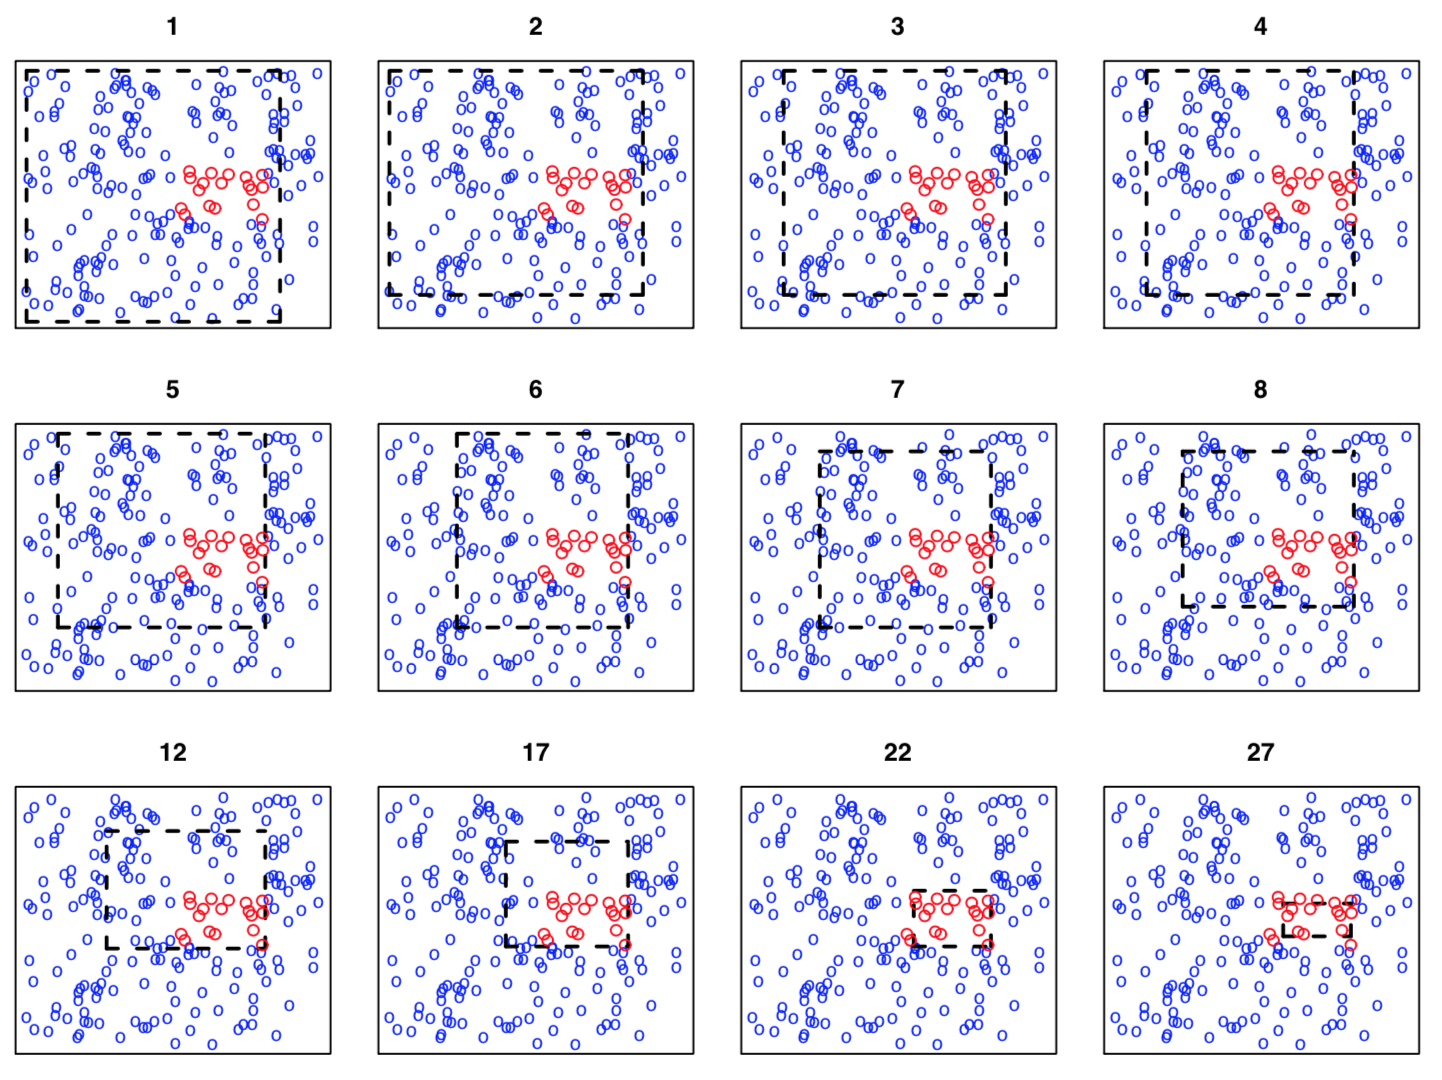
\includegraphics[scale=0.4]{img/PRIM}
\caption{Steps in PRIM.}

\end{figure}
PRIM is designed for binary regression. There is no simple way to deal with $k>2$ classes simultaneously: it is possible to run PRIM separately for each class versus a baseline class.In any case, the ability of PRIM to be more patient should help the top-down greedy algorithm find a better solution.

\subsection{Multivariate Adaptive Regression Splines}
It is a procedure well-suited for high-dimensional problems. MARS uses expansions in piecewise linear basis functions of the form $(x-t)_+$ and $(t-x)_+$.

Each function is piecewise linear, with a knot at the value $t_1$. We call the two functions a \textbf{reflected pair}. The idea is to form reflected pairs for each input $X_j$ with knots at each observed value $x_{ij}$ of that input. If all of the input values are distinct, there are $2Np$ basis functions altogether.
The model-building strategy is like a forward stepwise linear regression, but instead of using the original inputs, we are allowed to use functions from the set $\CMcal{C}$ and their products:
\begin{equation}
\CMcal{C} = \{(X_j-t)_+, (t-X_j)_+\}_{t \in \{x_{1j},\cdots, x_{Nj}\}, j=1,\cdots,p}
\end{equation}
Thus the model has the form:
\begin{equation}
f(X) = \beta_0 + \sum_{m=1}^M \beta_m h_m(X)
\end{equation}
where each $h_m(X)$ is a function in $\CMcal{C}$ or a product of two or more such functions. Given the choice for $h_m(X)$, the coefficients are estimated with the residual sum of squares. We start with only a constant $h_0(X)=1$ and all the functions are candidate functions. At each step we consider as a new basis function pair all products of a function $h_m$ in the model set $\CMcal{M}$ with one of the reflected pairs in $\CMcal{C}$. We add to the model $\CMcal{M}$ the term of the form:
\begin{equation}
\hat{\beta}_{M+1}h_\ell(X) (X_j-t)_+ + \hat{\beta}_{M+2}h_\ell(X) (t-X_j)_+, h_\ell \in \CMcal{M}
\end{equation}
that produces the largest decrease in training error. For example, at the first stage we consider adding to the model a function of the form: $\hat{\beta}_1 (X_2-x_{72})_+ + \hat{\beta}_2(x_{72}-X_2)_+$. Then this pair of basis functions is added to the set $\CMcal{M}$ and at the next stage we consider including a pair of products in the form:
\begin{equation}
h_m(X) (X_j-t)_+ \quad\quad \text{and}\quad\quad h_m(X) (t-X_j)_+, t \in \{x{ij}\}
\end{equation}
where for $h_m$ we have the choices:
\begin{equation}
\begin{aligned}
&h_0(X) = 1\\
&h_1(X) = (X_2 - x_{72})_+,  \quad\textit{or}\\
&h_2(X) = (x_{72} - X_2)_+
\end{aligned}
\end{equation}
At the end of this process we have a large model. This model typically overfits the data, and so a backward deletion procedure is applied. The term whose removal causes the smallest increase in residual squared error is deleted from the model at each stage, producing an estimated best model $\hat{f}_\lambda$ of each size (number of terms) $\lambda$. One could use cross-validation to estimate the optimal value of $\lambda$, but for computational savings the MARS procedure instead uses generalized cross-validation:
\begin{equation}
GCV(\lambda) = \frac{\sum_{i=1}^N (y_i - \hat{f}_\lambda(x_i))^2}{(1-\frac{M(\lambda)}{N})^2}
\end{equation}
The value $M(\lambda)$ is the effective number of parameters in the model: this accounts both for the number of terms in the models, plus the number of parameters used in selecting the optimal positions of the knots.
\end{document} 
